% +--------------------------------------------------------------------+
% | LaTeX Template for K-State Electronic Theses, Dissertations,
% | and Reports
% |
% | Some guidelines for using the template are shown in comments.  Read
% | these comments carefully, as they describe changes you will need to
% | make to the template in order to meet Graduate School requirements.            |
% |
% | Additional information on using the template are contained in these
% | files, which are included when you download the template:
% |
% | ReadMe.pdf - A general overview of using the template
% |
% | BibTeX Guide.pdf - Detailed guidelines on using BibTeX to create
% | your bibliography and manage your citations.
% |
% | natbib.pdf - Gives detailed information on using the natbib package
% | and formatting citations
% +--------------------------------------------------------------------+

% +--------------------------------------------------------------------+
% | The template is designed to be used with PDFLaTeX. Process this
% | file (etdrtemplate.tex) with PDFLaTeX in order to produce a PDF
% | version of your ETDR.  If you are using BibTex to manage your
% | refrences, you will need to process your file four times:
% | 1. Run PDFLaTeX
% | 2. Run BibTex
% | 3. Run PDFLaTeX
% | 4. Run PDFLaTeX
% |
% | Some LaTeX editors do not explicitly list PDFLaTeX as an option, but
% | do use PDFLaTeX to produce a PDF file directly from your .tex files.
% | See the ReadMe file for details.
% +--------------------------------------------------------------------+
% |
% +--------------------------------------------------------------------+
% |
% | As required by the Graduate School, The template is configured to
% | contain the following sections in the order shown.

% | Abstract title page (doctoral dissertations only)
% | Abstract (doctoral dissertations only)
% | Title page
% | Copyright page
% | Abstract
% | Table of contents
% | List of figures
% | List of tables
% | Acknowledgements (Optional)
% | Dedication (Optional)
% | Preface (Optional)
% | Individual Chapters
% | References or Bibliography
% | Appendices (as needed)
% |
% | Details on removing optional sections are given in the comments below.
% |
% +--------------------------------------------------------------------+

% +--------------------------------------------------------------------+
% | The LaTex command \documentclass selects a particular class to
% | associate with the document.  Within this command, 12pt is
% | specified for the font size.  You can change this to 11 pt, if
% | desired.
% +--------------------------------------------------------------------+

\documentclass[final,letterpaper,12pt,oneside]{tex/styles/class_diss}

% +--------------------------------------------------------------------+
% | Here are added external packages that will be used throughout
% | the document.  You can add other packages as needed.
% +--------------------------------------------------------------------+

\usepackage{graphicx} % Extended graphics package.
\usepackage{booktabs} % nice rules (thick lines) for tables
\usepackage{tabulary}
\usepackage{microtype} % improves typography for PDF
\usepackage{xcolor} % Allows color
\usepackage{amsmath} % American Mathematics Society standards
\usepackage{amsxtra} % Additional math symbols
\usepackage{amssymb} % Additional math symbols
\usepackage{amsthm} % Additional math symbols
\usepackage{latexsym} % Additional math symbols
\usepackage{setspace} % Controls line spacing
\usepackage[margin=1in]{geometry} % Sets page margins to 1 inch on all sides
\usepackage[titles]{tocloft} % Adds leader dots to all entries in the table of contents
\usepackage{bm}
\usepackage{tikz}
\usepackage{verbatim}
\usepackage{braket}
\usepackage{longtable}
\usepackage{float}
\usepackage[caption = false]{subfig}


% +--------------------------------------------------------------------+
% | put your own definitions here
% +--------------------------------------------------------------------+

\newcommand{\SN}{S$_N$}
\renewcommand{\vec}[1]{\bm{#1}} %vector is bold italic
\newcommand{\vd}{\bm{\cdot}} % slightly bold vector dot
\newcommand{\grad}{\vec{\nabla}} % gradient
\newcommand{\ud}{\mathop{}\!\mathrm{d}} % upright derivative symbol
\newcommand{\oper}[1]{\mathcal{#1}}
\providecommand{\e}[1]{\ensuremath{\times 10^{#1}}}
\newcommand{\CHAPTER}[1]{Chapter~\ref{#1}} 
\newcommand{\EQ}[1]{Eq.~(\ref{#1})}               %-- Eq. (refeq)
\newcommand{\EQUATION}[1]{Equation~(\ref{#1})}    %-- Equation (refeq)
\newcommand{\FIG}[1]{Fig.~\ref{#1}}               %-- Fig. refig
\newcommand{\FIGURE}[1]{Figure~\ref{#1}} 
\newcommand{\TAB}[1]{Table~\ref{#1}}              %-- Table tablref
\newcommand{\EQS}[2]{Eqs.~(\ref{#1})--(\ref{#2})}            %-- Eqs. (refeqs)
\newcommand{\EQUATIONS}[2]{Equations~(\ref{#1})--(\ref{#2})}   %-- Eqs. (refeqs)
\newcommand{\EQSTWO}[2]{Eqs.~(\ref{#1})~and~(\ref{#2})}     %-- Eqs. (refeqs)
\newcommand{\EQUATIONSTWO}[2]{Equations~(\ref{#1})~and~(\ref{#2})} 

% +--------------------------------------------------------------------+
% |
% | Citation and Bibliography Style
% |
% | The following commands determine the citation and bibliography style.  The
% | template uses BibTeX for formatting the bibliography.  See "BibTeX Guide.pdf"
% | for details on formatting citations and references.  The template is set
% | to use a generic, superscript style, but it can be easily modified
% | to use author-year styles.

\bibliographystyle{unsrtnat}
% | If you want to use an author-year citation style, change "unsrtnat" to
% | "plainnat" in the line above.  You can also use other styles supported
% | by LaTeX, e.g., acm, ieeetr, siam, etc.  Additional styles
% | are in the \styles folder and can be invoked like this:
% | \bibliographystyle{styles/apsrev}.  If the style you use is based
% | on an author-year citation style, you will need to make changes
% | in the usepackage and \setcitestyle statements below

\usepackage[super,sort&compress]{natbib}
% | If you want to use an author-year citation style, change "super" to
% | "authoryear" in the line above.

\setcitestyle{super}
% | if you want to use an author-year citation style, change "super" to
% | "authoryear" in the line above.

% +---------------------------------------------------------------------+
% | The hyperref package enables cross-references.
% +---------------------------------------------------------------------+

\usepackage[pdftex, plainpages=false, pdfpagelabels]{hyperref}

\hypersetup{
    linktocpage=true,
    colorlinks=true,
    bookmarks=true,
    citecolor=blue,
    urlcolor=blue,
    linkcolor=blue,
    citebordercolor={1 0 0},
    urlbordercolor={1 0 0},
    linkbordercolor={.7 .8 .8},
    breaklinks=true,
    pdfpagelabels=true,
    }

% +--------------------------------------------------------------------+
% | The document begins here.
% +--------------------------------------------------------------------+

\doublespacing
\begin{document}

% +--------------------------------------------------------------------+
% | ******Masters Students -- You Need to Make Some Changes Here******
% |
% | The Abstract Title page and Abstract page following the Abstract
% | Title page are required only for doctoral dissertations.  For
% | masters theses or reports, comment out or delete the lines:
% |
% | % +--------------------------------------------------------------------+
% | Abstract Title Page
% |
% |This page is required only for doctoral dissertations.
% +--------------------------------------------------------------------+

% +--------------------------------------------------------------------+
% | This page should not contain a page number.  We use the
% | \thispagestyle[empty] command below to suppress page numbers
% | and other style elements.
% +--------------------------------------------------------------------+

\thispagestyle{empty}

% +--------------------------------------------------------------------+
% | The Abstract Title page begins here
% +--------------------------------------------------------------------+

\pdfbookmark[0]{Title Page}{PDFTitlePage}
%\setcounter{page}{1}

\begin{center}

   \vspace{1cm}

% +--------------------------------------------------------------------+
% | Enter the title of your ETDR below.  For 2017 and on, use "Sentence case" (not ALL CAPS).
% | For details, see:  k-state.edu/grad/etdr/create/sentencecase.html 
% +--------------------------------------------------------------------+

   \large Enter your title in sentence case\\

   \vspace{0.5cm}

   by\\

   \vspace{0.5cm}

% +--------------------------------------------------------------------+
% | Enter your name below in standard name format (not ALL CAPS).
% +--------------------------------------------------------------------+

   \large Enter Your Name\\

   \vspace{0.5cm}

% +--------------------------------------------------------------------+
% | On the line below, replace "Enter Your Previous Degrees"
% | with your previous degrees in mixed case. Include the abbreviation
% | for the degree, the name of the university, and the year separated
% | by commas. For example:
% |
% |    B.A., University of Illinois, 2000
% |
% | If desired, it is acceptable to include a city or country with
% | the university name. For example:
% |
% |    B.S., Jillian University, China, 2002
% |
% | Each degree should appear on a separate line.  Use the \\
% | command to create a line break.
% +--------------------------------------------------------------------+

   Enter Your Previous Degrees\\

   \vspace{0.55cm}
   \rule{2in}{0.5pt}\\
   \vspace{0.75cm}

   {\large AN ABSTRACT OF A DISSERTATION}\\

   \vspace{0.5cm}
   \begin{singlespace}
   submitted in partial fulfillment of the\\
   requirements for the degree\\
   \end{singlespace}

   \vspace{0.5cm}

% +--------------------------------------------------------------------+
% | On the line below, enter the name of your earned degree in ALL
% | CAPITAL LETTERS.  For example: DOCTOR OF PHILOSOPHY
% +--------------------------------------------------------------------+


   {\large ENTER YOUR DEGREE NAME}\\
   \vspace{0.5cm}

% +--------------------------------------------------------------------+
% | On the two lines below, enter the name of your department and the
% | name of the college in mixed case.  For example:
% |
% |     Biochemistry Department
% |     College of Arts and Sciences
% +--------------------------------------------------------------------+

   \begin{singlespace}
   Enter Your Department Name\\
   Enter Your College Name\\
   \end{singlespace}

   \vspace{0.5cm}

   \begin{singlespace}
   {\Large KANSAS STATE UNIVERSITY}\\
   Manhattan, Kansas\\
   \end{singlespace}

% +--------------------------------------------------------------------+
% | On the line below, replace "Graduation Year" with the four-digit year
% | of your graduation. For example:
% |
% |     2017
% +--------------------------------------------------------------------+

   Graduation Year\\
   \vspace{1cm}

\end{center}
 through \end{abstract}.
% |
% | You will also need to uncomment the two lines following the
% | \begin{abstract} command:
% |    %\setcounter{page}{-1}
% |    %\pdfbookmark[0]{Abstract}{PDFAbstractPage}
% |
% | Don't uncomment the lines above.  Scroll down several lines until
% | you see the section "For masters theses or reports, uncomment
% | the commands..." and uncomment the lines in that section.
% +--------------------- ----------------------------------------------+


% +--------------------------------------------------------------------+
% | Title Page -- Required for both Doctoral and Masters Students
% +--------------------------------------------------------------------+

% +--------------------------------------------------------------------+
% | Title Page
% +--------------------------------------------------------------------+

\newpage

% +--------------------------------------------------------------------+
% | This page should not contain a page number.  We use the
% | \thispagestyle[empty] command below to suppress page numbers
% | and other style elements.
% +--------------------------------------------------------------------+

\thispagestyle{empty}

% +--------------------------------------------------------------------+
% | The Title page begins here.
% +--------------------------------------------------------------------+

\begin{center}

   \vspace{1cm}

% +--------------------------------------------------------------------+
% | Enter the title of your ETDR below. For 2017 and on, use "Sentence case" (not ALL CAPS).
% | For details, see: k-state.edu/grad/etdr/create/sentencecase.html 
% +--------------------------------------------------------------------+

\large Origami, Lounge Chairs and Other Topics in Unfolding\\

\vspace{0.5cm}

by\\

\vspace{0.5cm}

% +--------------------------------------------------------------------+
% | Enter your name below in standard name format (not ALL CAPS).
% +--------------------------------------------------------------------+

\large John Charles Boyington\\

 \vspace{0.3cm}

% +--------------------------------------------------------------------+
% | On the line below, replace "Enter Your Previous Degrees"
% | with your previous degrees in mixed case. Include the abbreviation
% | for the degree, the name of the university, and the year separated
% | by commas. For example:
% |
% |    B.A., University of Illinois, 2000
% |
% | If desired, it is acceptable to include a city or country with
% | the university name. For example:
% |
% |    B.S., Jillian University, China, 2002
% |
% | Each degree should appear on a separate line.  Use the \\
% | command to create a line break.
% +--------------------------------------------------------------------+

   B.S., Kansas State University, 2016\\

   \vspace{0.35cm}
   \rule{2in}{0.5pt}\\
   \vspace{0.65cm}

   {\large A THESIS}\\

   \vspace{0.3cm}
   \begin{singlespace}
   submitted in partial fulfillment of the\\
   requirements for the degree\\
   \end{singlespace}

   \vspace{0.3cm}

% +--------------------------------------------------------------------+
% | On the line below, replace "ENTER YOUR DEGREE NAME" with the name
% | of your earned degree in ALL CAPITAL LETTERS.
% +--------------------------------------------------------------------+

   {\large MASTER OF SCIENCE}\\
   \vspace{0.3cm}

% +--------------------------------------------------------------------+
% | On the two lines below, replace "Enter Your Department Name" and
% | "Enter Your College Name" with the name of your department and the
% | name of the college in mixed case.  For example:
% |
% |     Biochemistry Department
% |     College of Arts and Sciences
% +--------------------------------------------------------------------+

   \begin{singlespace}
   Department of Mechanical and Nuclear Engineering\\
   College of Engineering\\
   \end{singlespace}

   \vspace{0.3cm}

   \begin{singlespace}
   {\large KANSAS STATE UNIVERSITY}\\
   Manhattan, Kansas\\
   \end{singlespace}

% +--------------------------------------------------------------------+
% | On the line below, replace "Graduation Year" with the four-digit
% | year of your graduation.  For example:
% |
% |     2016
% +--------------------------------------------------------------------+

   2019\\
   \vspace{0.3cm}

    \end{center}

    \begin{flushright}
    Approved by:\\
    \vspace{0.3cm}
    \begin{singlespace}
    Major Professor


% +--------------------------------------------------------------------+
% | On the line below, replace "Enter Your Major Professor's Name"
% | with  the name of your major professor in mixed case.  Use the
% | format Firstname Lastname.  For example:
% |
% |     Lori Goetsch
% |
% +--------------------------------------------------------------------+

    Jeremy Roberts\\
    \end{singlespace}
    \end{flushright}

% +--------------------------------------------------------------------+
% | If you have co-major professors, comment out the lines above from
% | \begin{flushright} through \end{flushright} and uncomment the
% | lines below.  Enter your co-major professors' names where indicated.
% +--------------------------------------------------------------------+

%\begin{flushright}
%   Approved by:\\
%  \vspace{ 0.3cm}
%   \begin{singlespace}
%   Co-Major Professor\\
%   Enter Your Co-Major Professor's Name\\
%   \vspace{.25cm}
%   Co-Major Professor\\
%   Enter Your Co-Major Professor's Name\\
%   \end{singlespace}
%\end{flushright}


% +--------------------------------------------------------------------+
% | Copyright Page -- Required for both Doctoral and Masters Students
% +--------------------------------------------------------------------+

% +--------------------------------------------------------------------+
% | Copyright Page
% +--------------------------------------------------------------------+

\newpage

\thispagestyle{empty}

\vspace*{0.9cm}

\begin{center}

{\bf \Huge Copyright}

\vspace{1cm}

% +--------------------------------------------------------------------+
% | The Graduate School is using a new 1-line format for 2017 and on, with 
% | the copyright symbol, author name, graduation year and a period at the end.
% | On the line below, replace "Enter Your Name" with your name.
% | Use the same form of your name as it appears on your title page, and 
% |   use mixed case (no more ALL CAPS).  For example:  Barack Obama
% | Replace "YYYY" with the four-digit year of your graduation.  
% | Be sure to include the period  after the year.  
% | EXAMPLE:  © Will E. Wildcat 2017.
% +--------------------------------------------------------------------+

   \Large\copyright\  John Boyington 2019.\\

   \vspace{0.5cm}


\end{center}



% +--------------------------------------------------------------------+
% |  Abstract -- Required for both Doctoral and Masters Students
% +--------------------------------------------------------------------+

\begin{abstract}

% +--------------------------------------------------------------------+
% | For masters theses or reports, uncomment the commands on the next
% | two lines (\setcounter and \pdfbookmark)
% +--------------------------------------------------------------------+

\setcounter{page}{-1}
\pdfbookmark[0]{Abstract}{PDFAbstractPage}

% +--------------------------------------------------------------------+
% | Abstract Page
% +--------------------------------------------------------------------+

\pagestyle{empty}
%\vspace{1cm}
\setlength{\baselineskip}{0.8cm}

%\indent

% +--------------------------------------------------------------------+
% | Enter the text of your abstract below.  There is no limit on the
% | number of words in your abstract.
% +--------------------------------------------------------------------+

Enter the text of your abstract in the abstract.tex file.  Be sure
to delete the text below before you submit your ETDR.

This template uses a separate file for each section of your ETDR:
title page, abstract, preface, chapters, reference, etc.  This
makes it easier to organize and work with a lengthy document.  The
template is configured with page margins required by the Graduate
School and will automatically create a table of contents, lists of
tables and figures, and PDF bookmarks.

The file etdrtemplate.tex is the "master" file for the ETDR
template.  This is the file you need to process with PDFLaTeX in
order to produce a PDF version of your ETDR.  See the comments in
the etdrtemplate.tex and other files for details on using the
template.  You are not required to use the template, but it can save
time and effort in making sure your ETDR meets the Graduate School
formatting requirements.

Although the template gives you a foundation for creating your
ETDR, you will need a working knowledge of LaTeX in order to
produce a final document.  You should be familiar with LaTeX
commands for formatting text, equations, tables, and other
elements you will need to include in your ETDR.

\vfill
\end{abstract}

% +--------------------------------------------------------------------+
% | The following commands start a new page and set the page numbering
% | to lowercase roman numerals.
% +--------------------------------------------------------------------+

\newpage
\pagenumbering{roman}

% +--------------------------------------------------------------------+
% |
% | *********************** IMPORTANT ******************************
% |
% | In the \setcounter command below, set the number to represent the
% | page number of the table of contents page.  For example, if the
% | table of contents page is the 6th page of your document, enter 6
% | in the brackets.  This number may vary, depending on the length of
% | your abstract.
% |
% | Numbers do not appear on the title and abstract pages, but they
% | are included in the page count.  The table of contents page is the
% | first page on which page numbers are displayed.
% +--------------------------------------------------------------------+

\setcounter{page}{4}

% +--------------------------------------------------------------------+
% | The following command creates a bookmark for the table of contents
% | in the final PDF document.
% +--------------------------------------------------------------------+

\pdfbookmark[0]{\contentsname}{contents}

% +--------------------------------------------------------=-----------+
% | The following command adds dot leaders for all entries in the
% | table of contents.
% +--------------------------------------------------------------------+

\renewcommand{\cftchapleader}{\cftdotfill{\cftdotsep}}

% +--------------------------------------------------------------------+
% | The following commands makes all entries and page numbers in the
% | table of contents appear in normal weight font (not bold).
% +--------------------------------------------------------------------+

\renewcommand{\cftchapfont}{\mdseries}
\renewcommand{\cftchappagefont}{\mdseries}

% +--------------------------------------------------------------------+
% | These commands add the table of contents, list of figures, and
% | list of tables.
% +--------------------------------------------------------------------+

\tableofcontents
\listoffigures
\listoftables

% +--------------------------------------------------------------------+
% | Symbols Page
% +--------------------------------------------------------------------+

%\phantomsection
%\addcontentsline{toc}{chapter}{List of Symbols}
%% +--------------------------------------------------------------------+
% | Title Page
% +--------------------------------------------------------------------+

\newpage

\vspace*{0.9cm}
\begin{center}
{\bf \Huge List of Symbols}
\end{center}

% +--------------------------------------------------------------------+
% | This page should not contain a page number.  We use the
% | \thispagestyle[empty] command below to suppress page numbers
% | and other style elements.
% +--------------------------------------------------------------------+

\thispagestyle{empty}

% +--------------------------------------------------------------------+
% | The Symbols page begins here.
% +--------------------------------------------------------------------+

\begin{center}
\begin{longtable}{lll}

\multicolumn{1}{c}{\textbf{Symbol}} & \multicolumn{1}{c}{\textbf{Description}} & \multicolumn{1}{c}{\textbf{Units}} \\ \hline 
\endfirsthead

\multicolumn{3}{c}%
{{\bfseries -- continued from previous page}} \\
\multicolumn{1}{c}{\textbf{Symbol}} &
\multicolumn{1}{c}{\textbf{Description}} &
\multicolumn{1}{c}{\textbf{Unit}} \\ \hline 
\endhead

\multicolumn{3}{r}{{Continued on next page}} \\
\endfoot

\endlastfoot

$\nabla$ & del operator &  \\

\end{longtable}
\end{center}


% +--------------------------------------------------------------------+
% | Acknowledgements Page
% |
% | If you choose not to have an Acknowledgements page, comment out
% | or delete the following 3 lines.
% +--------------------------------------------------------------------+

\newpage
\phantomsection
\addcontentsline{toc}{chapter}{Acknowledgements}
% +--------------------------------------------------------------------+
% | Acknowledgements Page (Optional)
% +--------------------------------------------------------------------+

\newpage
\vspace*{0.9cm}
\begin{center}
{\bf \Huge Acknowledgments}
\end{center}

\setlength{\baselineskip}{0.8cm}

%\pdfbookmark[0]{Acknowledgements}{PDF_Acknowledgements}

% +--------------------------------------------------------------------+
% | Enter text for your acknowledgements in the space below this box.
% |                                                                    
% +--------------------------------------------------------------------+

Enter the text for your Acknowledgements page in the acknowledge.tex
file. The Acknowledgements page is optional.  If you wish to remove
it, see the comments in the etdrtemplate.tex file.


% +--------------------------------------------------------------------+
% | Dedication Page
% |
% | If you choose not to have a Dedication page, comment out
% | or delete the following 3 lines.
% +--------------------------------------------------------------------+

\newpage
\phantomsection
\addcontentsline{toc}{chapter}{Dedication}
% +--------------------------------------------------------------------+
% | Dedication Page (Optional)
% +--------------------------------------------------------------------+

\newpage
\vspace*{0.9cm}
\begin{center}
{\bf \Huge Dedication}
\end{center}

\setlength{\baselineskip}{0.8cm}

\pdfbookmark[0]{Dedication}{PDF_Dedication}

% +--------------------------------------------------------------------+
% | Enter the text for your dedication in the space below this box.    
% +--------------------------------------------------------------------+

\vspace{0.3\textheight}

\begin{center}
{\it To my family}
\end{center}


% +--------------------------------------------------------------------+
% | Preface Page
% |
% | If you choose not to have a Dedication page, comment out
% | or delete the following 4 lines.
% +--------------------------------------------------------------------+

%\newpage
%\phantomsection
%\addcontentsline{toc}{chapter}{Preface}
%% +--------------------------------------------------------------------+
% | Preface (Optional)
% +--------------------------------------------------------------------+

\newpage
\vspace*{0.9cm}
\begin{center}
{\bf \Huge Preface}
\end{center}

\setlength{\baselineskip}{0.8cm}

%\pdfbookmark[0]{Preface}{PDF_Preface}

% +--------------------------------------------------------------------+
% | Enter text of your Preface in the space below this box.            
% +--------------------------------------------------------------------+

Enter the text for your Preface page in the preface.tex file. The
Preface page is optional.  If you wish to remove it, see the
comments in the etdrtemplate.tex file.



% +--------------------------------------------------------------------+
% | This is where the chapter content of your ETDR begins.
% +--------------------------------------------------------------------+

%\phantomsection
\newpage
\pagenumbering{arabic}
\setcounter{page}{1}

% +--------------------------------------------------------------------+
% | Individual chapters of your ETDR are added using the \input
% | command.
% +--------------------------------------------------------------------+


\cleardoublepage


\chapter{Introduction and Background}

% state the general topic and give some background

% provide a review of the literature related to the topic

% define the terms and scope of the topic

% outline the current situation

% evaluate the current situation (advantages/disadvantages) and identify the gap

% identify the importance of the proposed research

% state the research problem/questions

% state the research aims and/or research objectives

% state the hypothese

% outline the order of information in the thesis

% outline the methodology

\cleardoublepage

\chapter{Review of Available Methods and Data}


%%%%%%%%%%%%%%%%%%%%%%%%%%%%%%%%%%%%%%%%%%%%%%%%%%%%%%%%%%%%%%%%%%%%%%%%%%%%%%%%
\section{Beam Port Characterization Experiments}

(Placeholder text)
When measuring charged particles, the energy is directly measurable, which is nice.
You can't do that with neutrons because they are neutral particles, which is less nice.
Instead, most modern methods use discrete responses of individual detectors or detector configurations.

Will talk about Bonner Spheres and Foil Activation here.

%%%%%%%%%%%%%%%%%%%%%%%%%%%%%%%%%%%%%%%%%%%%%%%%%%%%%%%%%%%%%%%%%%%%%%%%%%%%%%%%
\section{Spectral Unfolding Methods}


% ------------------------------------------------------------------------------
\subsection{Formulation}


In practice, active and passive detectors and measurement techniques can appear very different.
However, for the purpose of mathematical formulation, it is possible, and indeed useful, to abstract their similitudes.
The above mentioned detection methods are resemblant in the fact that they provide a set of unique, discrete responses in the presence of an unknown, continuous neutron flux.
These discrete responses can vary greatly between different neutron environments.
For example, the LiI detection crystal of the BSS responds strongly in the presence of thermal neutrons and shows indifference towards neutrons of the faster variety, whereas certian reactions utilized in activation foil analysis, such as ($n, \alpha$), will not occur below specific, fast, threshold neutron energies and the detector is considered to have a fast response.
These largely energy-dependent responses, often related to material properties and reaction cross sections, can be considered functions.
A detector's `Response Function', now formally stated, is the measureable effect exhibited by a detector in a particular geometric configuration as a function of energy to a particular neutron source.
It is true that the response function is more technically also a function of parameters like geometry, source angle and position, etc.; however, it proves efficacious to hold those details constant and consider response unidimensional in energy.




% ------------------------------------------------------------------------------
\subsection{Proposed Methods}


%                   -------------------------------------

\subsubsection{MAXED}




%                   -------------------------------------

\subsubsection{Gravel}

%                   -------------------------------------

\subsubsection{STAY'SL}




%%%%%%%%%%%%%%%%%%%%%%%%%%%%%%%%%%%%%%%%%%%%%%%%%%%%%%%%%%%%%%%%%%%%%%%%%%%%%%%%
\section{Variance Reduction Methods}



\cleardoublepage


\chapter{Introduction}

% here, introduce the ideas present in chapter 3
This section contains a complete description of the neutronic modeling for the NEBP.
% before you measure it, it helps to have a model
It's often necessary, as in this case, to model a neutronic environment before attempting to measure it, as the modeling results can inform certain measurement methods and parameters.
The measurement systems used in later analyses required calculated response functions which built-in the flux's angular dependence obtained from this modeling effort.
The final result from this section also provides the default spectrum to ultimately be used in the unfolding of the final neutron spectrum after measurement.
% there were many problems encountered along the way that lengthened the process of obtaining the final results, most regarding computation time
Many problems were encountered during this analysis, often related to computational difficulty/time, that lengthened the process of obtaining the final results.
These problems, along with the applied solutions, are presented.
% first mcnp kcode, then sdef, then advantg, then finally the tally results
We begin with the NEBP model's KCODE implementation in MCNP, followed by a conversion to a steady-state problem, the application of variance reduction, and finally, the beam-aperture tally results.
% the steps here ultimately led to success in solving a difficult transport problem and could be used in other things like this.
The steps here ultimately led to success in solving a difficult transport problem and these steps taken can likely be applied to similar situations, such as other reactor beam transport problems or, more broadly speaking, any problem with severe collimation of an isotropics source.


\cleardoublepage


\chapter{Experimental Validation}


\section{Introduction}

% -------------------------------------------------------------------------------------------
\section{Modeling}

\subsection{NEBP Decoupling}

% why model?
Before conducting any flux measurement of the beam port, the experimental setups were first modeled in MCNP.
The purpose of this is twofold: one, this generates predictive detector responses to aid in the selection of experimental parameters and provides a metric for the accuracy of initially measured results, and two, response functions are generated for the devices that are ultimately used in the unfolding of the final spectrum.
% can i use the full model?
However, due to the (computational) size of the full reactor model, it would be very expensive to generate these experimental responses and response functions.
Also, the beam port flux, not in-core source spectrum is what we desire to measure, so the response functions would not relate back to the proper flux using the full model.
% no, we need a decoupled model
Necessarily, a decoupled model of the beam and experimental configurations must be used for this portion of the simulation.
This will simplify the geometry and transport significantly, allowing for reduced computation times and also for the ultimate unfolding of the correct neutron spectrum.
% is it valid to decouple?
As to the validity of this decoupling, as long as the full surface current leaving the outer boundary of the full model is captured in the decoupled model, then this approach is neutronically equivalent to a non-decoupled approach.
% yeah, as long as the coupled surfaces capture the outgoing flux, in our case that's justified because a vast majority comes down the beam
In our case, as indicated by the flux results from the previous chapter, the vast majority of departing neutrons leave the beam through the collimator void.
The tallies include a large area around this beam, too, to account for any neutrons that escape the beam.
This flux value decreases rapidly further from the center of the beam, and so it is believed that any neutrons that escape the collimator, leave through the structural material around the collimator, and still manage to interact in any detector will contribute in a statistically insignificant way.

% what does the decoupled model include?
The decoupled model includes the 8" outer portion of the NEBP, which would account for any backscattering from either detector.
% well, i converted the tally into a source at the surface 
The tally from the full model was converted into a steady-state source placed at the outer face of the NEBP.
% the beam and space outside contain universes that different detectors can be included in
The collimator void and space outside of the NEBP contain universes that allow different detectors to be swapped in and out of the model.
% the whole thing is wrapped and driven by python, too so that's great
The entire decoupled model is wrapped in python to allow for variation in input parameters and for the easy extraction and processing of output data.


\subsection{Gold Foil Tube}

% the foil tube was a type of spectrometer
The gold foil tube is a kind of neutron spectrometer.
% the gold foil tube design was based on the bonner sphere - thermal responsing detector with varying moderation
In design, it is principally based on the bonner sphere spectrometer.
Gold foils, which preferentially absorb thermal neutrons are spaced with sections of high density polyethylene (HDPE).
% produce independent responses
HDPE is a strong neutron moderator, meaning that the response of each foil will be somewhat independent of the others, since neutrons are slowing down and being absorbed between foils.
% it was also meant to help with beam alignment and to simplify the beam characterization process
This design also is advantageous in that it solves issues with beam alignment and only requires a single irradiation to generate multiple responses.

%
%\begin{figure}[htb]
%\centering
%\includegraphics[height=4in]{tex/figures/.png}
%\caption[]{}
%\label{fig:}
%\end{figure}


% you can see the device in FIG
The gold foil device can be seen in FIG.
% there are three major components, the aluminum tube, the hdpe separators and the gold foils
The tube is comprised of three separate materials, the gold foils, the HDPE separators, and the aluminum containment tube.
% the gold foils are __ diameter and __ thickness
Each of the gold foils are 5$mm$ in diameter and 0.1$mm$ thick.
% the hdpe was cylinders of __ size
The HDPE sections were 1" thick cylinders.
% each hdpe piece had a __ size hole drilled into it where the gold foil would be situated
A 1$mm$ depth, 5$mm$ OD hole was drilled into the front of each section where the gold foil was situated.
% all of these would be encased in __ID __OD aluminum tubing
All of these sections were sandwiched together and encased in 0.75" OD, 1/24" thick aluminum tubing.
% aluminum is chosen because it's relative insensitivity towards neutrons
Aluminum was chosen because of its relative insensitivity to neutrons.
% the whole apparatus had __ hdpe pieces and foils, with the first foil being exposed and a gap of __ at the beginning
The whole apparatus was comprised of 12 HDPE pieces and foils, with the first, exposed foil being situated 1" from the start of the tubing.

% this device was modeled in mcnp, where f4 flux tallies, folded with the au n,g response were used with a scx card to produce the rfs
This device was modeled in MCNP, where f4 flux tallies, folded with the $^{198}$Au(n,$\gamma$) cross sections were used with an SCX card to produce the response functions.

\subsection{Bonner Sphere Spectrometer}

% a second, active detector was included in the experiment, too, the bss
A second, active detector was also used in the spectrometric section of the NEBP analysis, too, the Bonner Sphere Spectrometer (BSS).
% the bonner sphere spectrometer uses a series of plastic spheres surrounding a lithium iodide detector to produce independent responses
The bonner sphere, while explained more thoroughly in chapter 2, use a series of plastic sphere surrounding a LiI detector to produce independent neutronic responses.

%
%\begin{figure}[htb]
%\centering
%\includegraphics[height=4in]{tex/figures/.png}
%\caption[]{}
%\label{fig:}
%\end{figure}



% you can see the device in FIG
This device can be seen modeled in FIG.
% the full device was modeled using the 4x4 mm detection crystal coupled with pmt and hdpe sphere
The main feature of the device was the 4x4$mm$ detection crystal located at the center of the sphere, although smaller details were also captured with the model, including the photomultiplier tube and some of the detector casing material.
% positioned a distance of __ from the bp aperture
The device was positioned a distance of (???) from the NEBP aperture.
% rfs were generated for sphere sizes of __ __ __ whatver
Response functions were generated for the bare response, as well as the 2", 3", 5", 8", 10", and 12" spheres.
% the tally used f4 folded with the n,t reaction in the crystal with the scx card again
The F4 flux tally over the detection crystal was folded with the (n,t) reaction cross section and an SCX card was again used to produce response functions.



\subsection{Response Functions}

% describe any post processing used for these results to get the values in cm2

Post processing for the gold foil tube and BSS response functions is relatively straightforward.
The response function value for energy $j$, $R_j$, is multiplied by the number of energy groups, $n_{groups}$ and then converted from $b$ to $cm^2$.
This is because the SCX card, which allows a user to tally based on what source distribution bin a particle was born in, will naturally be weighted by the probability of a particle being born in that bin.
To generate the response functions, all bins were considered equiprobable, which means that the true result requires the simple multiplying by the number of bins.
The $cm^2$ conversion is because flux is generally understood in $cm^{-2}s^{-1}$, so using response functions in these units allows one to avoid that conversion later.

\begin{equation}
\label{eqn:postprocessing_au}
R_j = R_{j, mcnp} \times n_{groups} \times 10^{-24}
\end{equation}


% the gold foil tube response functions
\begin{figure}[htb]
\centering
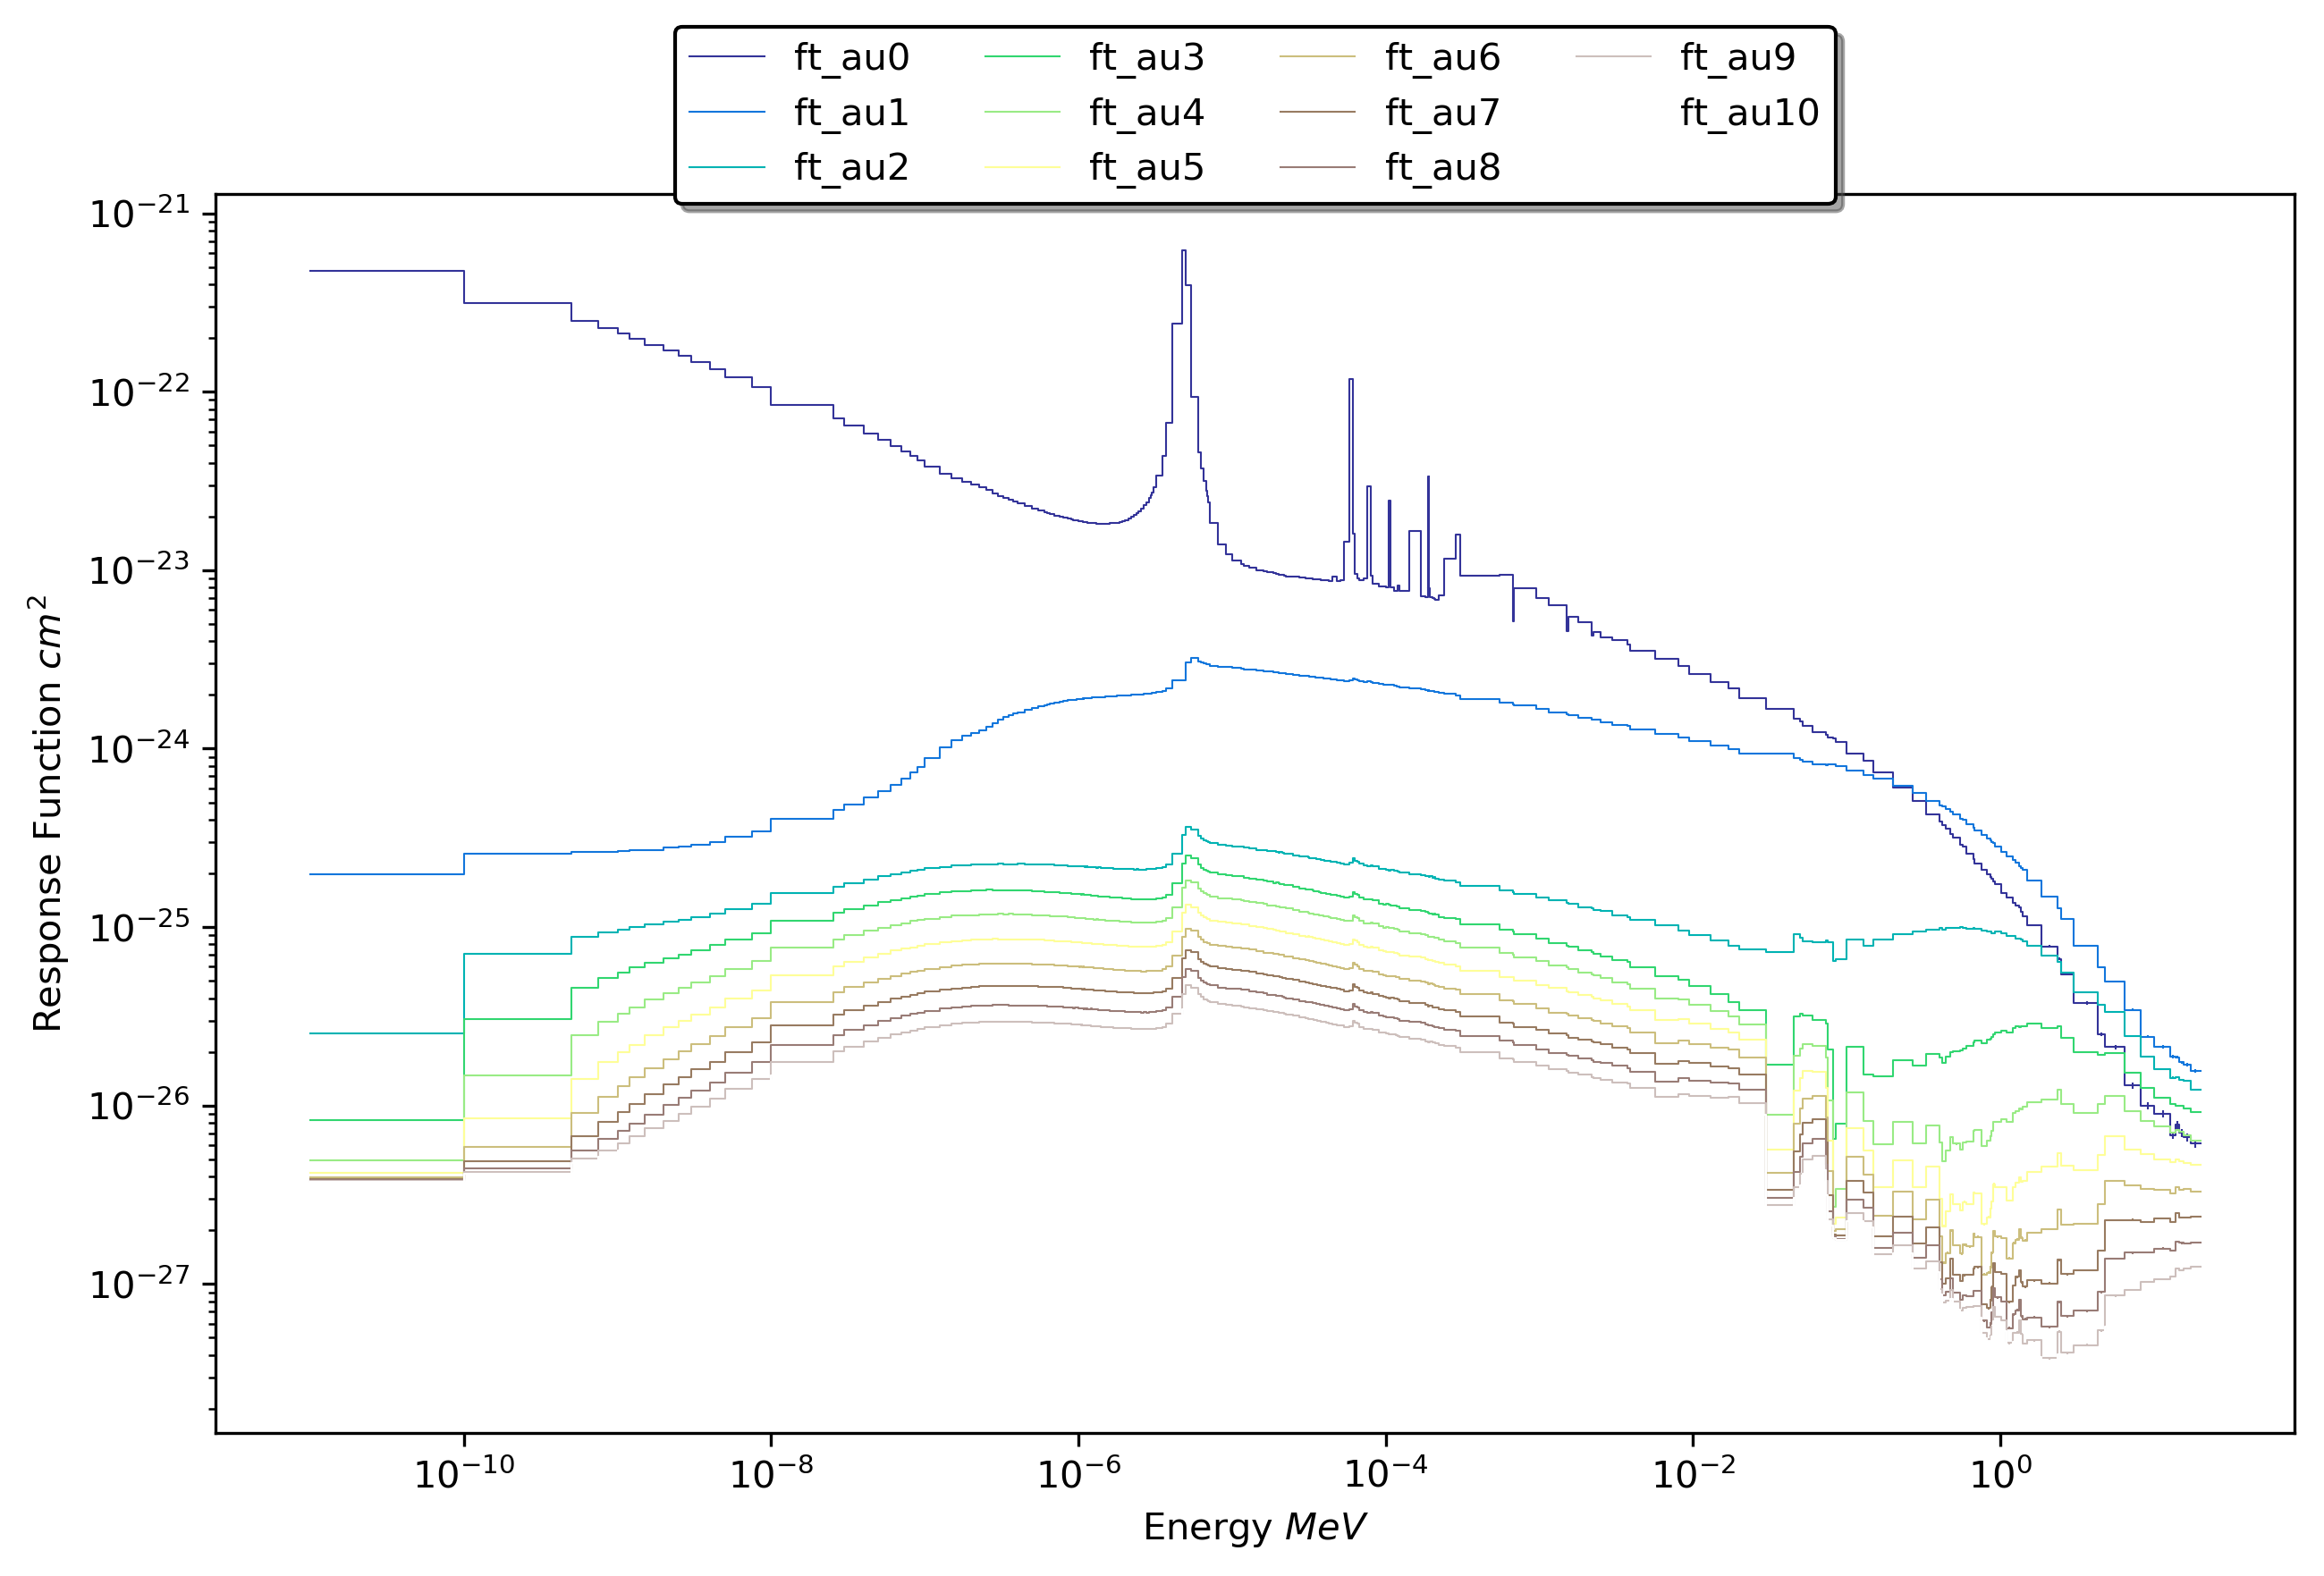
\includegraphics[height=4in]{tex/figures/ft_au.png}
\caption[Gold Foil Tube Response Functions]{The response functions for the gold foil tube.}
\label{fig:ft_au_rfs}
\end{figure}

% discuss the ft_au response functions
The response functions for the gold foil tube are pictured in \FIG{fig:ft_au_rfs}.
As distance from the tube front increases, many interesting features form and decay.
The first response very closely resembles the $^{198}$Au(n,$\gamma$) reaction, since it is exposed to the source and backscattering contributes relatively little to this response.
However, the addition of HDPE tapers the thermal tail of this response very quickly and shifts peak behavior towards the right.
The four sections that follow the first actually have an even higher response than the exposed foil.
Throughout the epithermal region, the relatively slow curvature doesn't seem much affected by the increasing foil distance, but in the fast region, a peak forms after 2", and then grows (relatively) and is pushed to the right as foil distance increases.
Overall, the goal of producing response functions that are independent was met to at least some degree with this device design.

% the bonner sphere response functions
\begin{figure}[htb]
\centering
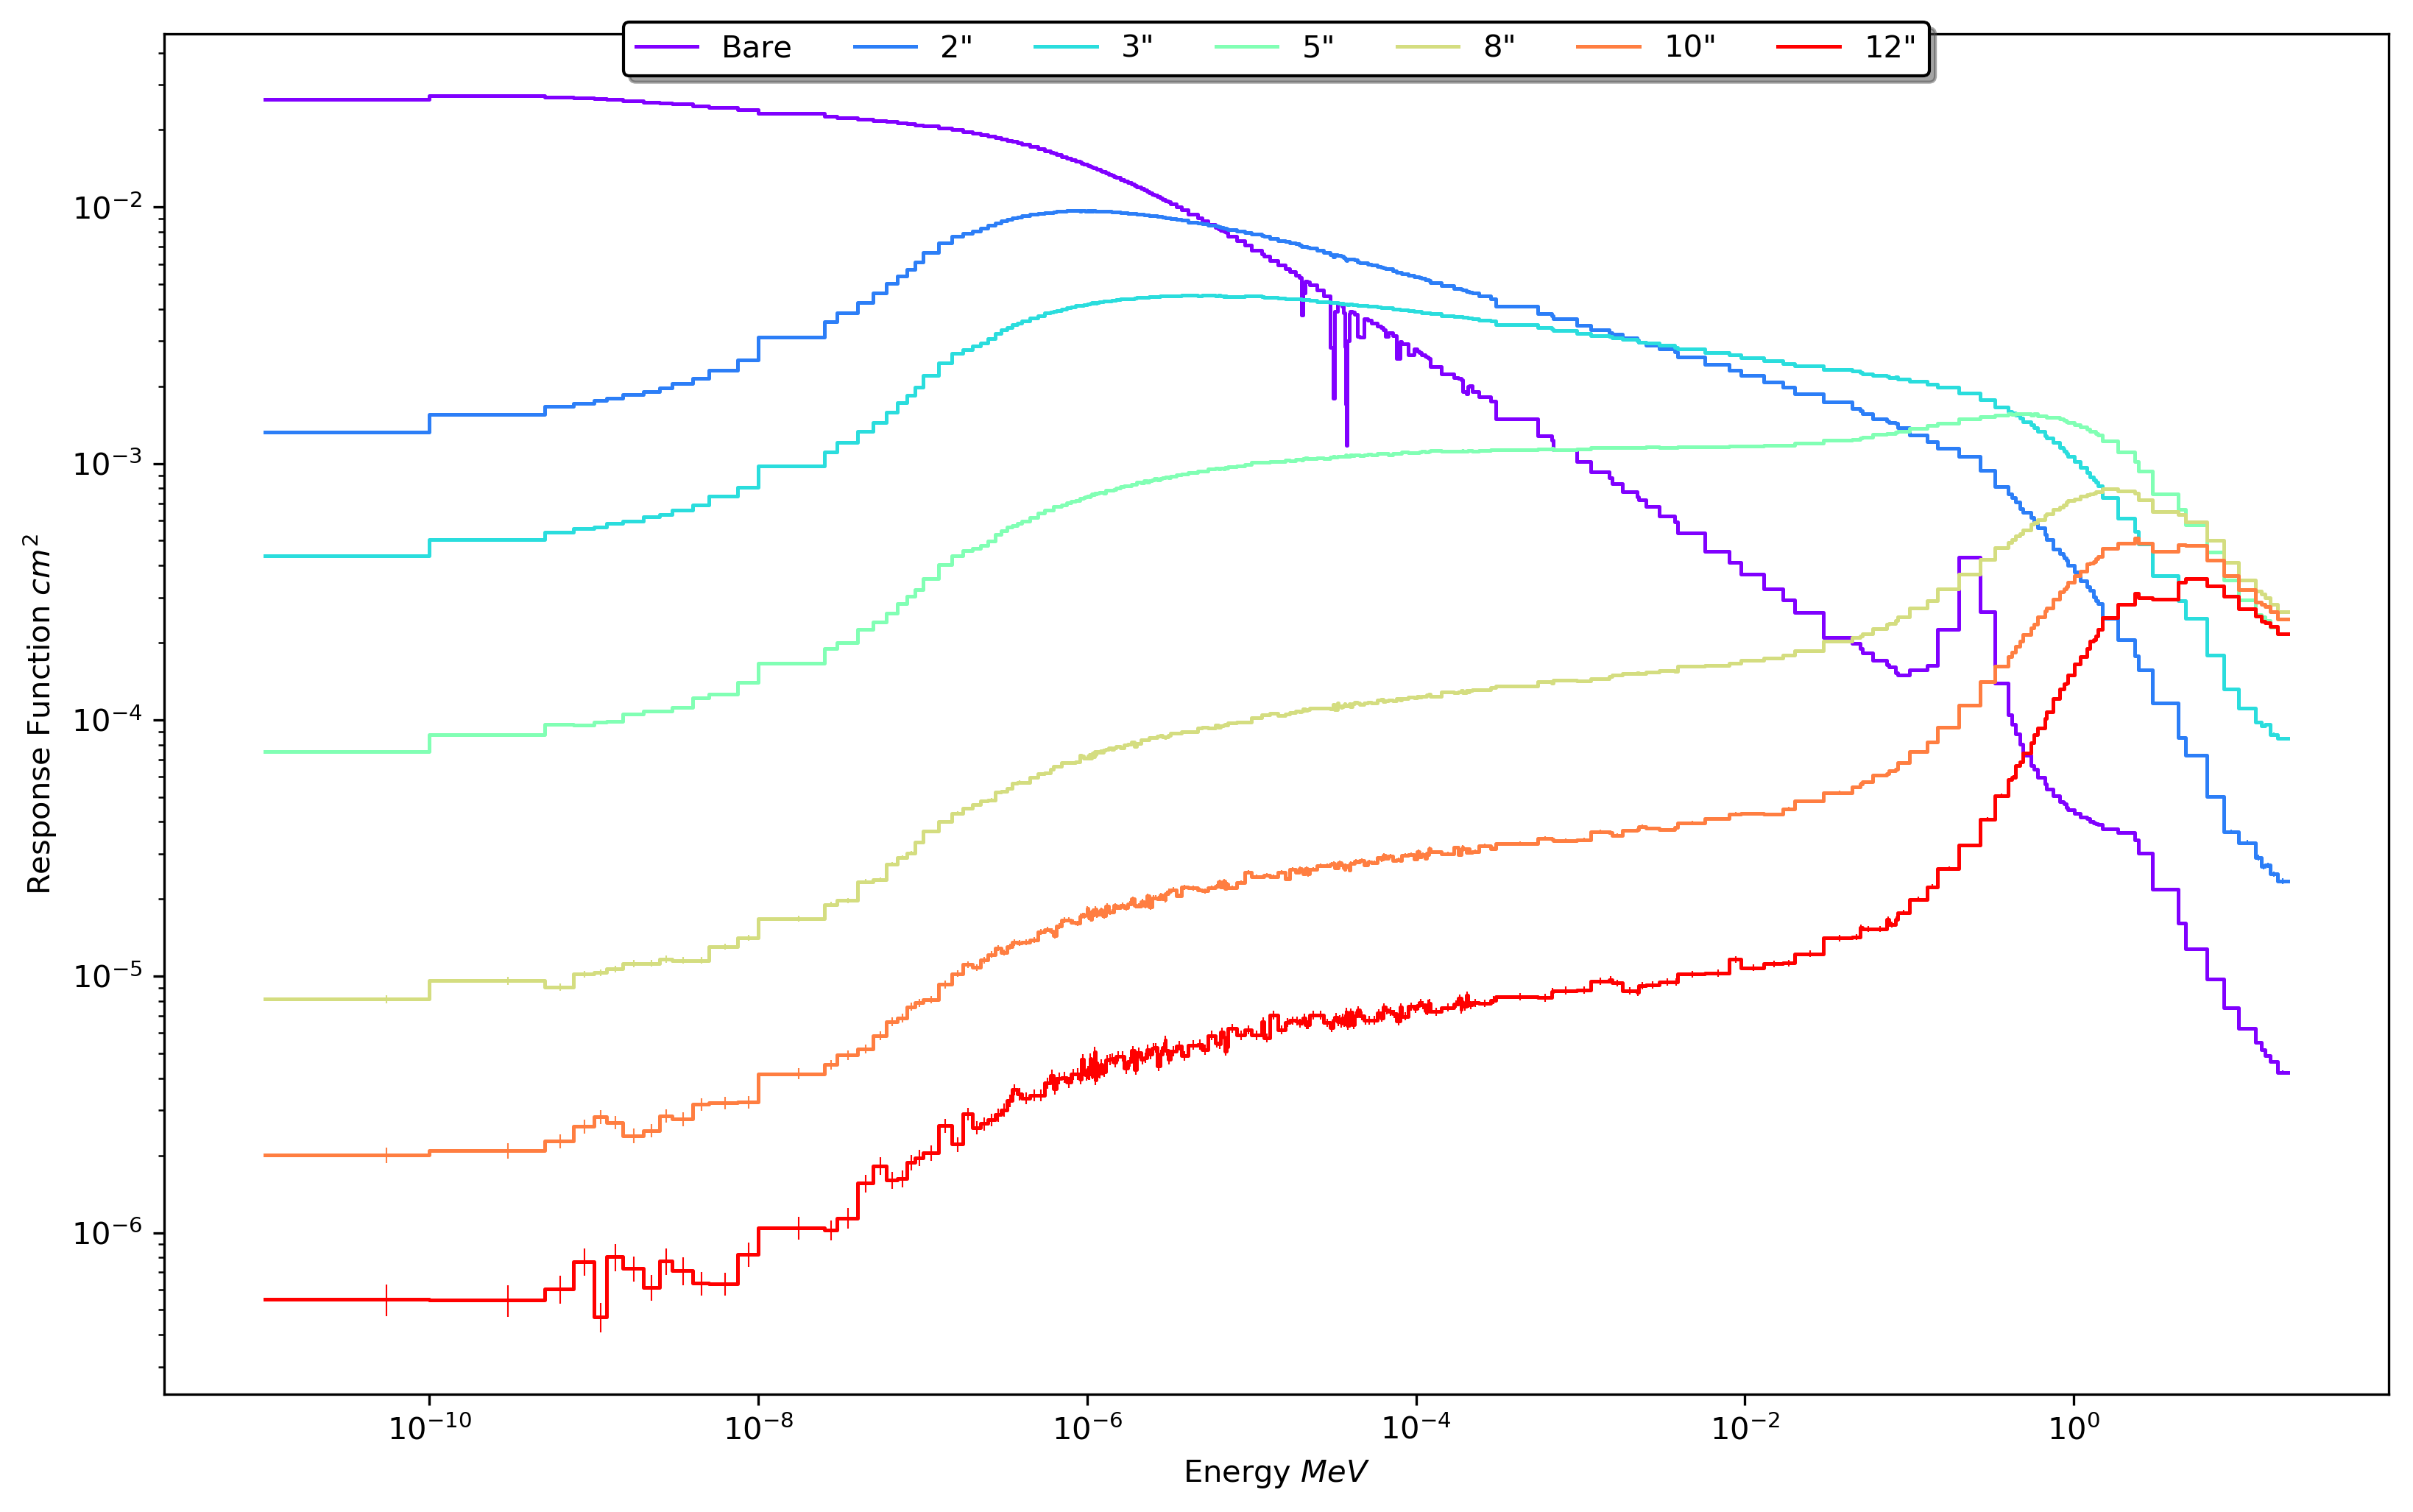
\includegraphics[height=4in]{tex/figures/bs.png}
\caption[Bonner Sphere Spectrometer Response Functions]{The response functions for the Bonner Sphere Spectrometer.}
\label{fig:bs_rfs}
\end{figure}

The trends in the BSS are similar to that of the gold foil tubes.
The bare response is thermally dominated, but as HDPE spheres are added, a peak begins to form and then is pushed towards the right.
The main difference between the two devices, besides number of detectors, is their respective responses to thermal neutrons.
Even though the thermal response is depressed in the gold foil tube, the BSS is almost completely insensitive to thermal neutrons, and there is a much larger difference between the fast and thermal response.
This is likely due to the spherical geometry used.
The BSS have lots of room around the detector for neutrons to thermalize, meaning that the fast peaks will grow to be very sharp.
In the foil tube's case, a scattered neutron is much more likely to escape the device and not be absorbed by the foil, meaning that the contribution to the fast portion of the spectrum will be much lower, relatively.

% -------------------------------------------------------------------------------------------
\section{Experimental Procedures}


\subsection{Gold Foil Tube}

% foils were individually weighed and included in table
First, the foils were individually weighted and those values are shown in \TAB{tab:au_masses}.
% the device was assembled
The device was then assembled as described in the modeling section.
% outer shielding was removed from the beam port configuration
Some of the outer shielding around the beam port was removed to access the collimator.
% the devices was attempted to fit into the beam port but deformation prevented insertion
Initially, an attempt was made to insert the device into the collimator, but deformation in the aluminum portion of the collimator prevented insertion.
% the device was ground down to fit in and inserted to where the first piece was in line with the aperture of the collimator
The first few inches of the device were then ground down with a belt sander to reduce the diameter of the device slightly.
The device was then inserted into the reactor.
% then, the reactor was powered on to __ kwth
Reactor power was brought to 100kW(th).
% the reactor remained at power for __ hours
The reactor remained at power for approximately 2.5 hours.
% then the reactor was shut down
Following the irradiation, the reactor was shut down.
% after allowing the device to cool for a bit, the individual foils were removed and bagged
A cooling period was necessary for the short-lived isotopes produced in the collimator and device to decay.
Then, the device was removed, and from the device, the individual foils were removed and bagged.
% foils were moved to an individual counting station where they were counted (gamma spec)
The foils were moved to an individual counting station, where they were sequentially counted using an HPGE.

% foil tube experimental configuration
\begin{figure}[htb]
\centering
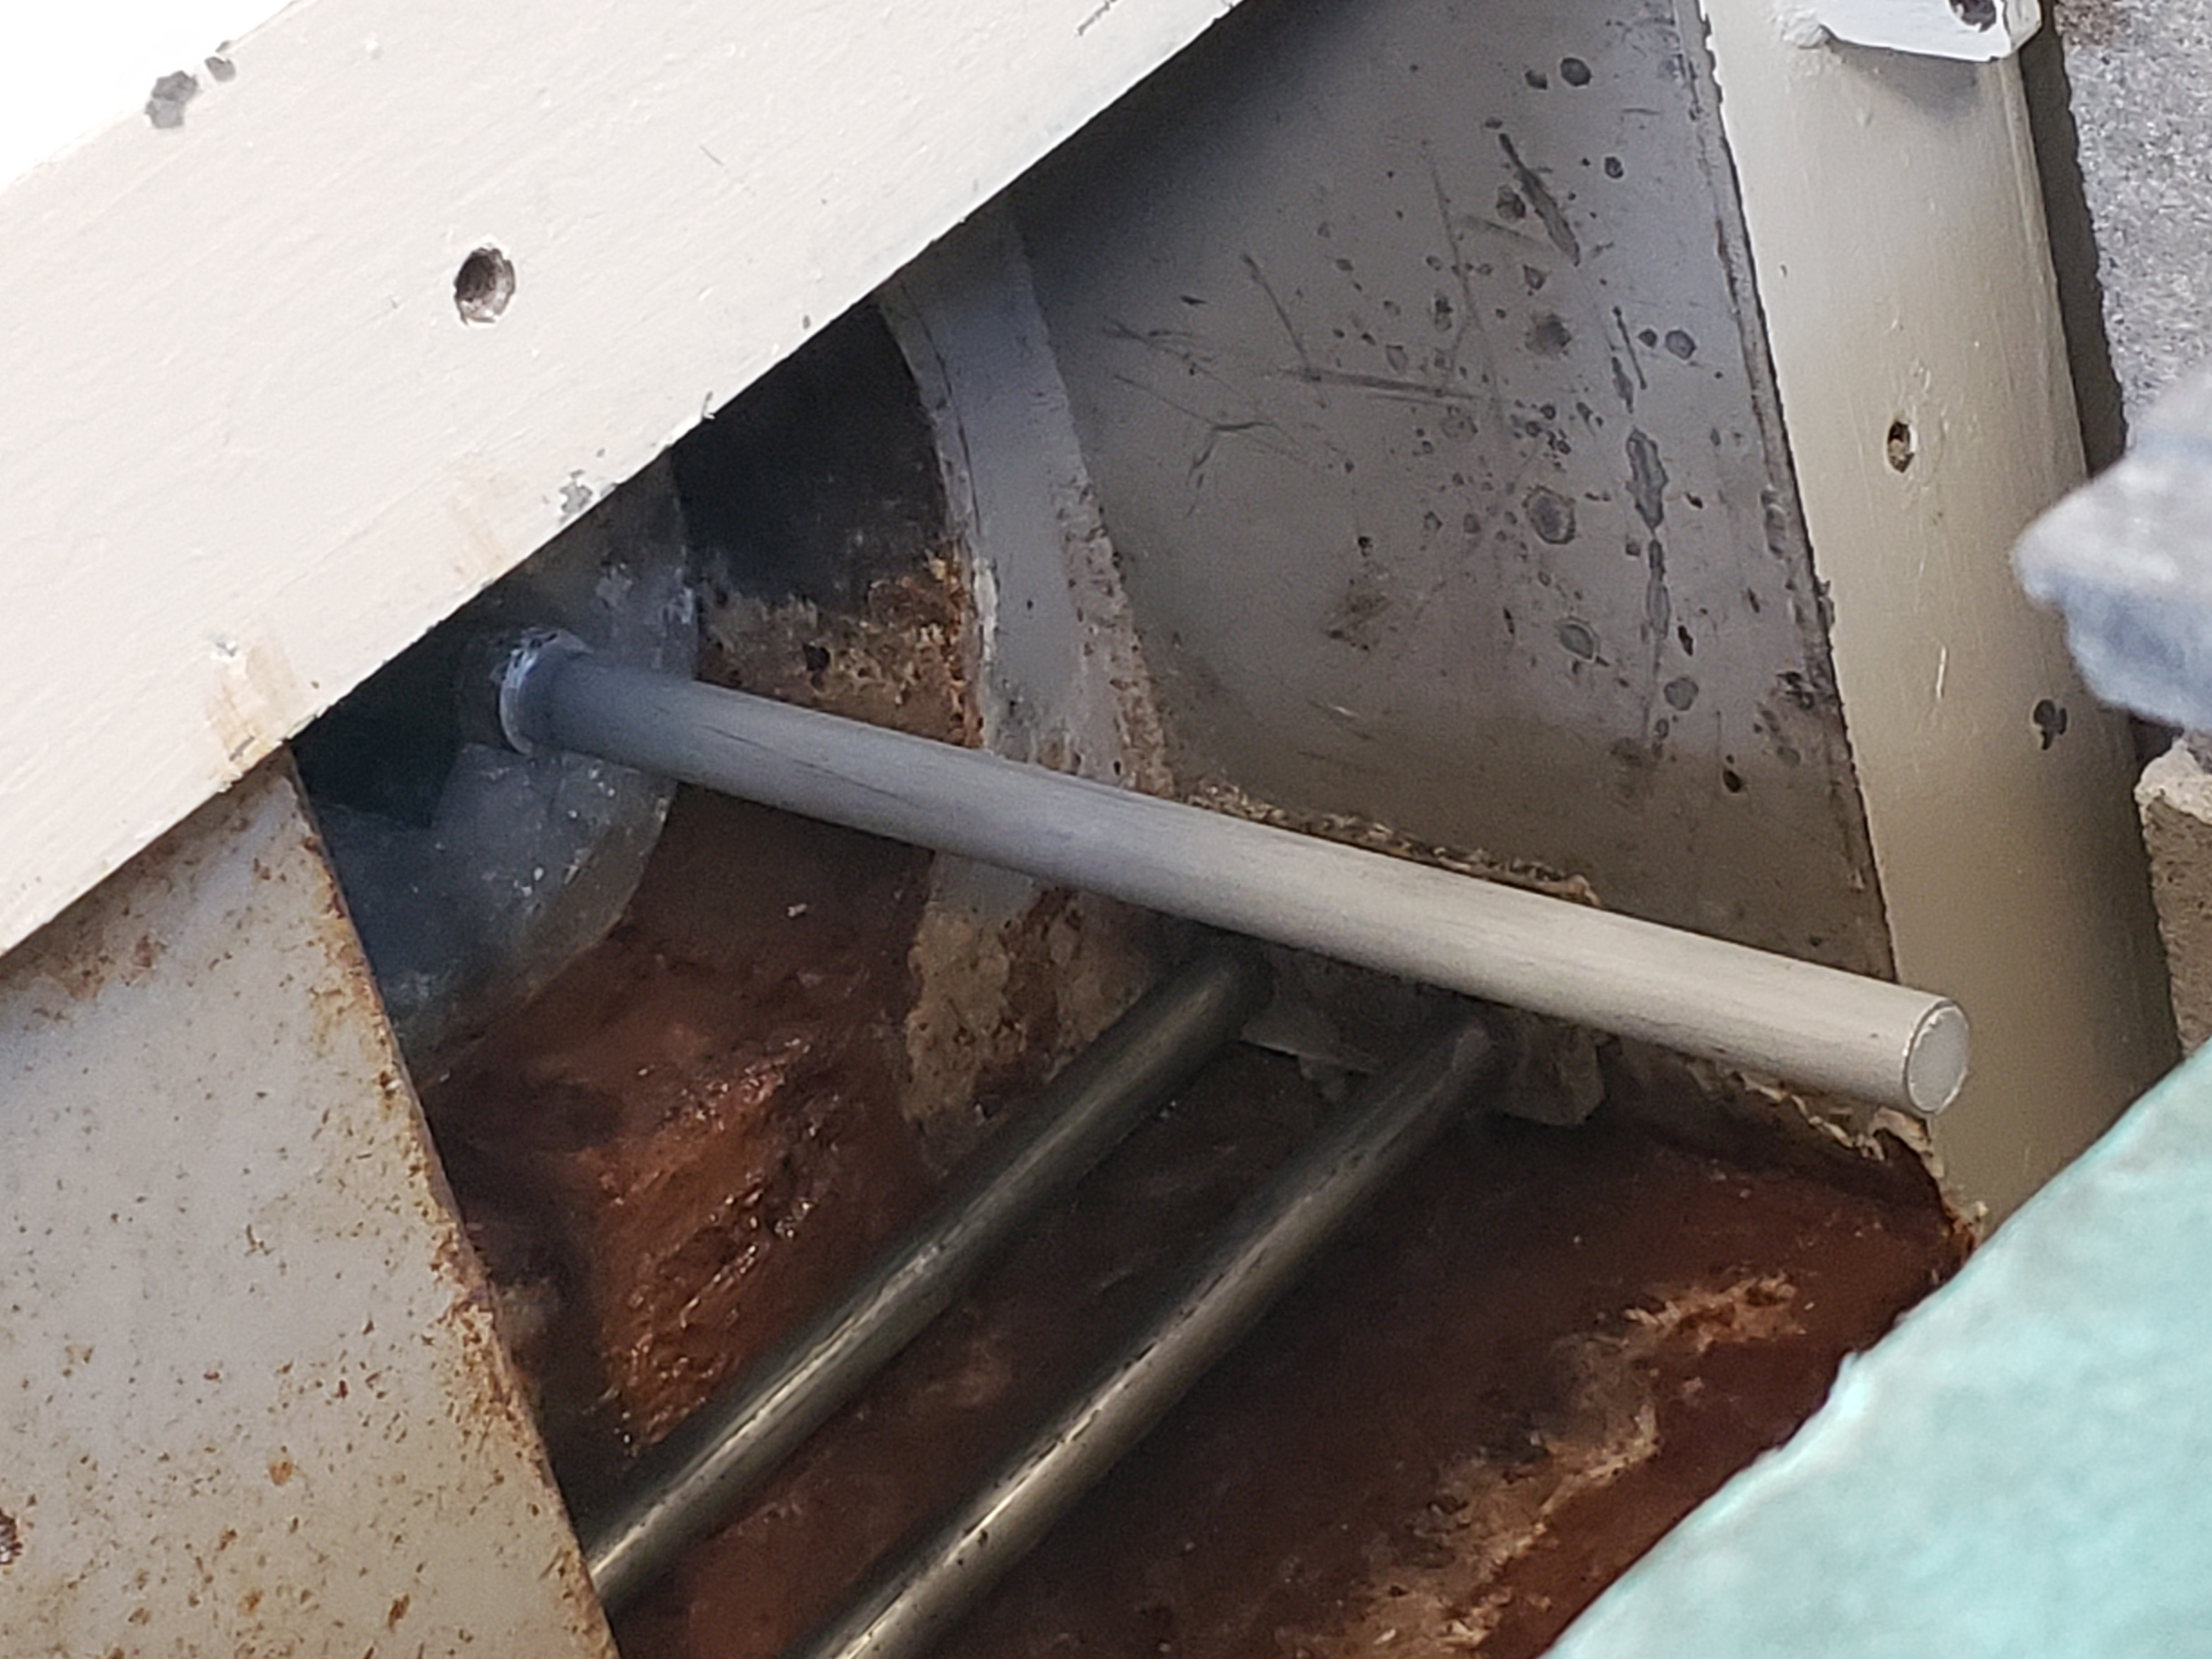
\includegraphics[height=3in]{tex/figures/ft_au_in_beam.jpg}
\caption[Gold Foil Tube Experiment]{A view of the gold foil tube inserted into the NEBP collimator.}
\label{fig:ft_au_in_beam}
\end{figure}

% this contains all of the advantg parameters
\begin{table}[h]\centering
\label{tab:au_masses}
\caption{The masses of the gold foils.}
\begin{tabular}{ r | r | l }
\toprule
Foil ID  & Position (in.)     &   Foil Mass (g)\\
2 & 0 & 0.0320\\
13 & 1 & 0.0312\\
4 & 2 & 0.0320\\
5 & 3 & 0.0318\\
6 & 4 & 0.0319\\
7 & 5 & 0.0325\\
8 & 6 & 0.0326\\
9 & 7 & 0.0320\\
10 & 8 & 0.0318\\
11 & 9 & 0.0326\\
12 & 10 & 0.0317\\
\end{tabular}
\end{table}

\subsection{Bonner Sphere Spectrometer}

% for the bonner spheres, the device was placed vertically in a manner that aligned the detection crystal with the beam at a distance of ___ cm
For the BSS irradiation, the device was positioned vertically in a manner that aligned the detection crystal with the center of the beam at a distance of (???) cm.
% the detector was set to aquire for __ s, and then the reactor was brought to __ kwth.
The detector was set to aquire for 300 s live time and then the reactor was brought to 100kW(th).
% the lld setting was adjusted to where the noise could be removed, but the lithium,T peak wasn't affected
The lld setting was electronically adjusted to reduce the detector dead time, without removing the $^6$Li(n,t) peak.
% spectra were aquired for each configuration
Spectra were aquired for the bare, 2", 3", 5", 8", 10", and 12" configurations.
For the 12" sphere, a live time of 600 seconds was used to help achieve lower counting statistics.
% the reactor was then powered off
Following the experiment, the reactor was powered off.

% ------------
% i need to put all the detection settings and stuff here
% ------------


% ------------
% also, add pictures of both setups
% ------------


% -------------------------------------------------------------------------------------------
\section{Postprocessing and Results}


\subsection{Gold Foil Tube}


% postprocessing includes taking the measured activities and converting them to saturation activities
The postprocessing necessary for a foil activation experiment involves taking the measured activities, which are reported from the gamma spectrometry software, and backing out the saturation activities for each foil.
% this is done using the following equation
This is done using the following equation,

% how to get saturation activities
\begin{equation}
\label{eqn:a_sat}
A_{sat} = A_{meas} \frac{R_{meas}}{R_{sat} n_a K I_{rel}} ,
\end{equation}

% where, (explain these terms)
where $R_{meas}$ is the ratio that corrects for decay during measurement, $R_{sat}$ is the saturation ratio which will be explained below, $n_a$ is the number of sample atoms, equal to $\rho N_A / M$, $K$ is the isotopic abundance, and $I_{rel}$ is the relative intensity of the counted gamma ray.

% give the term and explain for r_meas
The term, $R_{meas}$ is the ratio of the activity at the beginning of the gamma counting to the activity assuming the decay is constant during counting.
It is given by the following equation

% measurement ratio/correction factor
\begin{equation}
\label{eqn:r_meas}
R_{meas} = \frac{\lambda t_{meas}}{1 - e^{\lambda t_{meas}}},
\end{equation}

in which $\lambda$ is the decay constant and $t_{meas}$ is the time during measurement.

% explain the concept of saturation ratio
The saturation ratio, $R_{sat}$, is the ratio between the activity at the time of measurement and the saturation activity.
Although this value generally assumes constant production during irradiation followed by a period of decay with no production, a method has been developed that captures transient behavior in reactor fluxes which will be detailed here.

The production and decay of radioisotopes is expressed mathematically through the bateman equation,

\begin{equation}
\label{eqn:bateman}
\frac{dN(t)}{dt} = C(t) - \lambda N(t)
\end{equation}

where $N(t)$ is the number of radioactive nuclei in the sample, C(t) is the production term in nuclei per second, and $\lambda$ is the decay constant for the isotope in consideration.
The change in radionuclei is simply the production minus the loss.
The relationship between activity and radionuclides, $A(t) = \lambda N(t)$ allows us to convert \EQ{eqn:bateman} into the following,

\begin{equation}
\label{eqn:bateman_activity}
\frac{A(t)}{dt} = \lambda (C(t) - A(t)).
\end{equation}

We can then divide each of the terms by $C_{sat}$ which is the isotopic production at nominal power.
This value is equal to the saturation activity, since the activity at $t = \inf$ for nominal power is equal to the production at that power.

\begin{equation}
\label{eqn:bateman_ratios}
\frac{A(t) / C_{sat}}{dt} = \lambda (\frac{C(t)}{C_{sat}} - \frac{A(t)}{C_{sat}})
\end{equation}

Two facts allow us to simplify \EQ{eqn:bateman_ratios} into a useful form.
First, because $A_{sat} = C_{sat}$, any $A(t) / C_{sat} = A(t) / A_{sat}$, so we can replace these terms with a defined term, $R_{sat}(t)$ which is the ratio of the activity at time $t$ to the saturation activity.
Second, although we don't have access to the $C(t)$ or $C_{sat}$ terms since they require the (currently unknown) flux, we do have access to power data.
Because isotopic production is approximately proportional to reactor power, $C(t) \propto P(t)$, this means that $C(t) / C_{sat} \approx P(t) / P_{nominal}$.
We will replace this power ratio with the term $P_{f}(t)$, which is simply the time dependent ratio of the power to the nominal power.

\begin{equation}
\label{eqn:bateman_r_sat}
\frac{R_{sat}(t)}{dt} = \lambda (P_{f}(t) - R_{sat}(t))
\end{equation}

This equation can be solved to find $R_{sat}$ at the time of measurement using a numerical solver, in our case, {\tt scipy}'s {\tt odeint}.
The data for $P_{f}(t)$ is simply normalized strip chart data collected from an in-core fission chamber.


% ---------------------
% fix this table later
% ---------------------

% this contains all of the correction factors and foil activities
\begin{table}[h]\centering
\label{tab:a_sat}
\caption{The correction factors and foil activities.}
\begin{tabular}{ r | r | r | l | r }
\toprule
Position (in.)  & $A_{meas}$ (Bq) & $R_{meas}$  & $R_{sat}$   &   $A_{sat}$  (Bq)\\
0 & 1483.73 & 1.00089 & 0.02268 & 65468.28 \\
1 & 58.60 & 1.00590 & 0.02262 &  2605.89  \\
2 & 8.92 & 1.03805 & 0.02196 &   422.02  \\
3 & 4.06 & 1.06581 & 0.0204  &   212.01  \\
4 & 2.58 & 1.14023 & 0.01574  &   186.96  \\
5 & 1.60 & 1.27976 & 0.01340 &      153.12  \\
6 & 0.72 & 1.26894 & 0.00794 &       115.22  \\
7 & 0.37 & 1.27340 & 0.00483 &      97.03   \\
8 & 0.17 & 1.41587 & 0.00256 &       95.65\\
\end{tabular}
\end{table}

% foil responses
\begin{figure}[htb]
\centering
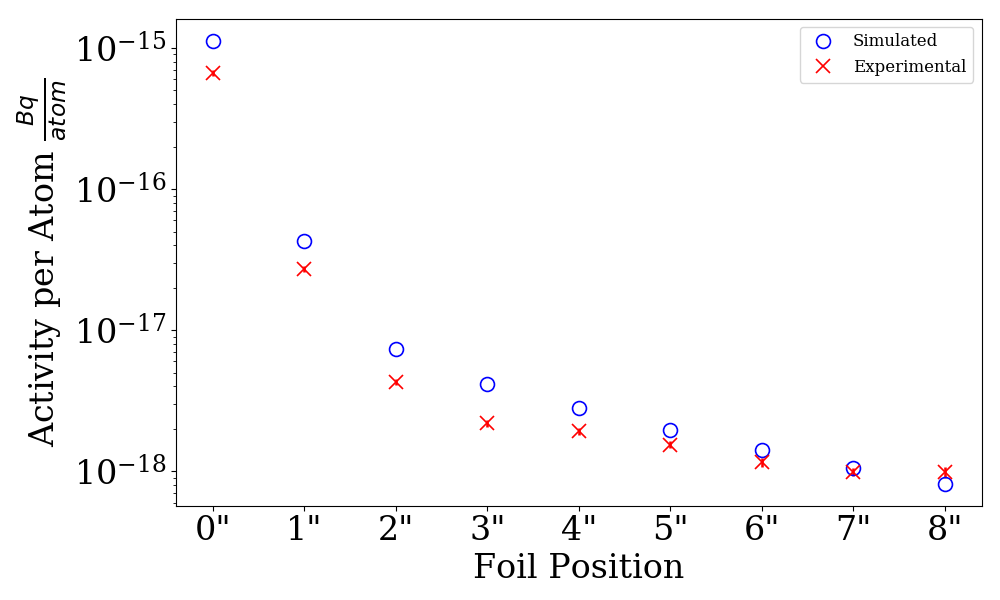
\includegraphics[height=3in]{tex/figures/compare_activities.png}
\caption[Foil Activities]{A comparison of the simulated and experimentally obtained foil activities.}
\label{fig:compare_activities}
\end{figure}


\subsection{Bonner Sphere Spectrometer}

The BSS data was processed simply by taking the area under the LiI reaction peaks and dividing that value by the live time of the detector.
These values are presented in \TAB{tab:bss}.

% bss response integration
\begin{figure}[htb]
\centering
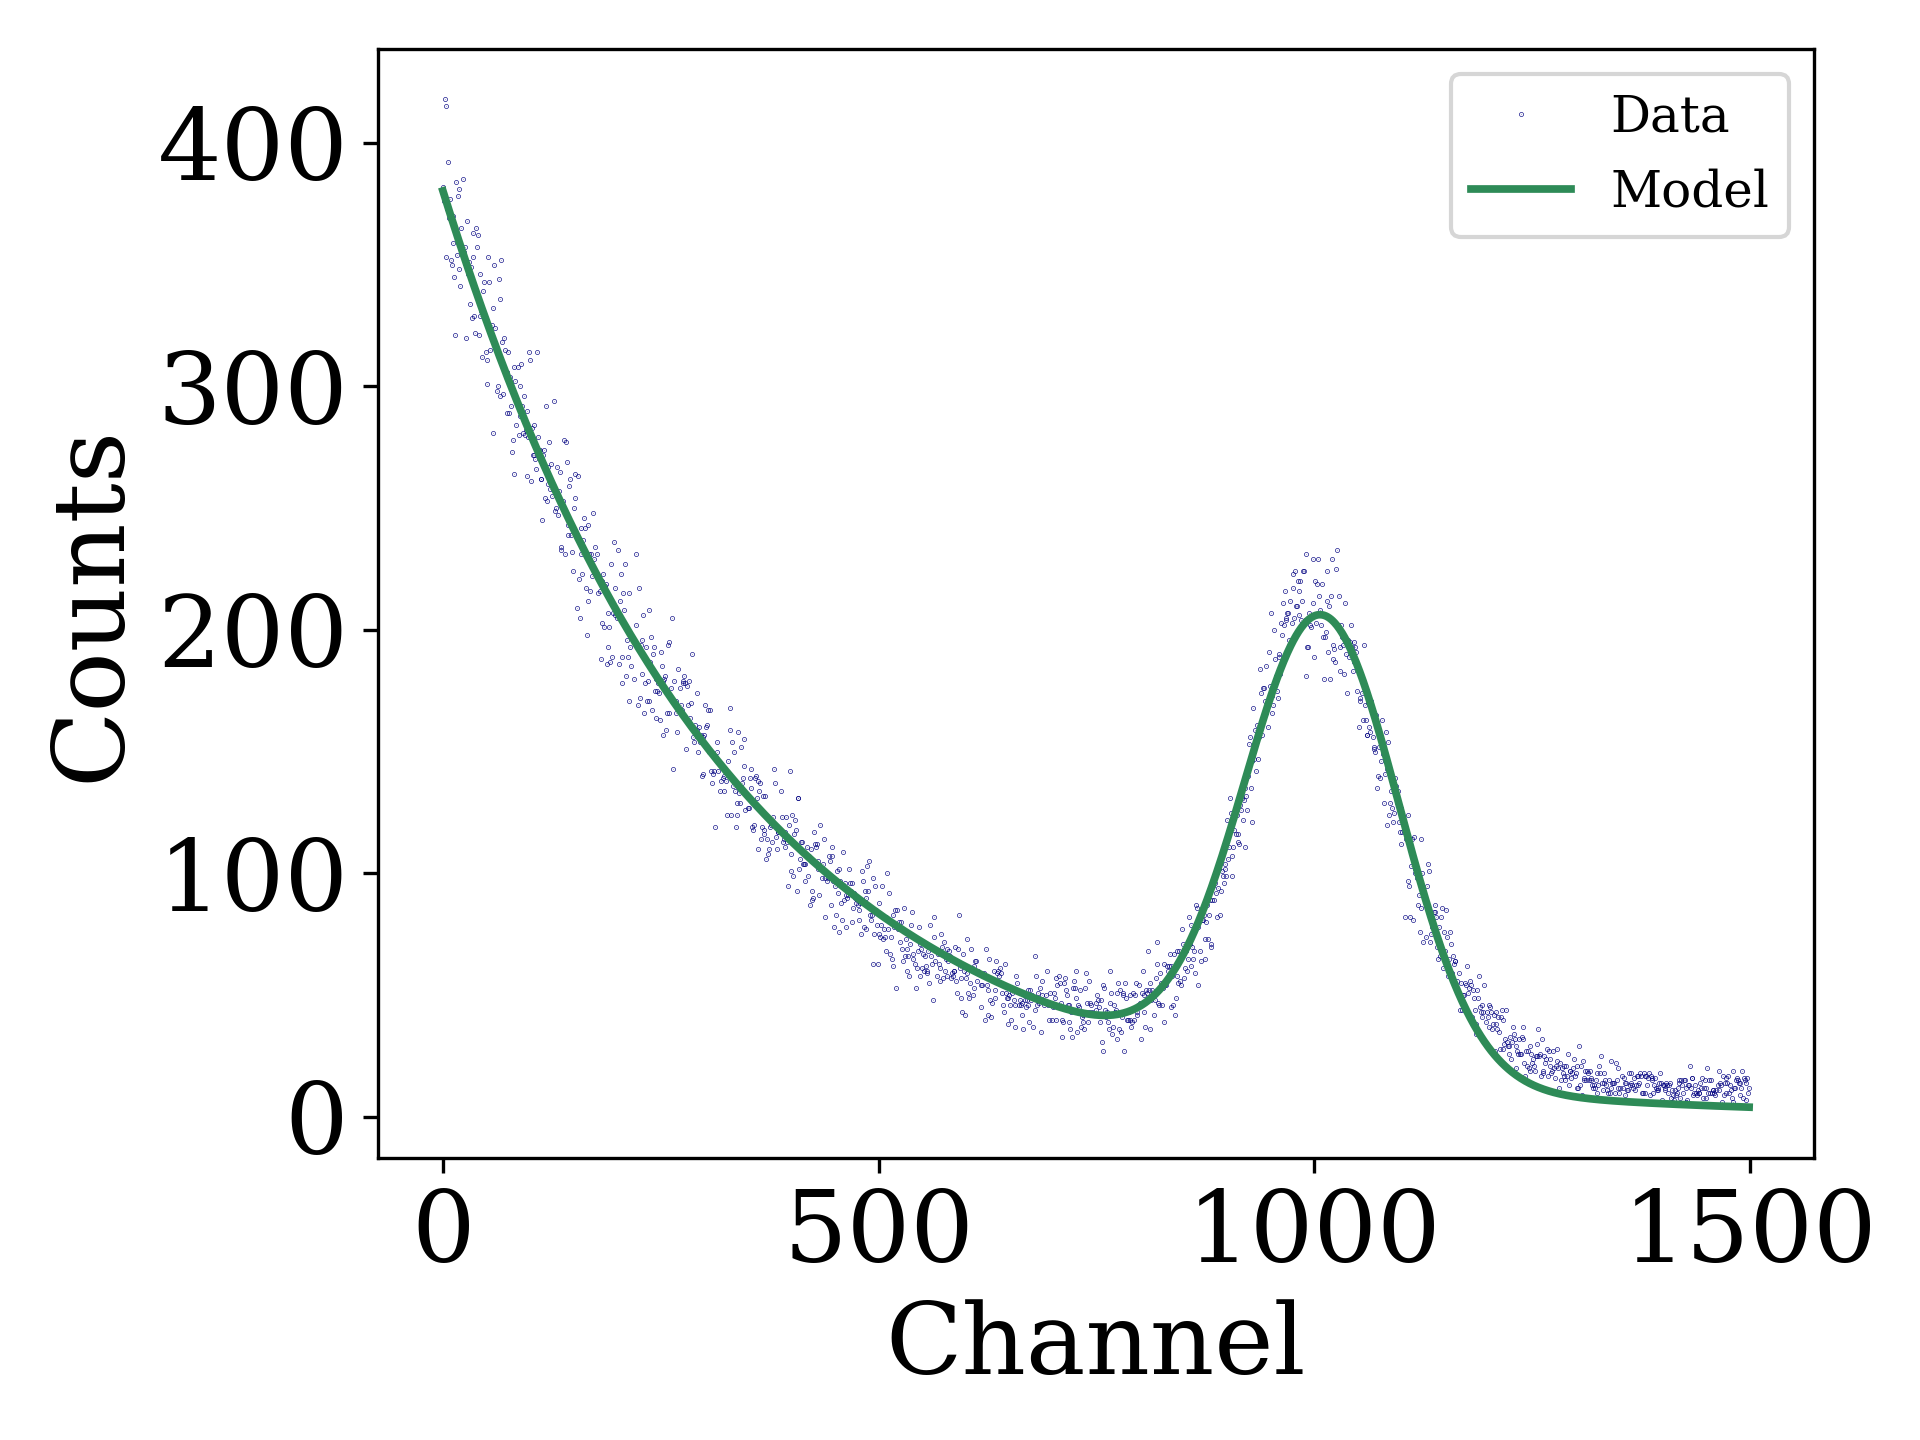
\includegraphics[height=3in]{tex/figures/bs4_spectrum.png}
\caption[8" BSS Spectrum]{The 8" sphere's gamma-ray spectrum and the model used to find the integral response.}
\label{fig:compare_countrates}
\end{figure}


% the bss count rates
\begin{table}[h]\centering
\label{tab:bss}
\caption{The BSS count rates from the experiment.}
\begin{tabular}{ r | r }
\toprule
Sphere (in.)  & Count Rate $s^{-1}$\\
Bare & 1626.76\\
2  & 1062.40\\
3 & 3891.13\\
5 & 417.24\\
8 & 139.72\\
10 & 70.75\\
12 & 37.43\\
\end{tabular}
\end{table}

% bss responses
\begin{figure}[htb]
\centering
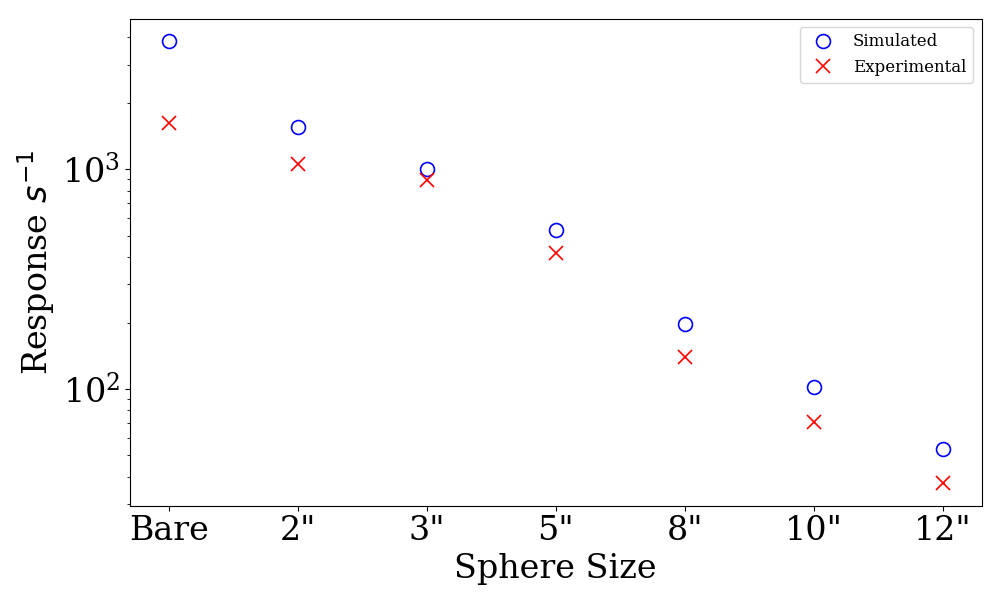
\includegraphics[height=3in]{tex/figures/compare_countrates.png}
\caption[BSS Responses]{A comparison of the simulated and experimentally obtained BSS responses.}
\label{fig:compare_countrates}
\end{figure}


% -------------------------------------------------------------------------------------------
\section{Spectral Unfolding}

\subsection{Methods and Parameters}

% the responses and response functions were used with the unfolding methods described in ch2 to obtain solution spectra
The detector responses and response functions were unfolded with the methods described in chapter two to obtain a set of solution spectra.
% the bss and ft_au results were first considered separately, then combined
The responses from the foil tube and the BSS were first considered separetely, then combined into a single vector to produce a third spectrum for each unfolding method.
% both the gravel and maxed unfolding algorithms were used with these data
The Gravel, Doroshenko, and MAXED unfolding algorithms were used.
% for gravel, 50 iterations were used
For both Gravel and Doroshenko, the termination criteria was set at 50 iterations.
% for maxed, the parameter omega was set using the number of detectors for each dataset, 9 for the foil tube, 7 for the bss, and 16 for the combined set
For MAXED, the parameter Omega was set using the number of detectors for each dataset, 9 for the foil tube, 7 for the BSS, and 16 for the combined case.
% then, the maxed portion was repeated, while first scaling the default spectrum
Then, the MAXED unfolding was repeated, but with a scaled default spectrum.
In this case, scaled means that the default spectrum was normalized so the average of the computed responses was equal to the average of the experimentally obtained responses before unfolding.

\subsection{Results and Discussion}


\begin{figure}[htb]
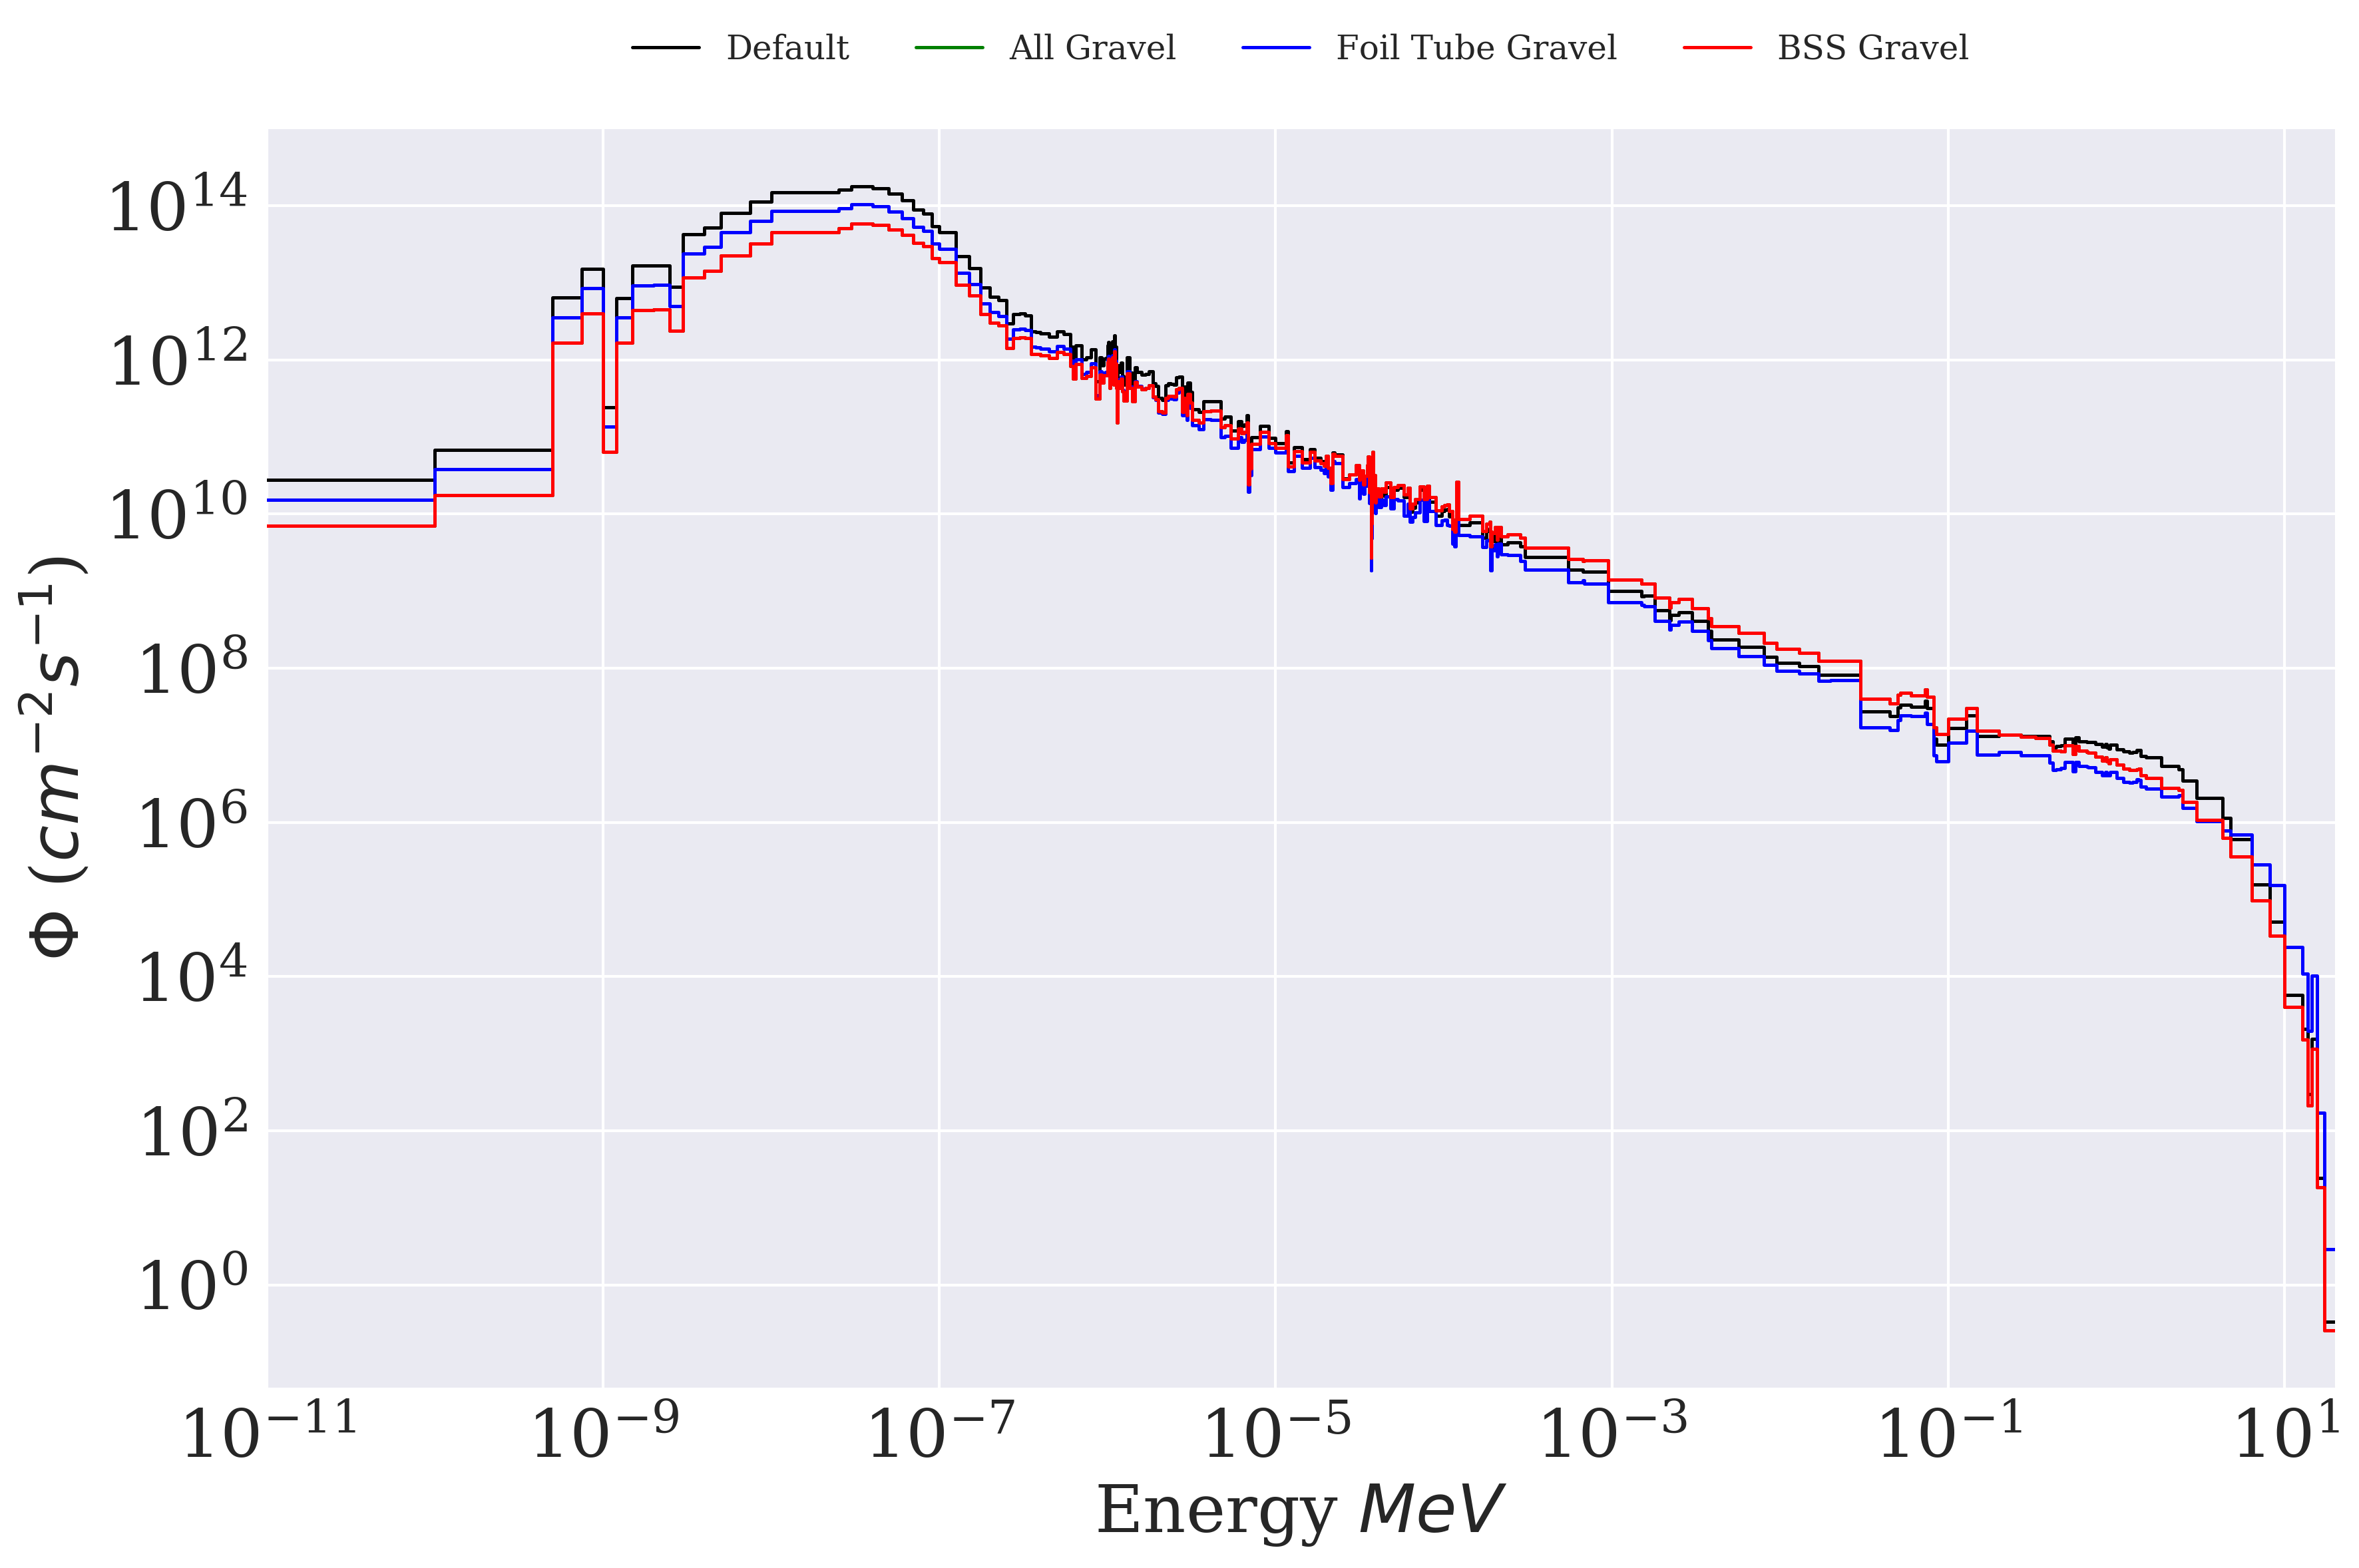
\includegraphics[height=3.8in]{tex/figures/unfolded_gr.png}
\caption[Gravel Unfolded Spectra]{The unfolded NEBP spectra obtained from using the Gravel method.}
\label{fig:unfolded_gr}
\end{figure}

% here gravel results are presented first
Here, the Gravel results are presented in \FIG{fig:unfolded_gr}
% as seen in the figure, the bss and ft_au results show good agreeance with one another
As seen in the figure, the foil tube and BSS results show good agreeace with one another.
% all of the major features from the default spectrum are preserved
All of the major features from the default spectrum are preserved.
% the ft_au results unfold to a slightly higher thermal flux than the bss where as the bss show slightly higher fast region
Some differences appear between the two datasets, where the foil tube shows a slightly higher thermal flux and the BSS is larger through a portion of the fast region.
% the combined results cannot be seen as they are covered by the ft_au
The combined results cannot be seen as they are covered by the foil tube data.
% this is because with gravel, smaller error responses are weighted heavier and the errors are much smaller for the gold foils than for the bss
This is due to the fact that the gravel algorithm will base its manipulation on relative error, meaning that smaller error (more well-known) responses will affect the final results more, and the errors from the foil tube are much smaller than the BSS results.

\begin{figure}[htb]
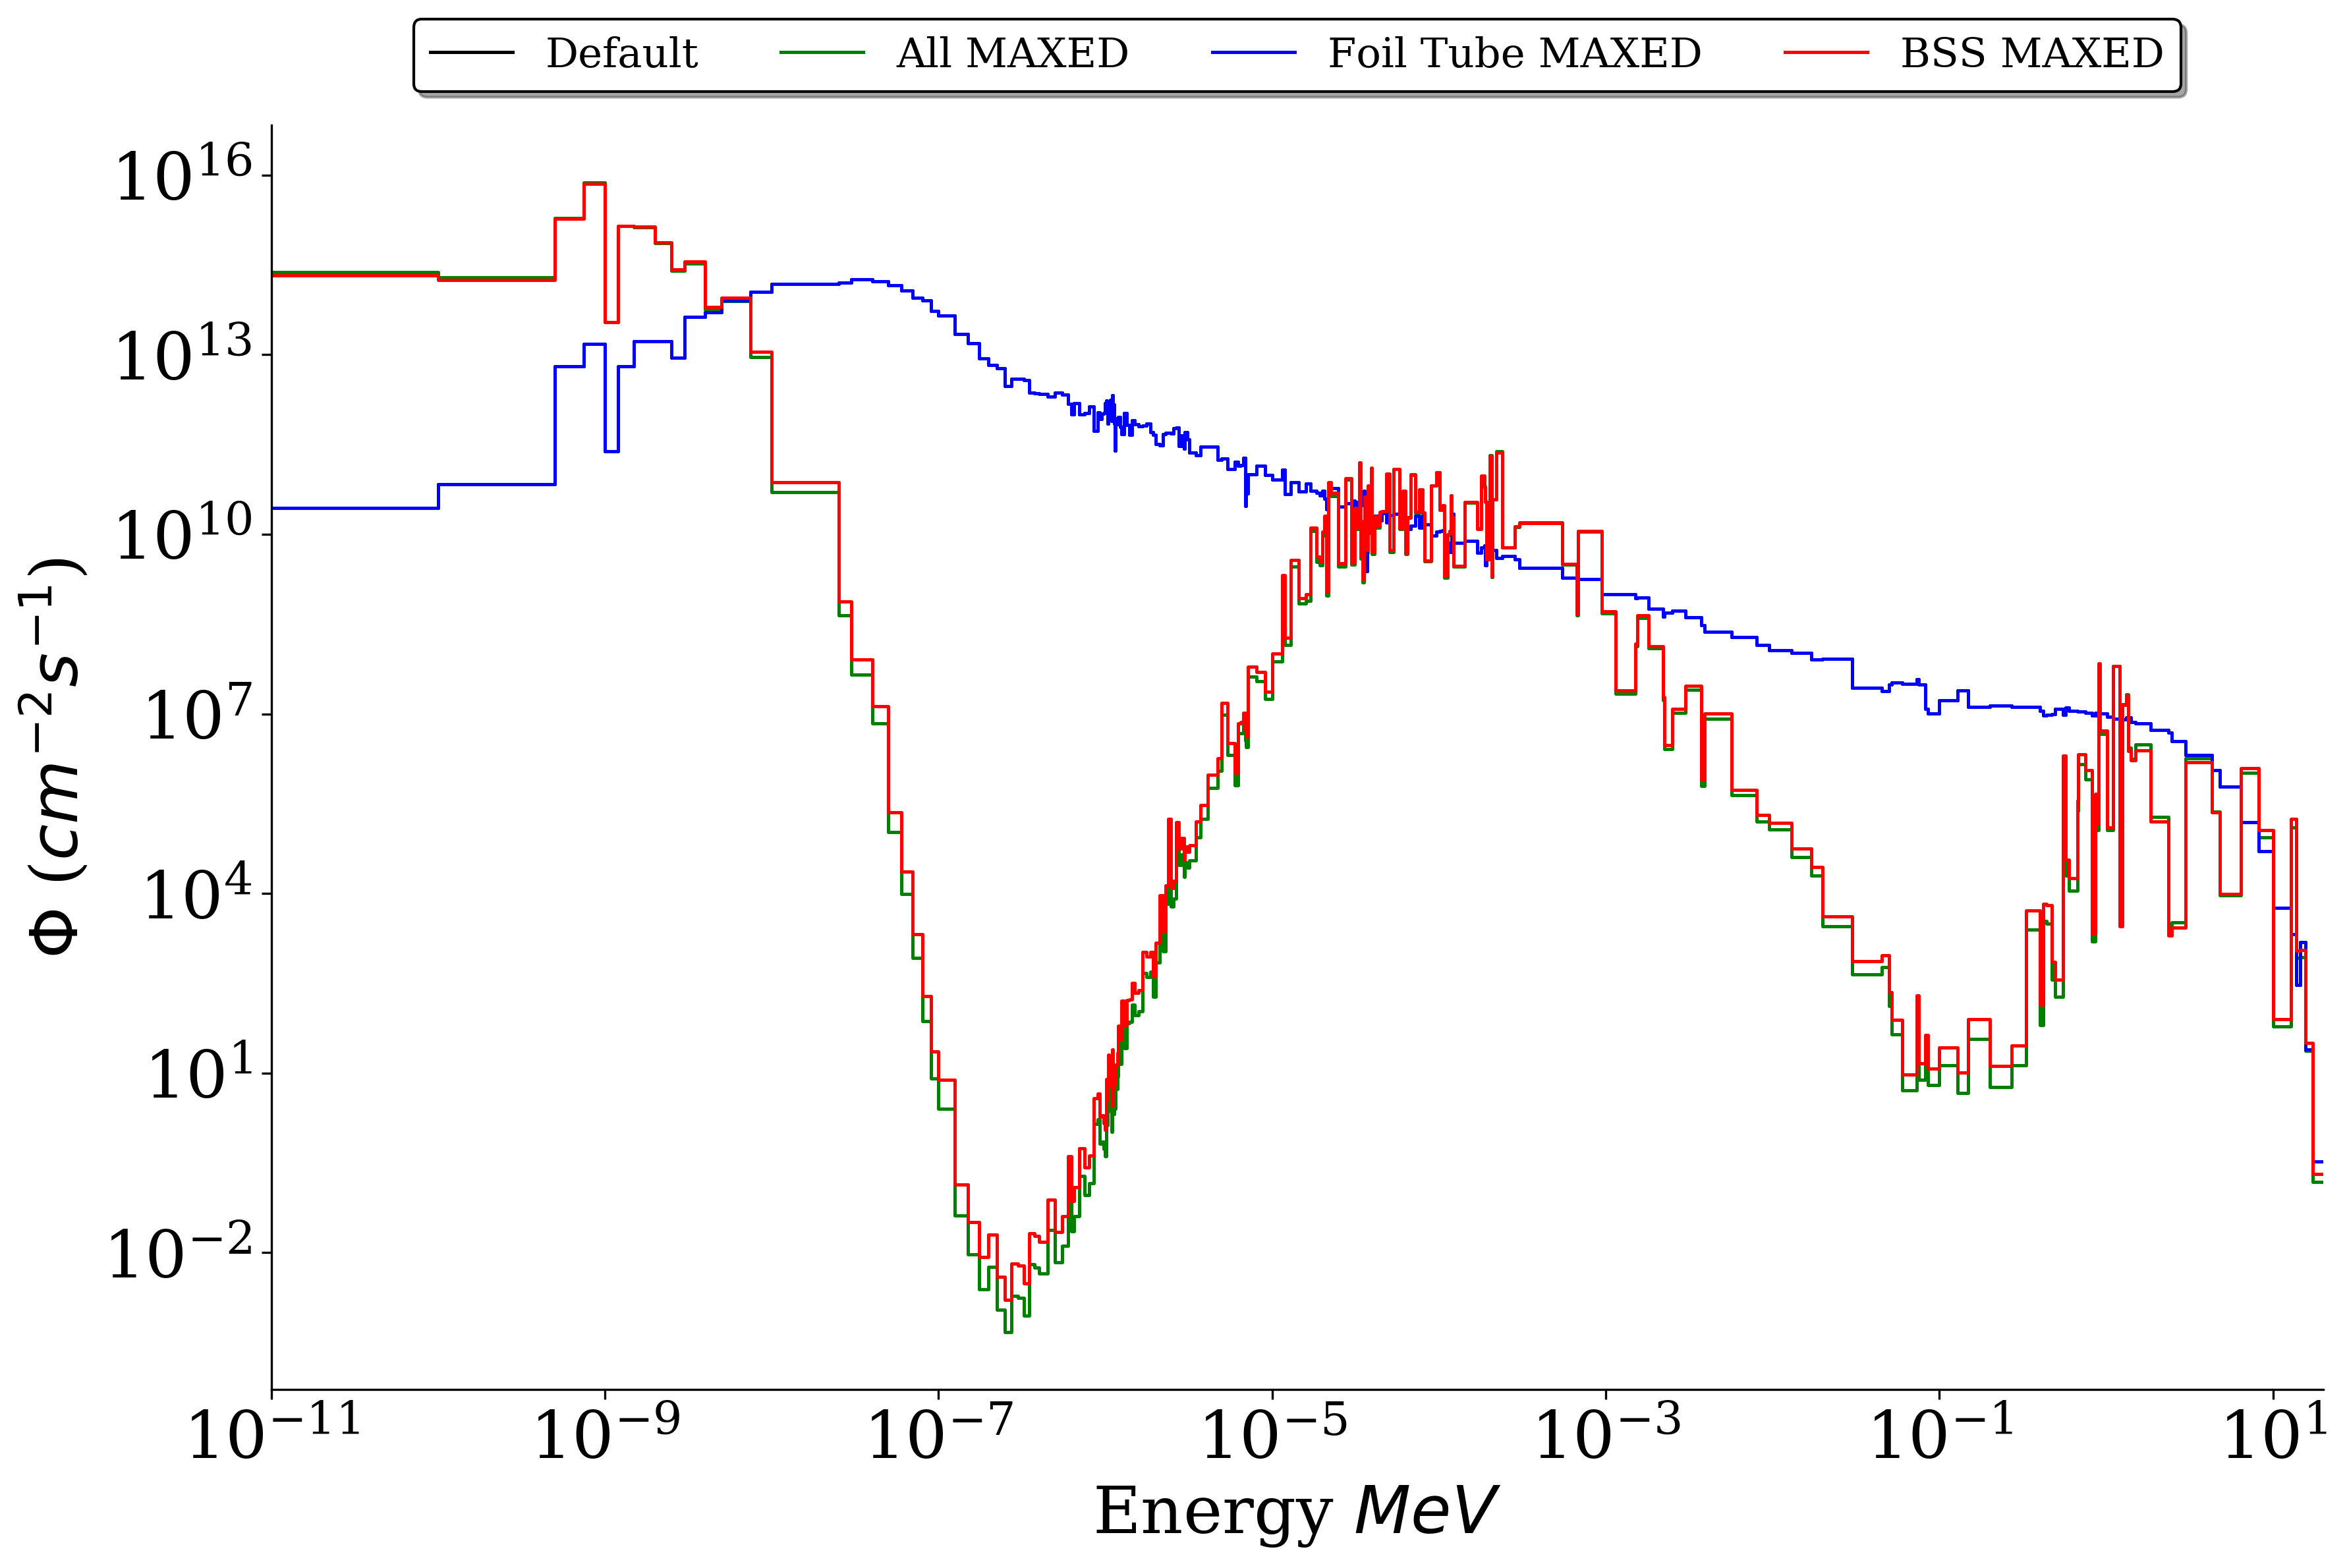
\includegraphics[height=3.8in]{tex/figures/unfolded_mx.png}
\caption[MAXED Unfolded Spectra]{The unfolded NEBP spectra obtained using the MAXED method.}
\label{fig:unfolded_mx}
\end{figure}

% these results shown in FIG are from the maxed unfolding.
Seen in \FIG{fig:unfolded_mx} are the results from the MAXED unfolding.
% in the case of the bss and combined case, the results produced are very unphysical
In the BSS and combined cases, the results produced appear very unphysical.
% this is likely due to the fact that the spectrum is trying to fit the data while staying close to the default spectrum
This is likely due to the fact that the algorithm is trying to fit the data while retaining some values close to the defaults spectrum to maximize the cross entropy between the two spectra.
% in the ft_au case, the default spectrum remains unchanged, indicating that the default spectrum actually represents a decent fit of the data
The default spectrum remains unchanged for the foil tube case, which indicates that the default spectrum actually represents a decent fit of the data, although it's still not as close as in the Gravel case.

\begin{figure}[htb]
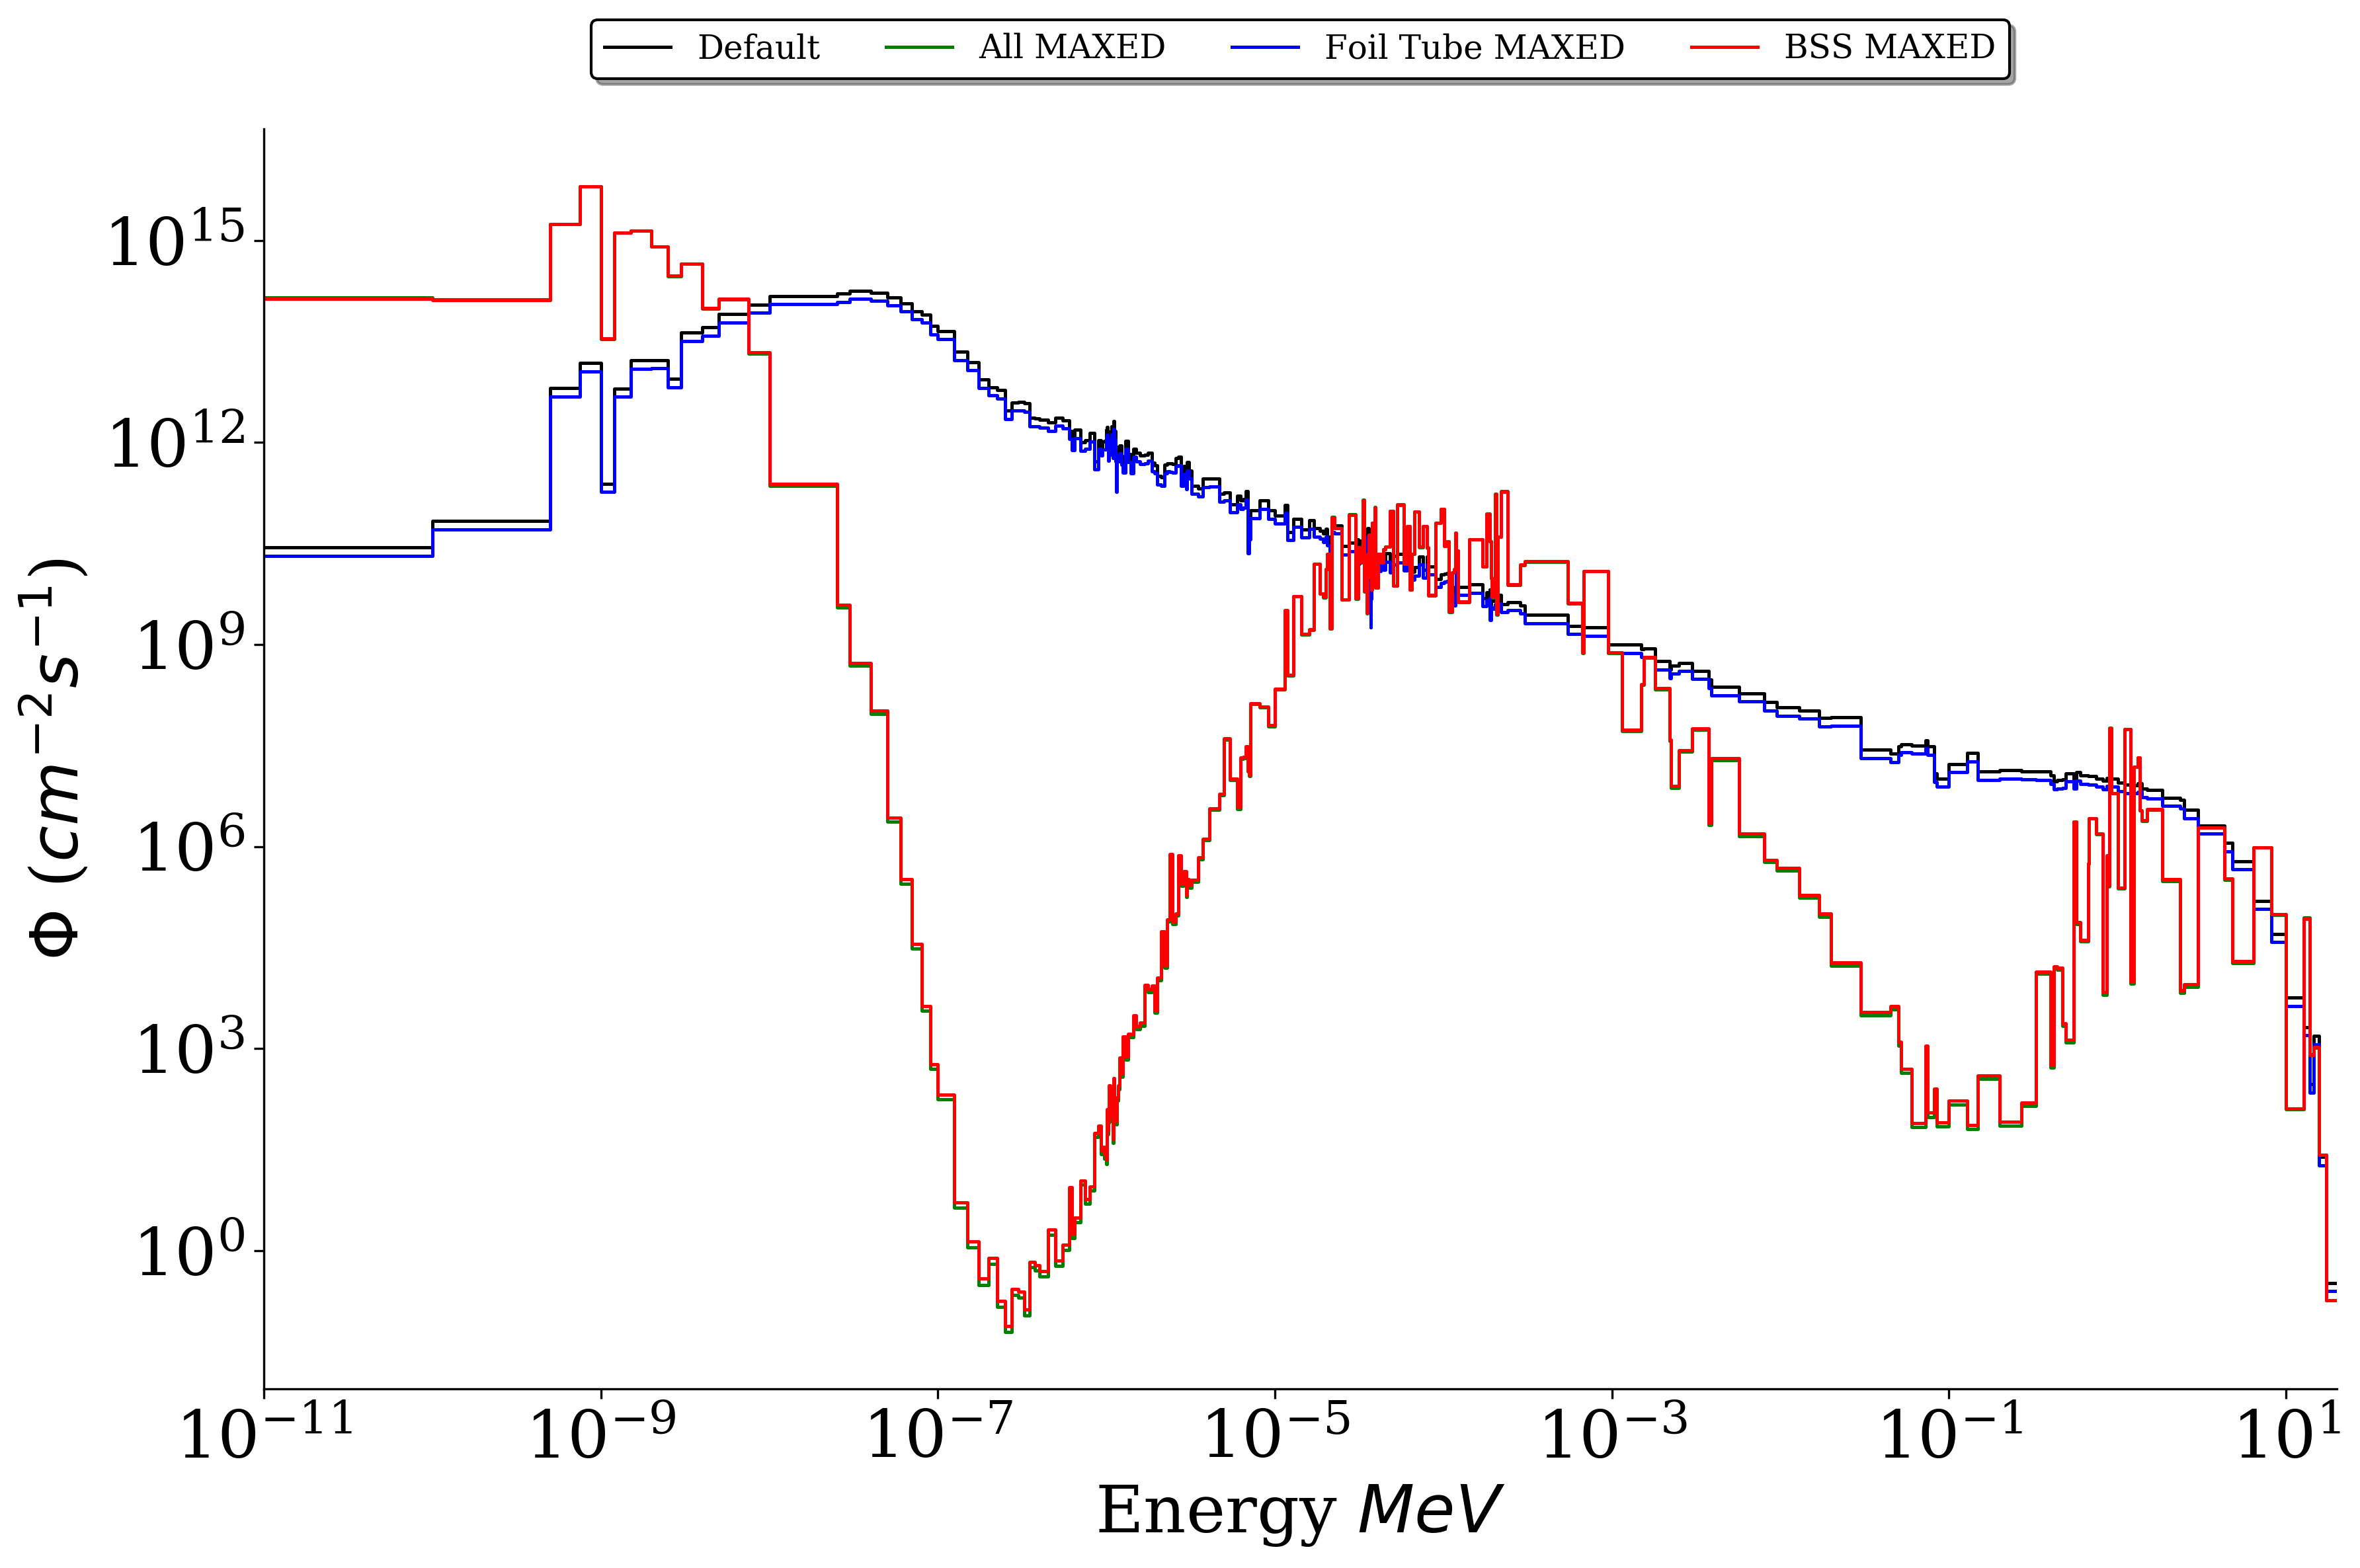
\includegraphics[height=3.8in]{tex/figures/unfolded_mx_sc.png}
\caption[MAXED Unfolded Spectra (Scaled)]{The unfolded NEBP spectra obtained from scaling the default spectrum then unfolding with the MAXED method.}
\label{fig:unfolded_mx_sc}
\end{figure}

% although it was hypothesized that scaling the spectrum would results in a less erratic answer, the results here are very similar in characteristics to the unscaled maxed results
It was hypothesized that scaling the defaults spectrum would remove some of the unphysicalities of the solution spectra; however, the results in \FIG{fig:unfolded_mx_sc} still appear erratic and are very similar in characteristics to the unscaled versions.
% the bss and combined cases are still unphysical, and the ft_au remaines unperturbed
The BSS and combined cases are still rather unphysical, and the foil tube solution remains unperturbed.

\begin{figure}[htb]
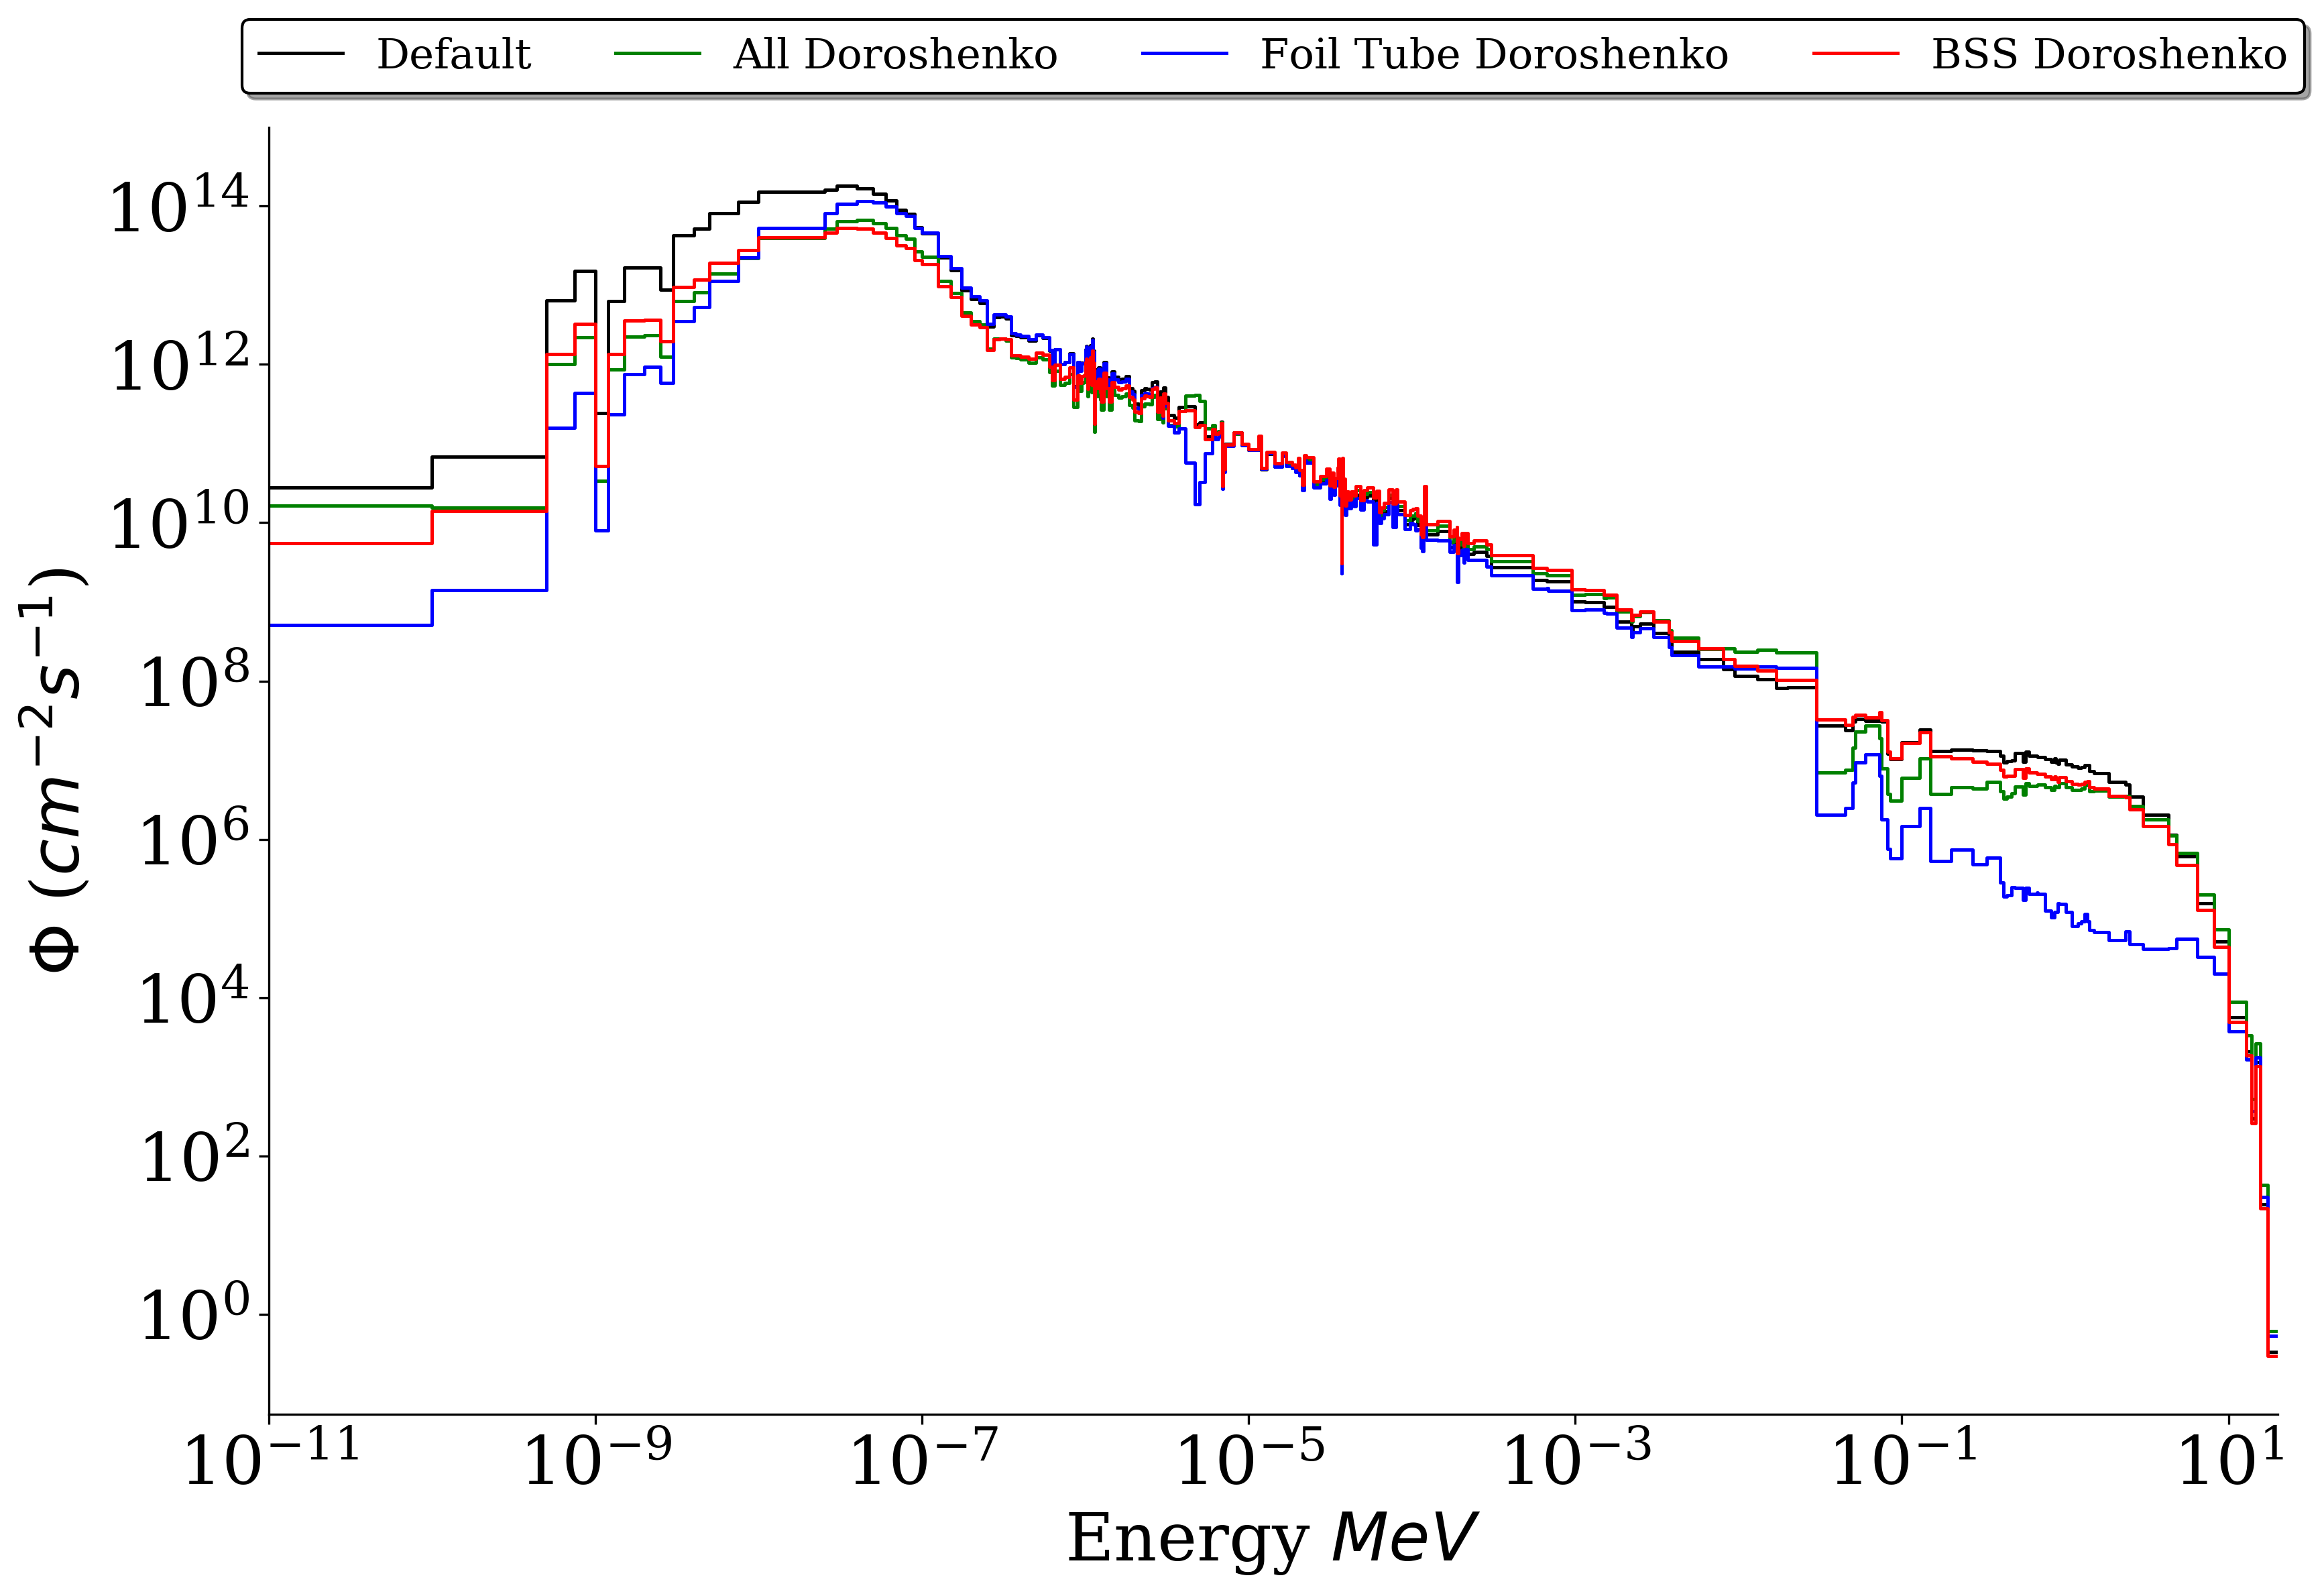
\includegraphics[height=3.8in]{tex/figures/unfolded_do.png}
\caption[Doroshenko Unfolded Spectra]{The unfolded NEBP spectra obtained from unfolding with the Doroshenko method.}
\label{fig:unfolded_do}
\end{figure}

% results in figure are from doroshenko
The results in \FIG{fig:unfolded_do} are from the Doroshenko unfolding.
% unlike maxed, they appear similar to the unfolding with gravel
Unlike MAXED, these results appear stable, like the Gravel data.
% here, though, the differences in the datasets are exemplified
Here, though, the differences between the datasets are more exemplefied.
This is most obvious in the foil tube dataset.
The fast end of the spectrum appears flattened as it tries to fit some of the foil data whose responses lie in that end.
Those responses have high error and likely this feature is due to a bias in the measurement, and not an actual spectral feature.
The other two datasets unfolded into reasonable-appearing spectra, with some slight variation in both the center of the maxwellian distribution, as well as in the flatness of the fast region.




\cleardoublepage


\chapter{Conclusions and Future Work}

\section{Conclusions}
%% concise statements about your main findings, related to your aims/objectives/hypothesis.
% it's possible to simulate the beam w/ advantg
First, through the assistance of the VR methods described, it is possible to find the neutron spectrum for a collimated reactor beam port.
% a high resolution flux was obtained via simulation
A high resolution flux spectrum was obtained via Monte Carlo simulation for the KSU TRIGA Mark II's Northeast Beam Port featuring dimensional data in energy, angle, and the radial direction.
% two separate experiments showed data that agreed with the shape of the simulation work and showed similar magnitude differences
Two separate experiments were conducted which collected data that demonstrated decent shape-agreeance with the simulated spectrum and differed in magnitude from the simulated work by similar values.
% the foil tube was novel
Of the two experiments, one involved the creation of a novel type of neutron spectrometer which solved issues like beam alignment and allowed for several different responses to be obtained using only one irradiation and one type of foil (gold).
% successful tuning of spectrum led to a set of solution spectra that is consistent with experimental data
Successful deconvolution using the experimental data led to a set of solution spectra that is consistent with a typical reactor spectrum shape, the original simulated spectrum shape, and the experimental data.
% the shape looks softer than originally hypothesized, resembling an in-core neutron flux
The final shape of the spectrum doesn't match the original hypothesis of being predominately fast, but rather resembles an in-core neutron flux.
% the beam is functionally monodirectional
The final flux is approximately monodirectional.
% a significant majority of the flux is departing from inside the collimator
Also, a significant majority of the flux departing from the beam port lives with the void of the collimator.



\section{Contribution to the field of research}
%% stating/restating the significance of what you have discovered. Can include limitations
% through this analysis we know a lot more about the beam port
Through this analysis, a much more complete picture of the NEBP has been obtained.
% this analysis replaces the old data allowing experimentalists a better understanding of the environment
This replaces the sparse existing data, which allows experimentalists to better understand the environment that their devices will be tested in.
% the set of experiments provides a benchmark for future simulation
The set of experiments conducted provides a set of benchmarks for future simulations of the NEBP.
% this effort led to additions to the ksu reactor model making it more complete
This effort led to several additions to the KSU reactor model, making it more complete.
% steps in this analysis could easily be extended to any reactor beam problem
Many of the steps taken in this analysis could be easily extended to other reactor beam problems, and the success found here allows other analysts the confidence to invest time attempting to simulate their beam in this way.
% the foil tube design is a easy to manufacture device that can be used as a new way to characterize any neutron beam
The foil tube design used here is an easy to manufacture device that can be adapted and used as a new way to characterize a neutron beam.



\section{Future Research}
%% where to go from here (can include where NOT to go, if your research demonstrated that a particular approach or avenue was not useful).
% the other three beam ports should be simulated
Following this work, the other three beam ports at KSU can be characterized in a similar way.
% the framework provided here will extend easily to the other beam ports
The framework provided here will easily extend to those other beam ports and allow the analyses to be done much quicker.
% this includes the experimental methods
This includes the experimental methods utilized.
% work could also be done to study the difference in power/temperature effects as well as the effect control rods may have on the beam port spectrum
Work can also be done to study the difference made on the spectrum by operating the reactor a different powers/temperatures, as well as the effect that different control rod positionings could have on the spectrum.
% the experiments done here should be redone regularly, to consistently benchmark the spectrum
The experiments conducted in this research should be redone regularly to provide a continually evolving understanding of the NEBP spectrum.

% the foil tube alone provides a framework for more research
The foil tube desing alone also provides a framework for more research to be conducted.
% the design could be done with different kinds of foils, and become an optimization problem for spacers, foil types, the inclusion of cadmium
There are many different parameters the device could be optimized for.
This includes the spacer widths and materials, different or multiple foil types, the inclusion of cadmium or some other covering material in the design, and different overall geometric concepts.






% +--------------------------------------------------------------------+
% | Uncomment the lines below to add additional chapters.
% +--------------------------------------------------------------------+

%\cleardoublepage

\chapter{Review of Available Methods and Data}


%%%%%%%%%%%%%%%%%%%%%%%%%%%%%%%%%%%%%%%%%%%%%%%%%%%%%%%%%%%%%%%%%%%%%%%%%%%%%%%%
\section{Beam Port Characterization Experiments}

(Placeholder text)
When measuring charged particles, the energy is directly measurable, which is nice.
You can't do that with neutrons because they are neutral particles, which is less nice.
Instead, most modern methods use discrete responses of individual detectors or detector configurations.

Will talk about Bonner Spheres and Foil Activation here.

%%%%%%%%%%%%%%%%%%%%%%%%%%%%%%%%%%%%%%%%%%%%%%%%%%%%%%%%%%%%%%%%%%%%%%%%%%%%%%%%
\section{Spectral Unfolding Methods}


% ------------------------------------------------------------------------------
\subsection{Formulation}


In practice, active and passive detectors and measurement techniques can appear very different.
However, for the purpose of mathematical formulation, it is possible, and indeed useful, to abstract their similitudes.
The above mentioned detection methods are resemblant in the fact that they provide a set of unique, discrete responses in the presence of an unknown, continuous neutron flux.
These discrete responses can vary greatly between different neutron environments.
For example, the LiI detection crystal of the BSS responds strongly in the presence of thermal neutrons and shows indifference towards neutrons of the faster variety, whereas certian reactions utilized in activation foil analysis, such as ($n, \alpha$), will not occur below specific, fast, threshold neutron energies and the detector is considered to have a fast response.
These largely energy-dependent responses, often related to material properties and reaction cross sections, can be considered functions.
A detector's `Response Function', now formally stated, is the measureable effect exhibited by a detector in a particular geometric configuration as a function of energy to a particular neutron source.
It is true that the response function is more technically also a function of parameters like geometry, source angle and position, etc.; however, it proves efficacious to hold those details constant and consider response unidimensional in energy.




% ------------------------------------------------------------------------------
\subsection{Proposed Methods}


%                   -------------------------------------

\subsubsection{MAXED}




%                   -------------------------------------

\subsubsection{Gravel}

%                   -------------------------------------

\subsubsection{STAY'SL}




%%%%%%%%%%%%%%%%%%%%%%%%%%%%%%%%%%%%%%%%%%%%%%%%%%%%%%%%%%%%%%%%%%%%%%%%%%%%%%%%
\section{Variance Reduction Methods}


%
\cleardoublepage


\chapter{Introduction}

% here, introduce the ideas present in chapter 3
This section contains a complete description of the neutronic modeling for the NEBP.
% before you measure it, it helps to have a model
It's often necessary, as in this case, to model a neutronic environment before attempting to measure it, as the modeling results can inform certain measurement methods and parameters.
The measurement systems used in later analyses required calculated response functions which built-in the flux's angular dependence obtained from this modeling effort.
The final result from this section also provides the default spectrum to ultimately be used in the unfolding of the final neutron spectrum after measurement.
% there were many problems encountered along the way that lengthened the process of obtaining the final results, most regarding computation time
Many problems were encountered during this analysis, often related to computational difficulty/time, that lengthened the process of obtaining the final results.
These problems, along with the applied solutions, are presented.
% first mcnp kcode, then sdef, then advantg, then finally the tally results
We begin with the NEBP model's KCODE implementation in MCNP, followed by a conversion to a steady-state problem, the application of variance reduction, and finally, the beam-aperture tally results.
% the steps here ultimately led to success in solving a difficult transport problem and could be used in other things like this.
The steps here ultimately led to success in solving a difficult transport problem and these steps taken can likely be applied to similar situations, such as other reactor beam transport problems or, more broadly speaking, any problem with severe collimation of an isotropics source.

%
\cleardoublepage


\chapter{Experimental Validation}


\section{Introduction}

% -------------------------------------------------------------------------------------------
\section{Modeling}

\subsection{NEBP Decoupling}

% why model?
Before conducting any flux measurement of the beam port, the experimental setups were first modeled in MCNP.
The purpose of this is twofold: one, this generates predictive detector responses to aid in the selection of experimental parameters and provides a metric for the accuracy of initially measured results, and two, response functions are generated for the devices that are ultimately used in the unfolding of the final spectrum.
% can i use the full model?
However, due to the (computational) size of the full reactor model, it would be very expensive to generate these experimental responses and response functions.
Also, the beam port flux, not in-core source spectrum is what we desire to measure, so the response functions would not relate back to the proper flux using the full model.
% no, we need a decoupled model
Necessarily, a decoupled model of the beam and experimental configurations must be used for this portion of the simulation.
This will simplify the geometry and transport significantly, allowing for reduced computation times and also for the ultimate unfolding of the correct neutron spectrum.
% is it valid to decouple?
As to the validity of this decoupling, as long as the full surface current leaving the outer boundary of the full model is captured in the decoupled model, then this approach is neutronically equivalent to a non-decoupled approach.
% yeah, as long as the coupled surfaces capture the outgoing flux, in our case that's justified because a vast majority comes down the beam
In our case, as indicated by the flux results from the previous chapter, the vast majority of departing neutrons leave the beam through the collimator void.
The tallies include a large area around this beam, too, to account for any neutrons that escape the beam.
This flux value decreases rapidly further from the center of the beam, and so it is believed that any neutrons that escape the collimator, leave through the structural material around the collimator, and still manage to interact in any detector will contribute in a statistically insignificant way.

% what does the decoupled model include?
The decoupled model includes the 8" outer portion of the NEBP, which would account for any backscattering from either detector.
% well, i converted the tally into a source at the surface 
The tally from the full model was converted into a steady-state source placed at the outer face of the NEBP.
% the beam and space outside contain universes that different detectors can be included in
The collimator void and space outside of the NEBP contain universes that allow different detectors to be swapped in and out of the model.
% the whole thing is wrapped and driven by python, too so that's great
The entire decoupled model is wrapped in python to allow for variation in input parameters and for the easy extraction and processing of output data.


\subsection{Gold Foil Tube}

% the foil tube was a type of spectrometer
The gold foil tube is a kind of neutron spectrometer.
% the gold foil tube design was based on the bonner sphere - thermal responsing detector with varying moderation
In design, it is principally based on the bonner sphere spectrometer.
Gold foils, which preferentially absorb thermal neutrons are spaced with sections of high density polyethylene (HDPE).
% produce independent responses
HDPE is a strong neutron moderator, meaning that the response of each foil will be somewhat independent of the others, since neutrons are slowing down and being absorbed between foils.
% it was also meant to help with beam alignment and to simplify the beam characterization process
This design also is advantageous in that it solves issues with beam alignment and only requires a single irradiation to generate multiple responses.

%
%\begin{figure}[htb]
%\centering
%\includegraphics[height=4in]{tex/figures/.png}
%\caption[]{}
%\label{fig:}
%\end{figure}


% you can see the device in FIG
The gold foil device can be seen in FIG.
% there are three major components, the aluminum tube, the hdpe separators and the gold foils
The tube is comprised of three separate materials, the gold foils, the HDPE separators, and the aluminum containment tube.
% the gold foils are __ diameter and __ thickness
Each of the gold foils are 5$mm$ in diameter and 0.1$mm$ thick.
% the hdpe was cylinders of __ size
The HDPE sections were 1" thick cylinders.
% each hdpe piece had a __ size hole drilled into it where the gold foil would be situated
A 1$mm$ depth, 5$mm$ OD hole was drilled into the front of each section where the gold foil was situated.
% all of these would be encased in __ID __OD aluminum tubing
All of these sections were sandwiched together and encased in 0.75" OD, 1/24" thick aluminum tubing.
% aluminum is chosen because it's relative insensitivity towards neutrons
Aluminum was chosen because of its relative insensitivity to neutrons.
% the whole apparatus had __ hdpe pieces and foils, with the first foil being exposed and a gap of __ at the beginning
The whole apparatus was comprised of 12 HDPE pieces and foils, with the first, exposed foil being situated 1" from the start of the tubing.

% this device was modeled in mcnp, where f4 flux tallies, folded with the au n,g response were used with a scx card to produce the rfs
This device was modeled in MCNP, where f4 flux tallies, folded with the $^{198}$Au(n,$\gamma$) cross sections were used with an SCX card to produce the response functions.

\subsection{Bonner Sphere Spectrometer}

% a second, active detector was included in the experiment, too, the bss
A second, active detector was also used in the spectrometric section of the NEBP analysis, too, the Bonner Sphere Spectrometer (BSS).
% the bonner sphere spectrometer uses a series of plastic spheres surrounding a lithium iodide detector to produce independent responses
The bonner sphere, while explained more thoroughly in chapter 2, use a series of plastic sphere surrounding a LiI detector to produce independent neutronic responses.

%
%\begin{figure}[htb]
%\centering
%\includegraphics[height=4in]{tex/figures/.png}
%\caption[]{}
%\label{fig:}
%\end{figure}



% you can see the device in FIG
This device can be seen modeled in FIG.
% the full device was modeled using the 4x4 mm detection crystal coupled with pmt and hdpe sphere
The main feature of the device was the 4x4$mm$ detection crystal located at the center of the sphere, although smaller details were also captured with the model, including the photomultiplier tube and some of the detector casing material.
% positioned a distance of __ from the bp aperture
The device was positioned a distance of (???) from the NEBP aperture.
% rfs were generated for sphere sizes of __ __ __ whatver
Response functions were generated for the bare response, as well as the 2", 3", 5", 8", 10", and 12" spheres.
% the tally used f4 folded with the n,t reaction in the crystal with the scx card again
The F4 flux tally over the detection crystal was folded with the (n,t) reaction cross section and an SCX card was again used to produce response functions.



\subsection{Response Functions}

% describe any post processing used for these results to get the values in cm2

Post processing for the gold foil tube and BSS response functions is relatively straightforward.
The response function value for energy $j$, $R_j$, is multiplied by the number of energy groups, $n_{groups}$ and then converted from $b$ to $cm^2$.
This is because the SCX card, which allows a user to tally based on what source distribution bin a particle was born in, will naturally be weighted by the probability of a particle being born in that bin.
To generate the response functions, all bins were considered equiprobable, which means that the true result requires the simple multiplying by the number of bins.
The $cm^2$ conversion is because flux is generally understood in $cm^{-2}s^{-1}$, so using response functions in these units allows one to avoid that conversion later.

\begin{equation}
\label{eqn:postprocessing_au}
R_j = R_{j, mcnp} \times n_{groups} \times 10^{-24}
\end{equation}


% the gold foil tube response functions
\begin{figure}[htb]
\centering
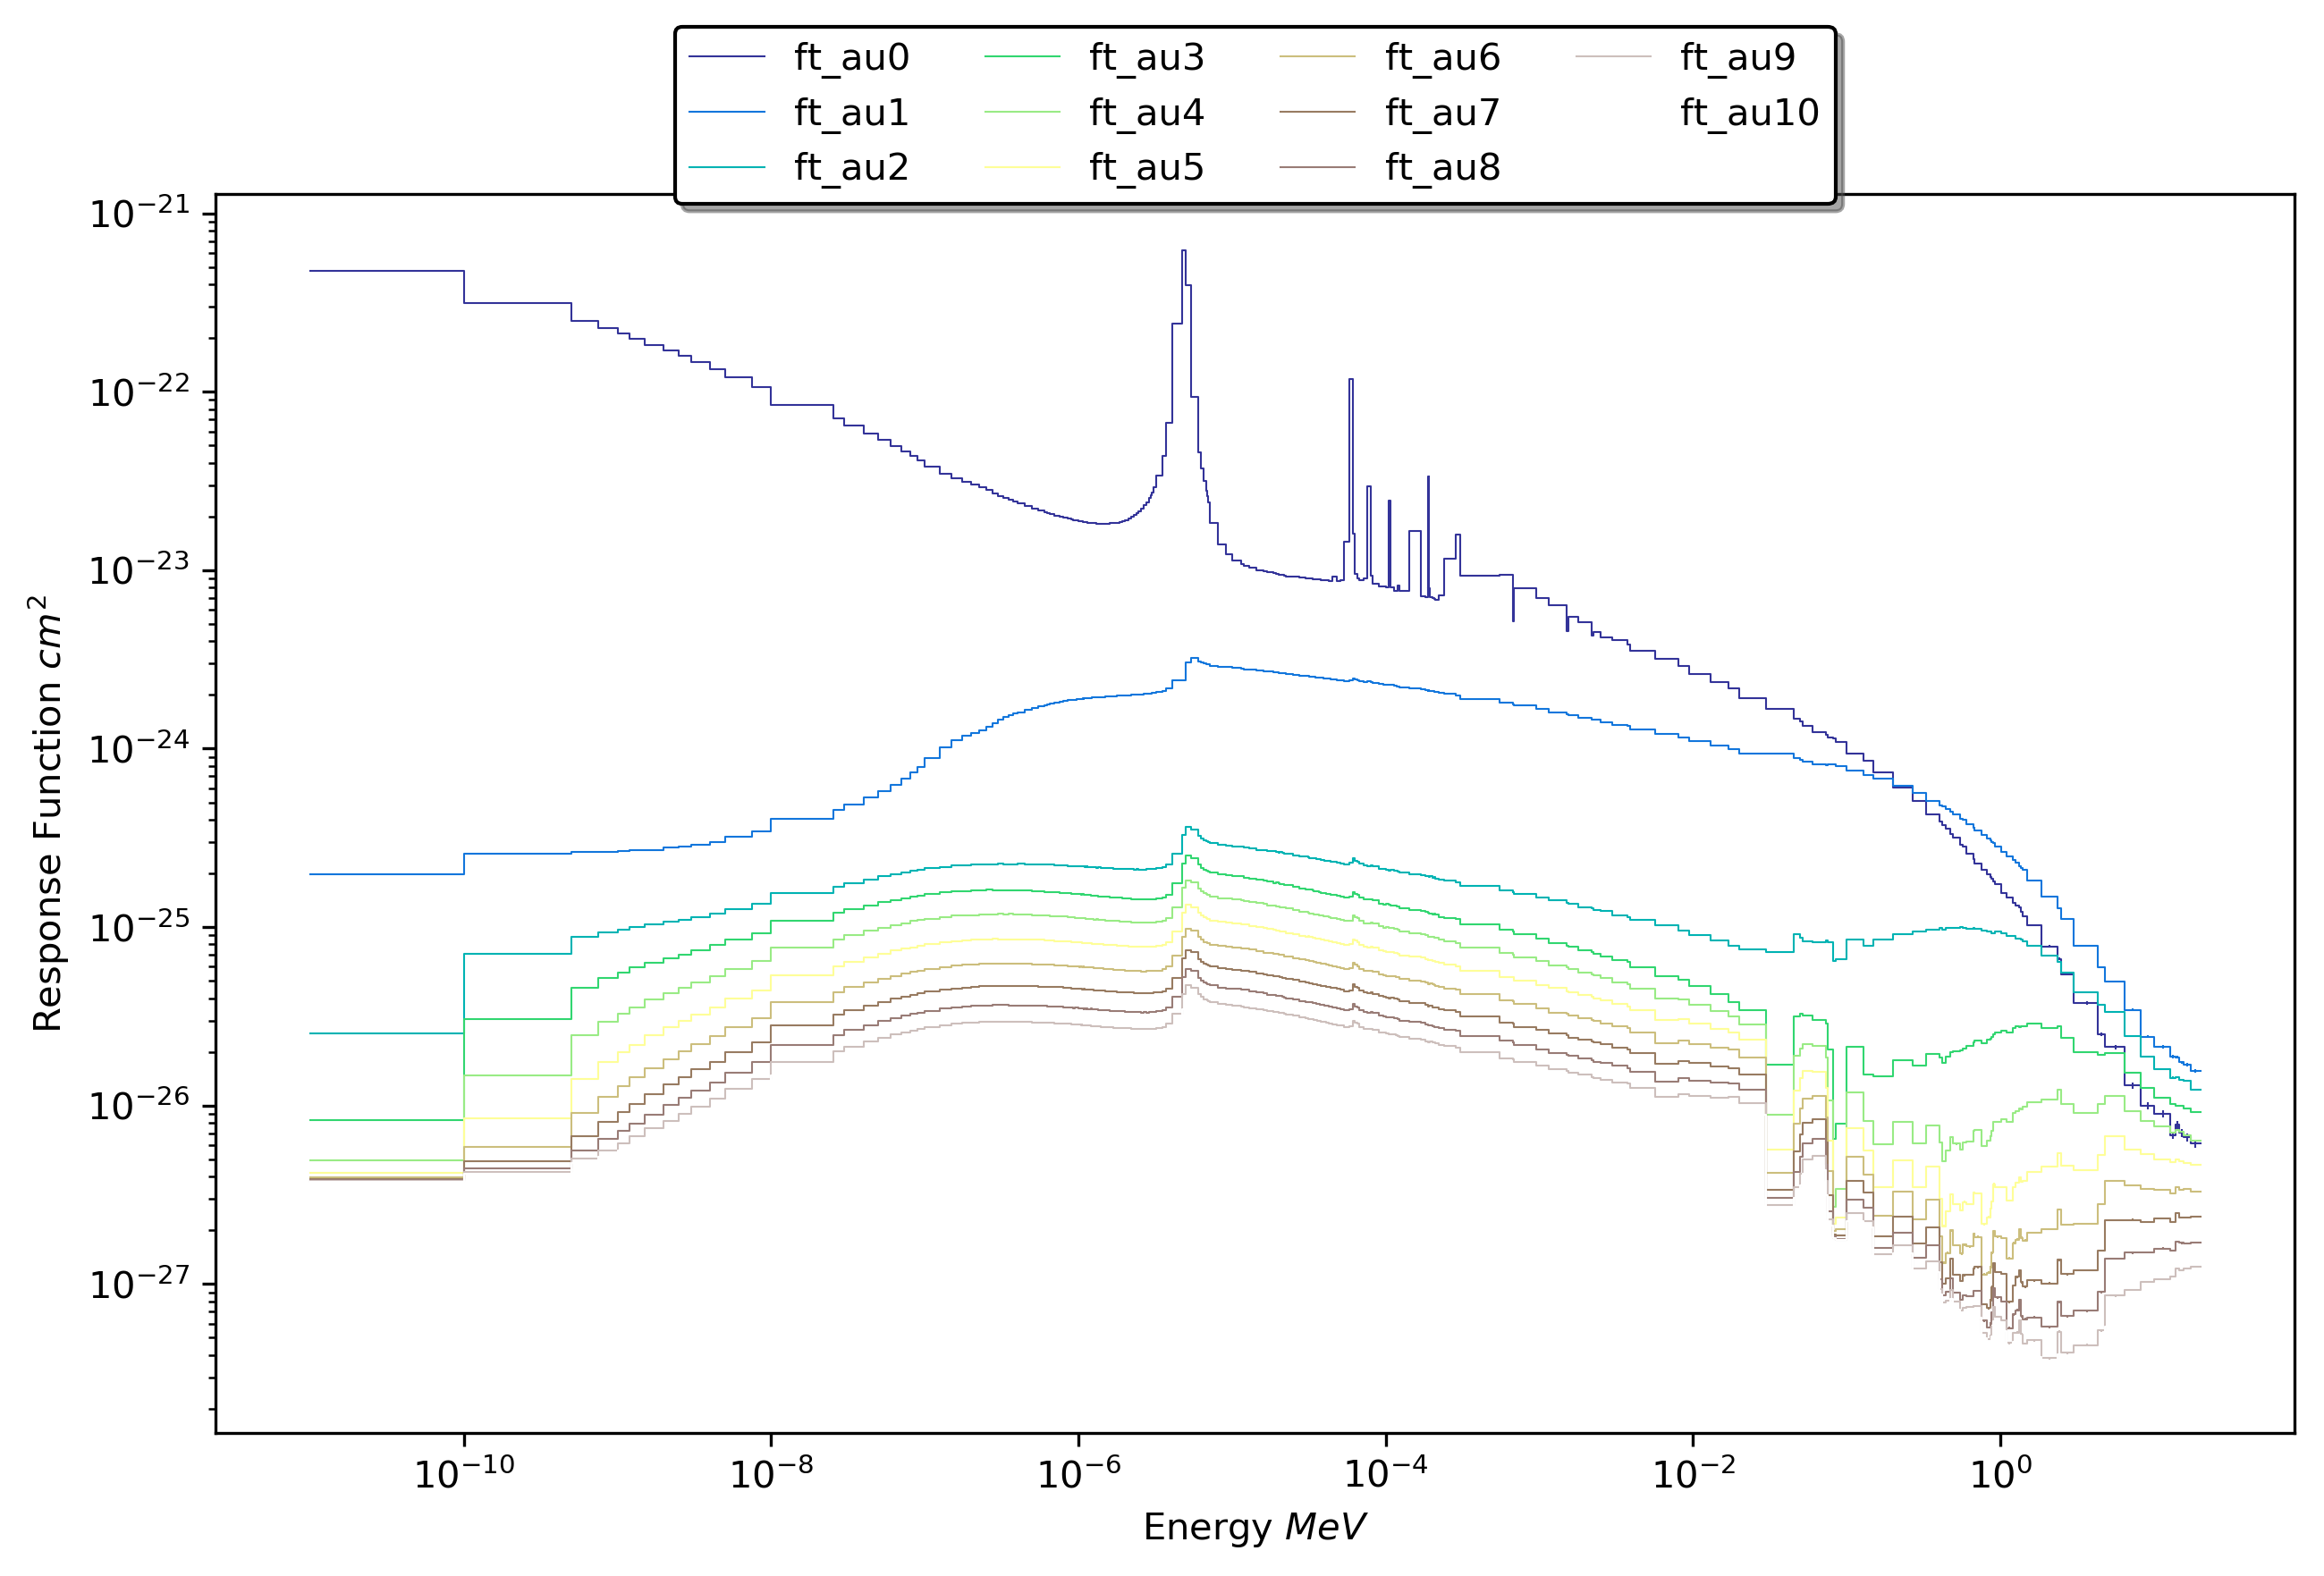
\includegraphics[height=4in]{tex/figures/ft_au.png}
\caption[Gold Foil Tube Response Functions]{The response functions for the gold foil tube.}
\label{fig:ft_au_rfs}
\end{figure}

% discuss the ft_au response functions
The response functions for the gold foil tube are pictured in \FIG{fig:ft_au_rfs}.
As distance from the tube front increases, many interesting features form and decay.
The first response very closely resembles the $^{198}$Au(n,$\gamma$) reaction, since it is exposed to the source and backscattering contributes relatively little to this response.
However, the addition of HDPE tapers the thermal tail of this response very quickly and shifts peak behavior towards the right.
The four sections that follow the first actually have an even higher response than the exposed foil.
Throughout the epithermal region, the relatively slow curvature doesn't seem much affected by the increasing foil distance, but in the fast region, a peak forms after 2", and then grows (relatively) and is pushed to the right as foil distance increases.
Overall, the goal of producing response functions that are independent was met to at least some degree with this device design.

% the bonner sphere response functions
\begin{figure}[htb]
\centering
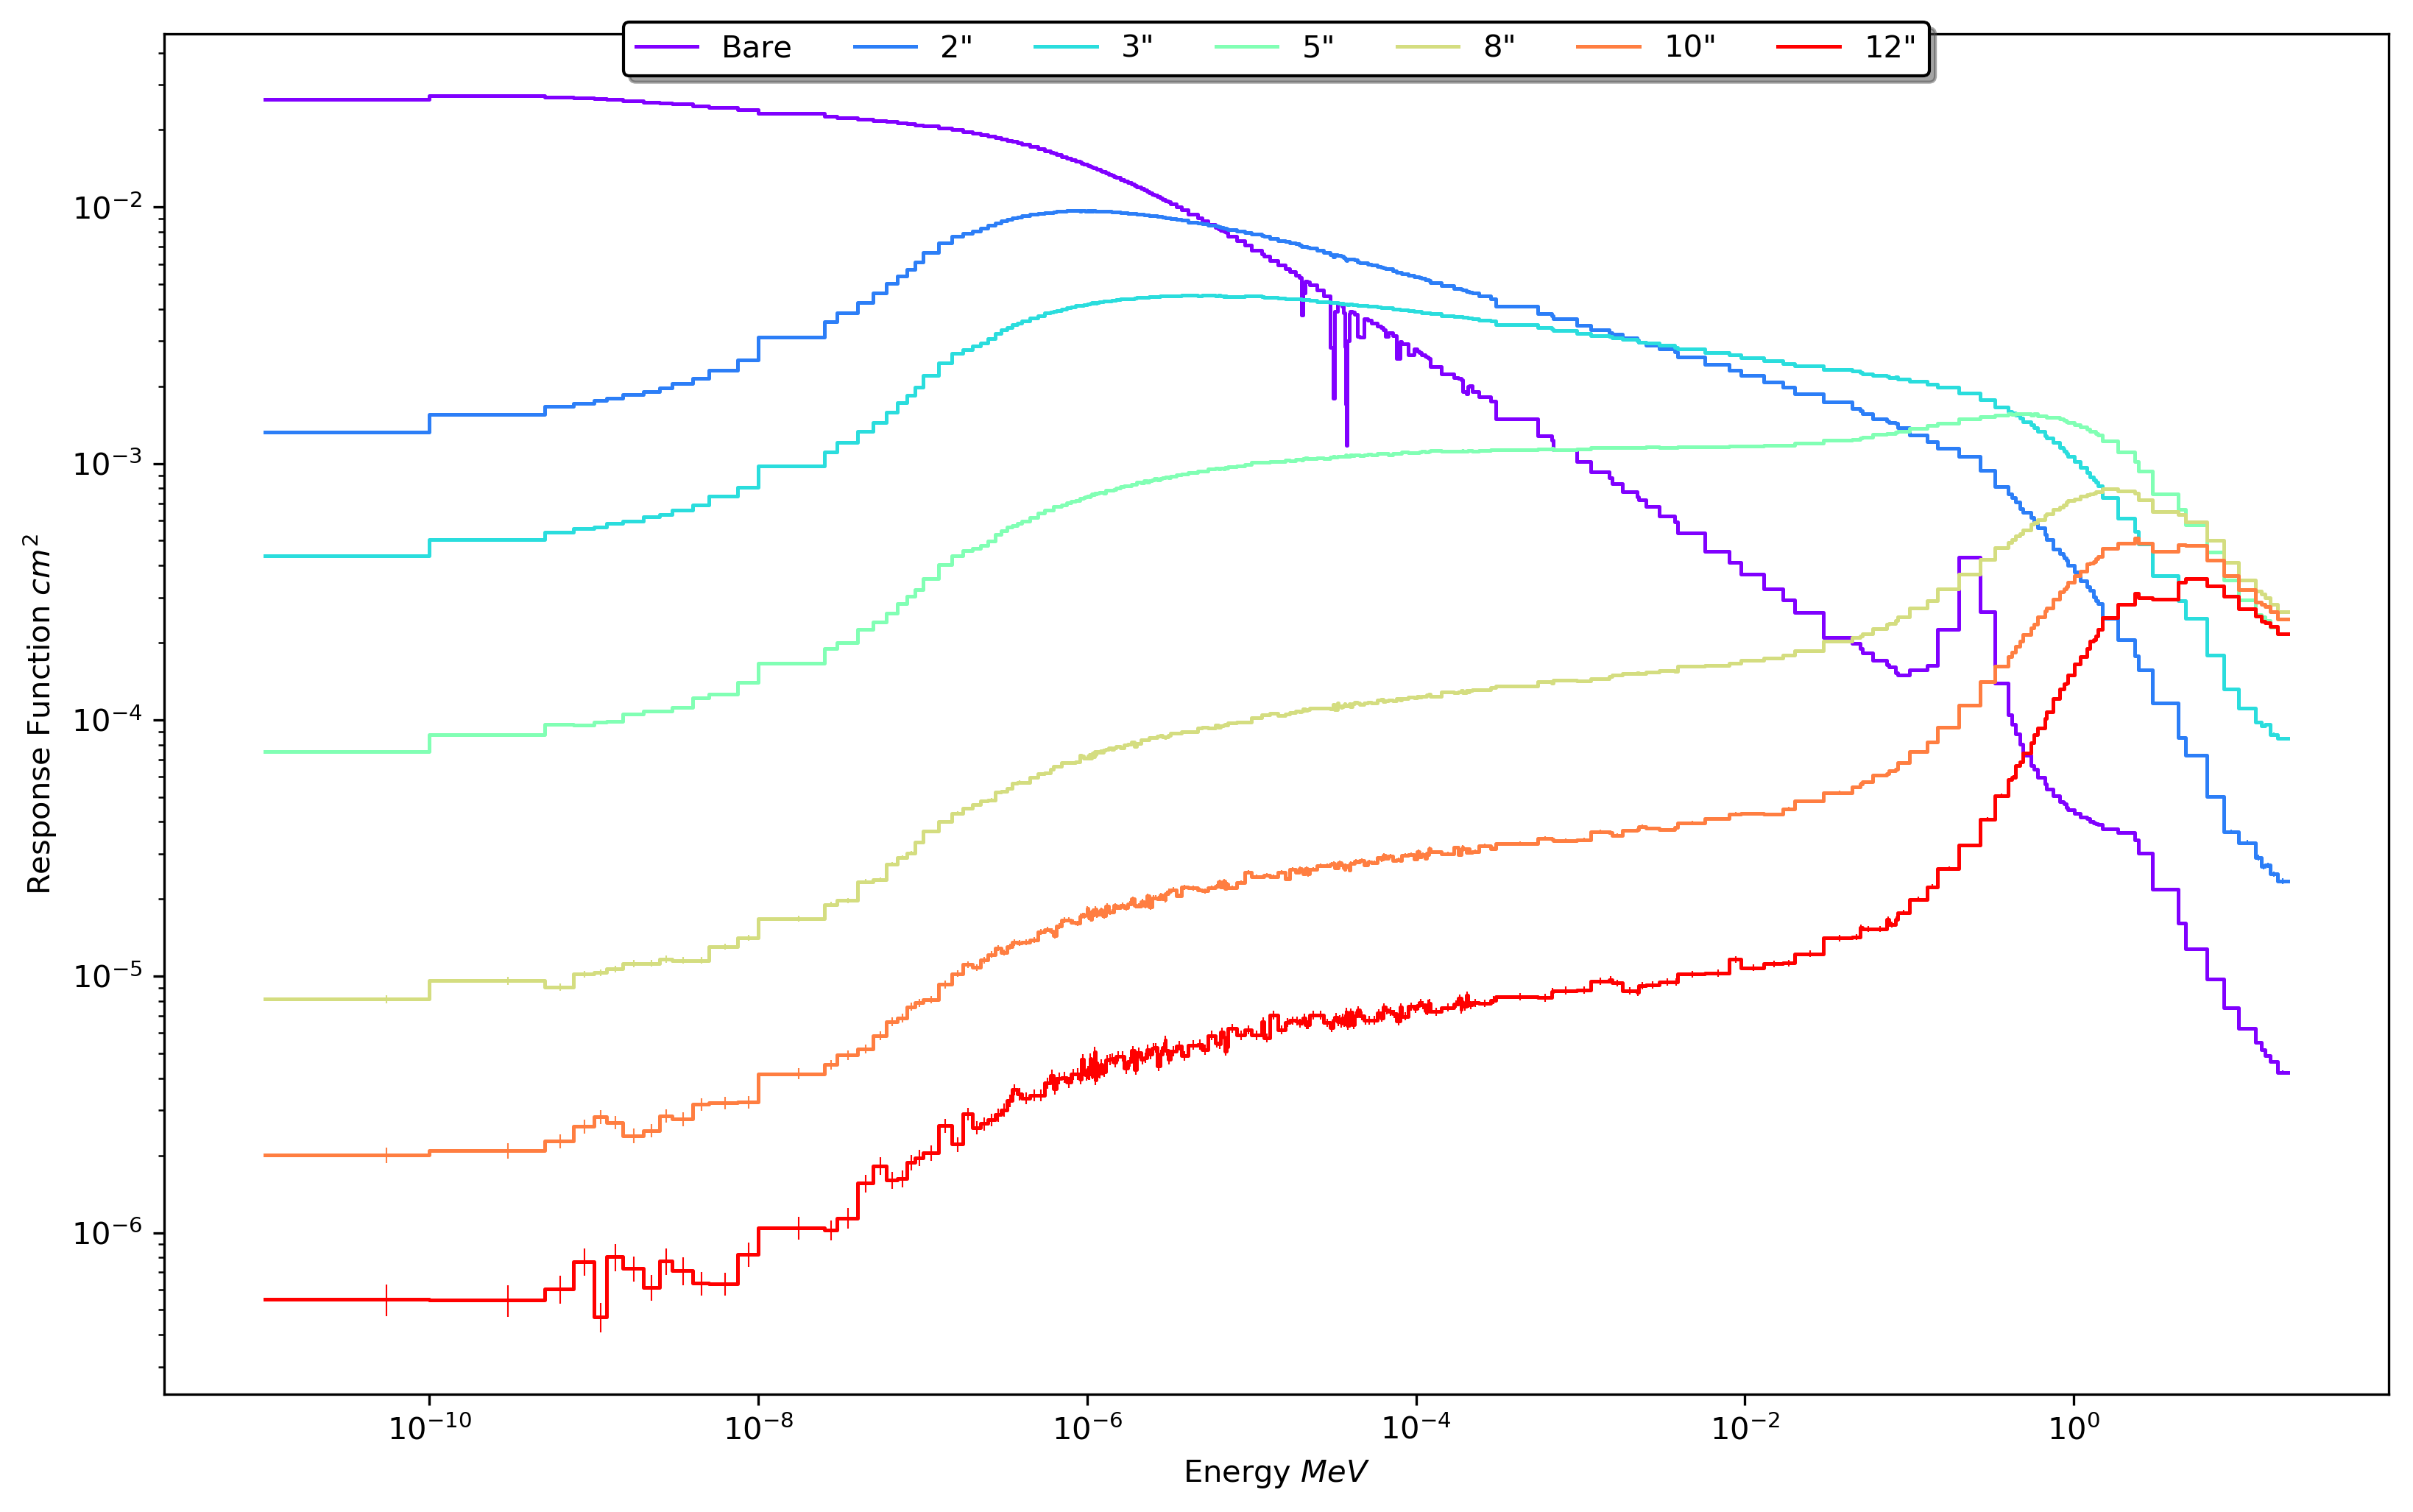
\includegraphics[height=4in]{tex/figures/bs.png}
\caption[Bonner Sphere Spectrometer Response Functions]{The response functions for the Bonner Sphere Spectrometer.}
\label{fig:bs_rfs}
\end{figure}

The trends in the BSS are similar to that of the gold foil tubes.
The bare response is thermally dominated, but as HDPE spheres are added, a peak begins to form and then is pushed towards the right.
The main difference between the two devices, besides number of detectors, is their respective responses to thermal neutrons.
Even though the thermal response is depressed in the gold foil tube, the BSS is almost completely insensitive to thermal neutrons, and there is a much larger difference between the fast and thermal response.
This is likely due to the spherical geometry used.
The BSS have lots of room around the detector for neutrons to thermalize, meaning that the fast peaks will grow to be very sharp.
In the foil tube's case, a scattered neutron is much more likely to escape the device and not be absorbed by the foil, meaning that the contribution to the fast portion of the spectrum will be much lower, relatively.

% -------------------------------------------------------------------------------------------
\section{Experimental Procedures}


\subsection{Gold Foil Tube}

% foils were individually weighed and included in table
First, the foils were individually weighted and those values are shown in \TAB{tab:au_masses}.
% the device was assembled
The device was then assembled as described in the modeling section.
% outer shielding was removed from the beam port configuration
Some of the outer shielding around the beam port was removed to access the collimator.
% the devices was attempted to fit into the beam port but deformation prevented insertion
Initially, an attempt was made to insert the device into the collimator, but deformation in the aluminum portion of the collimator prevented insertion.
% the device was ground down to fit in and inserted to where the first piece was in line with the aperture of the collimator
The first few inches of the device were then ground down with a belt sander to reduce the diameter of the device slightly.
The device was then inserted into the reactor.
% then, the reactor was powered on to __ kwth
Reactor power was brought to 100kW(th).
% the reactor remained at power for __ hours
The reactor remained at power for approximately 2.5 hours.
% then the reactor was shut down
Following the irradiation, the reactor was shut down.
% after allowing the device to cool for a bit, the individual foils were removed and bagged
A cooling period was necessary for the short-lived isotopes produced in the collimator and device to decay.
Then, the device was removed, and from the device, the individual foils were removed and bagged.
% foils were moved to an individual counting station where they were counted (gamma spec)
The foils were moved to an individual counting station, where they were sequentially counted using an HPGE.

% foil tube experimental configuration
\begin{figure}[htb]
\centering
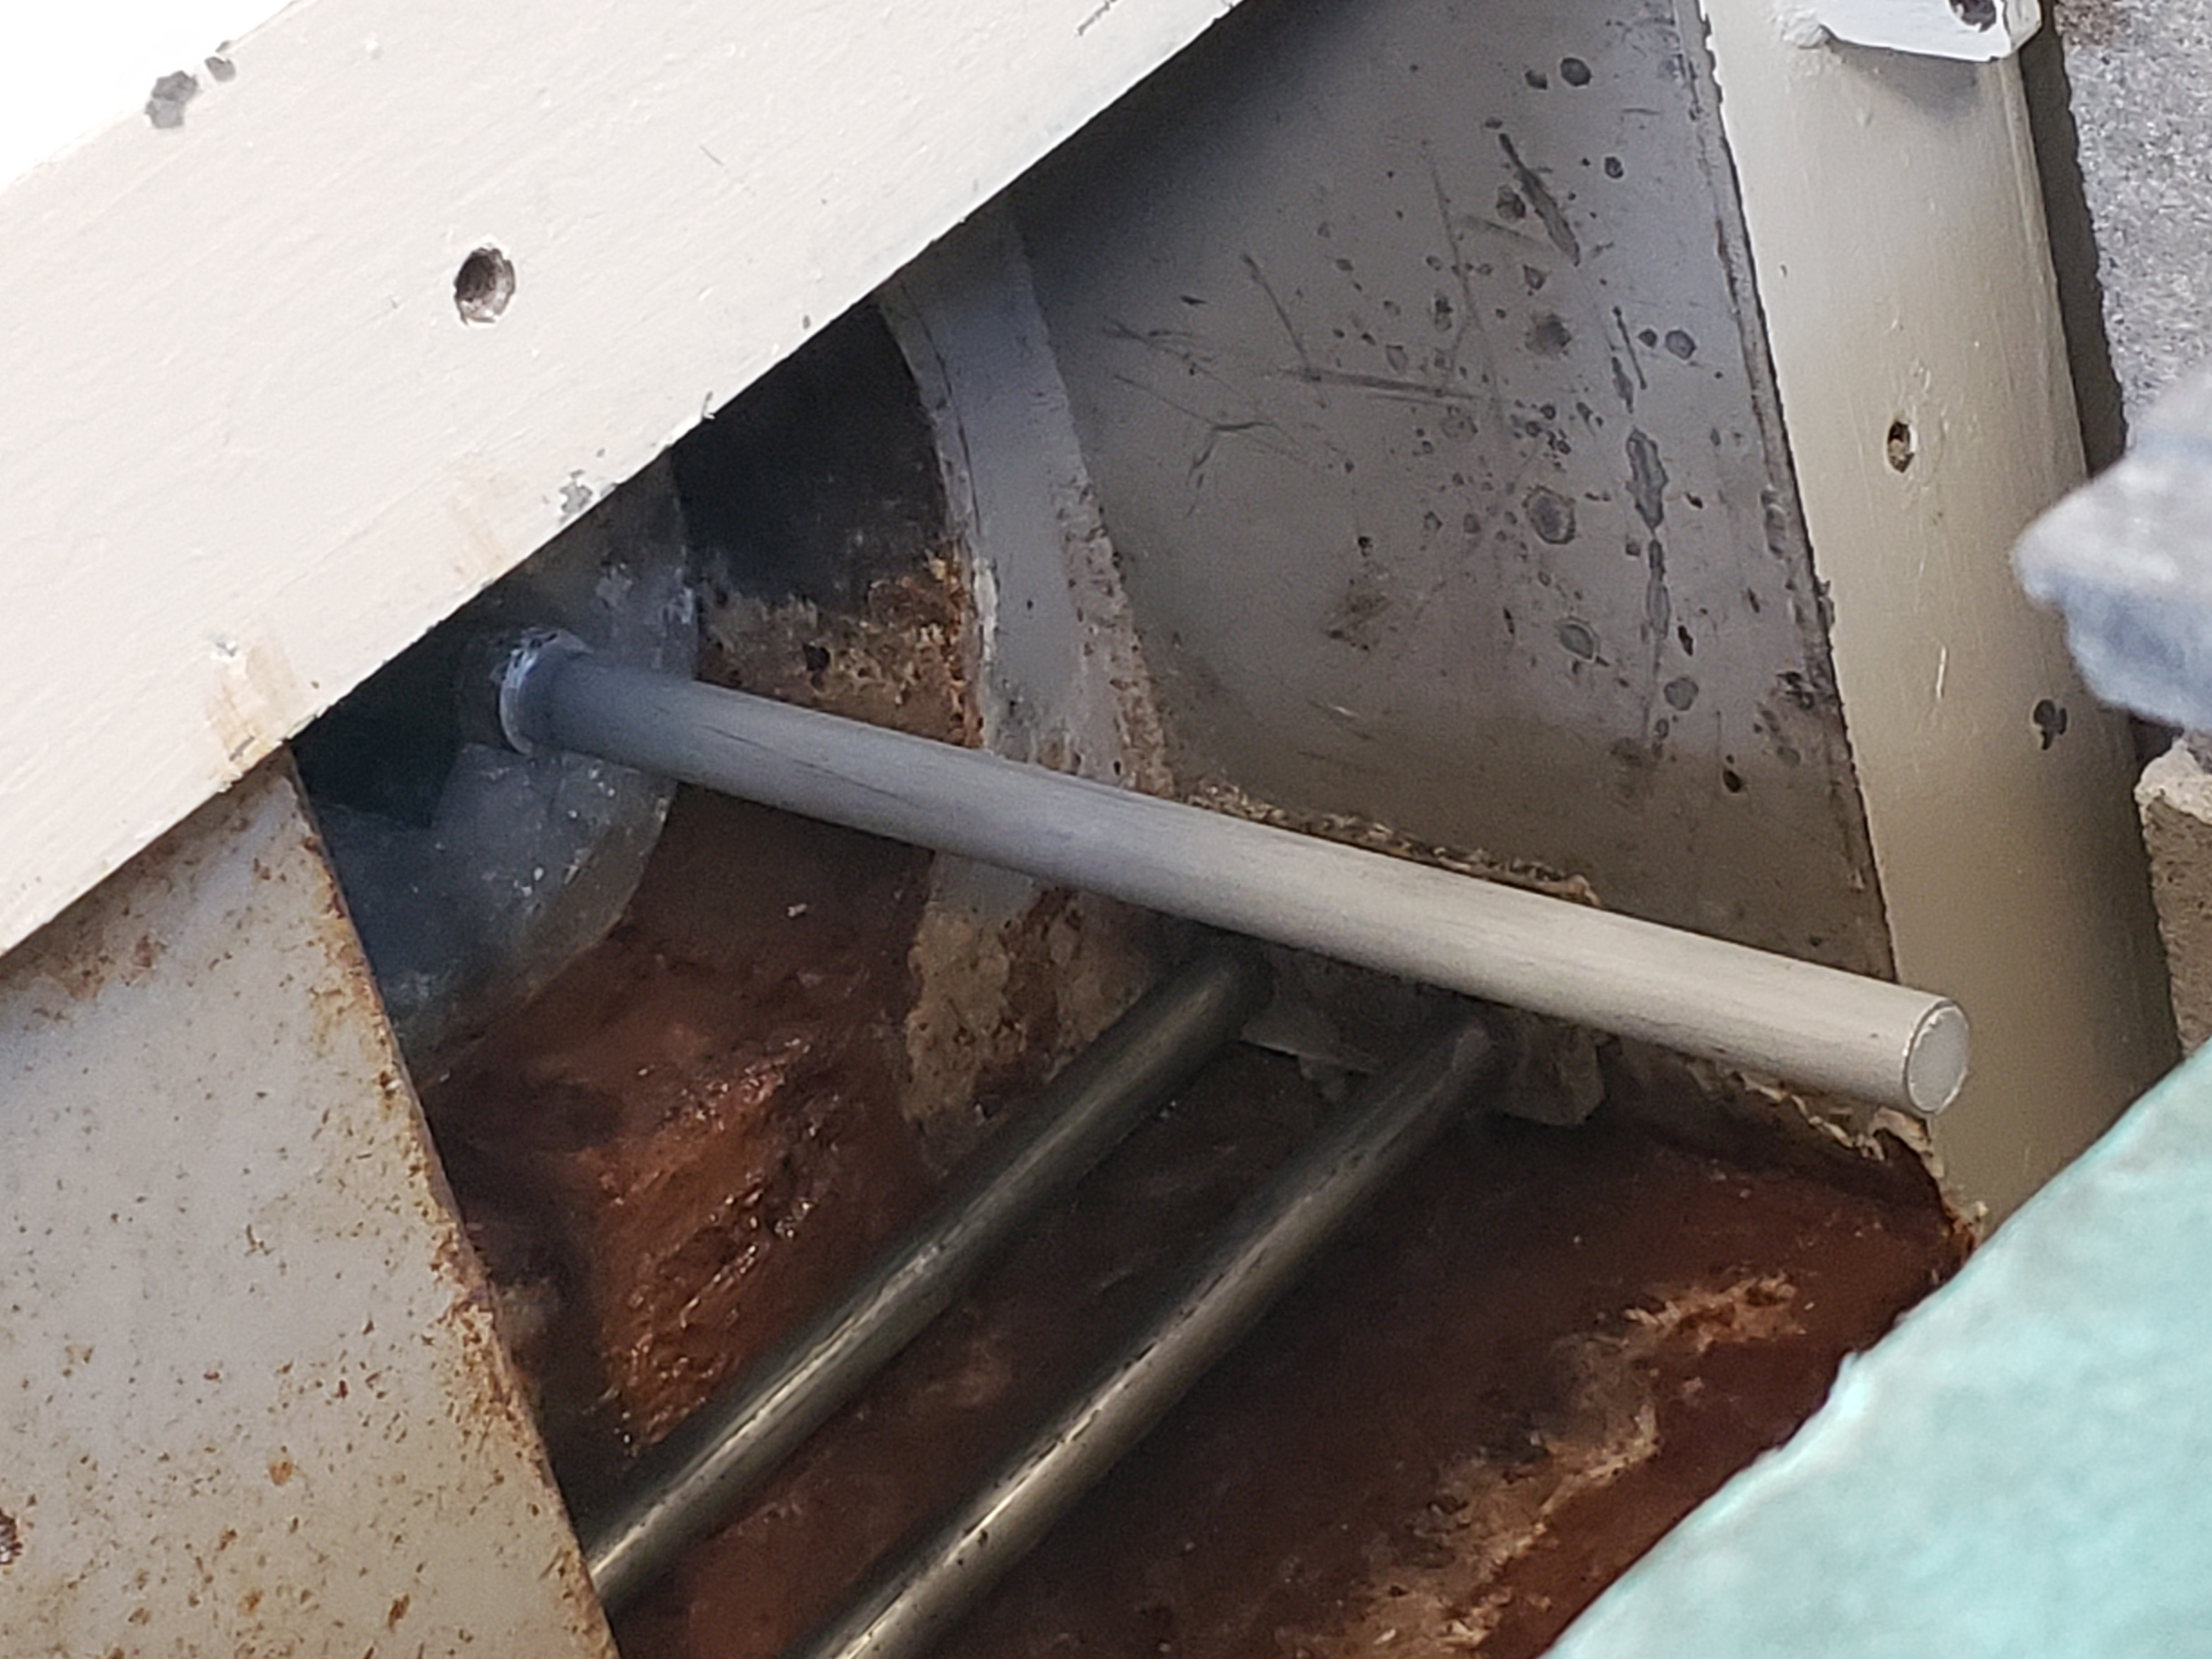
\includegraphics[height=3in]{tex/figures/ft_au_in_beam.jpg}
\caption[Gold Foil Tube Experiment]{A view of the gold foil tube inserted into the NEBP collimator.}
\label{fig:ft_au_in_beam}
\end{figure}

% this contains all of the advantg parameters
\begin{table}[h]\centering
\label{tab:au_masses}
\caption{The masses of the gold foils.}
\begin{tabular}{ r | r | l }
\toprule
Foil ID  & Position (in.)     &   Foil Mass (g)\\
2 & 0 & 0.0320\\
13 & 1 & 0.0312\\
4 & 2 & 0.0320\\
5 & 3 & 0.0318\\
6 & 4 & 0.0319\\
7 & 5 & 0.0325\\
8 & 6 & 0.0326\\
9 & 7 & 0.0320\\
10 & 8 & 0.0318\\
11 & 9 & 0.0326\\
12 & 10 & 0.0317\\
\end{tabular}
\end{table}

\subsection{Bonner Sphere Spectrometer}

% for the bonner spheres, the device was placed vertically in a manner that aligned the detection crystal with the beam at a distance of ___ cm
For the BSS irradiation, the device was positioned vertically in a manner that aligned the detection crystal with the center of the beam at a distance of (???) cm.
% the detector was set to aquire for __ s, and then the reactor was brought to __ kwth.
The detector was set to aquire for 300 s live time and then the reactor was brought to 100kW(th).
% the lld setting was adjusted to where the noise could be removed, but the lithium,T peak wasn't affected
The lld setting was electronically adjusted to reduce the detector dead time, without removing the $^6$Li(n,t) peak.
% spectra were aquired for each configuration
Spectra were aquired for the bare, 2", 3", 5", 8", 10", and 12" configurations.
For the 12" sphere, a live time of 600 seconds was used to help achieve lower counting statistics.
% the reactor was then powered off
Following the experiment, the reactor was powered off.

% ------------
% i need to put all the detection settings and stuff here
% ------------


% ------------
% also, add pictures of both setups
% ------------


% -------------------------------------------------------------------------------------------
\section{Postprocessing and Results}


\subsection{Gold Foil Tube}


% postprocessing includes taking the measured activities and converting them to saturation activities
The postprocessing necessary for a foil activation experiment involves taking the measured activities, which are reported from the gamma spectrometry software, and backing out the saturation activities for each foil.
% this is done using the following equation
This is done using the following equation,

% how to get saturation activities
\begin{equation}
\label{eqn:a_sat}
A_{sat} = A_{meas} \frac{R_{meas}}{R_{sat} n_a K I_{rel}} ,
\end{equation}

% where, (explain these terms)
where $R_{meas}$ is the ratio that corrects for decay during measurement, $R_{sat}$ is the saturation ratio which will be explained below, $n_a$ is the number of sample atoms, equal to $\rho N_A / M$, $K$ is the isotopic abundance, and $I_{rel}$ is the relative intensity of the counted gamma ray.

% give the term and explain for r_meas
The term, $R_{meas}$ is the ratio of the activity at the beginning of the gamma counting to the activity assuming the decay is constant during counting.
It is given by the following equation

% measurement ratio/correction factor
\begin{equation}
\label{eqn:r_meas}
R_{meas} = \frac{\lambda t_{meas}}{1 - e^{\lambda t_{meas}}},
\end{equation}

in which $\lambda$ is the decay constant and $t_{meas}$ is the time during measurement.

% explain the concept of saturation ratio
The saturation ratio, $R_{sat}$, is the ratio between the activity at the time of measurement and the saturation activity.
Although this value generally assumes constant production during irradiation followed by a period of decay with no production, a method has been developed that captures transient behavior in reactor fluxes which will be detailed here.

The production and decay of radioisotopes is expressed mathematically through the bateman equation,

\begin{equation}
\label{eqn:bateman}
\frac{dN(t)}{dt} = C(t) - \lambda N(t)
\end{equation}

where $N(t)$ is the number of radioactive nuclei in the sample, C(t) is the production term in nuclei per second, and $\lambda$ is the decay constant for the isotope in consideration.
The change in radionuclei is simply the production minus the loss.
The relationship between activity and radionuclides, $A(t) = \lambda N(t)$ allows us to convert \EQ{eqn:bateman} into the following,

\begin{equation}
\label{eqn:bateman_activity}
\frac{A(t)}{dt} = \lambda (C(t) - A(t)).
\end{equation}

We can then divide each of the terms by $C_{sat}$ which is the isotopic production at nominal power.
This value is equal to the saturation activity, since the activity at $t = \inf$ for nominal power is equal to the production at that power.

\begin{equation}
\label{eqn:bateman_ratios}
\frac{A(t) / C_{sat}}{dt} = \lambda (\frac{C(t)}{C_{sat}} - \frac{A(t)}{C_{sat}})
\end{equation}

Two facts allow us to simplify \EQ{eqn:bateman_ratios} into a useful form.
First, because $A_{sat} = C_{sat}$, any $A(t) / C_{sat} = A(t) / A_{sat}$, so we can replace these terms with a defined term, $R_{sat}(t)$ which is the ratio of the activity at time $t$ to the saturation activity.
Second, although we don't have access to the $C(t)$ or $C_{sat}$ terms since they require the (currently unknown) flux, we do have access to power data.
Because isotopic production is approximately proportional to reactor power, $C(t) \propto P(t)$, this means that $C(t) / C_{sat} \approx P(t) / P_{nominal}$.
We will replace this power ratio with the term $P_{f}(t)$, which is simply the time dependent ratio of the power to the nominal power.

\begin{equation}
\label{eqn:bateman_r_sat}
\frac{R_{sat}(t)}{dt} = \lambda (P_{f}(t) - R_{sat}(t))
\end{equation}

This equation can be solved to find $R_{sat}$ at the time of measurement using a numerical solver, in our case, {\tt scipy}'s {\tt odeint}.
The data for $P_{f}(t)$ is simply normalized strip chart data collected from an in-core fission chamber.


% ---------------------
% fix this table later
% ---------------------

% this contains all of the correction factors and foil activities
\begin{table}[h]\centering
\label{tab:a_sat}
\caption{The correction factors and foil activities.}
\begin{tabular}{ r | r | r | l | r }
\toprule
Position (in.)  & $A_{meas}$ (Bq) & $R_{meas}$  & $R_{sat}$   &   $A_{sat}$  (Bq)\\
0 & 1483.73 & 1.00089 & 0.02268 & 65468.28 \\
1 & 58.60 & 1.00590 & 0.02262 &  2605.89  \\
2 & 8.92 & 1.03805 & 0.02196 &   422.02  \\
3 & 4.06 & 1.06581 & 0.0204  &   212.01  \\
4 & 2.58 & 1.14023 & 0.01574  &   186.96  \\
5 & 1.60 & 1.27976 & 0.01340 &      153.12  \\
6 & 0.72 & 1.26894 & 0.00794 &       115.22  \\
7 & 0.37 & 1.27340 & 0.00483 &      97.03   \\
8 & 0.17 & 1.41587 & 0.00256 &       95.65\\
\end{tabular}
\end{table}

% foil responses
\begin{figure}[htb]
\centering
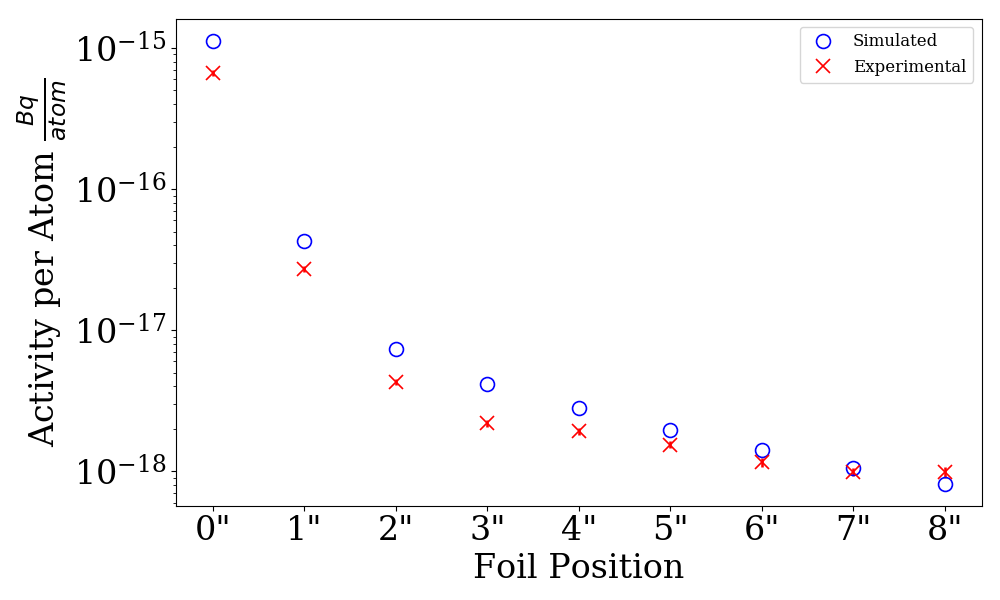
\includegraphics[height=3in]{tex/figures/compare_activities.png}
\caption[Foil Activities]{A comparison of the simulated and experimentally obtained foil activities.}
\label{fig:compare_activities}
\end{figure}


\subsection{Bonner Sphere Spectrometer}

The BSS data was processed simply by taking the area under the LiI reaction peaks and dividing that value by the live time of the detector.
These values are presented in \TAB{tab:bss}.

% bss response integration
\begin{figure}[htb]
\centering
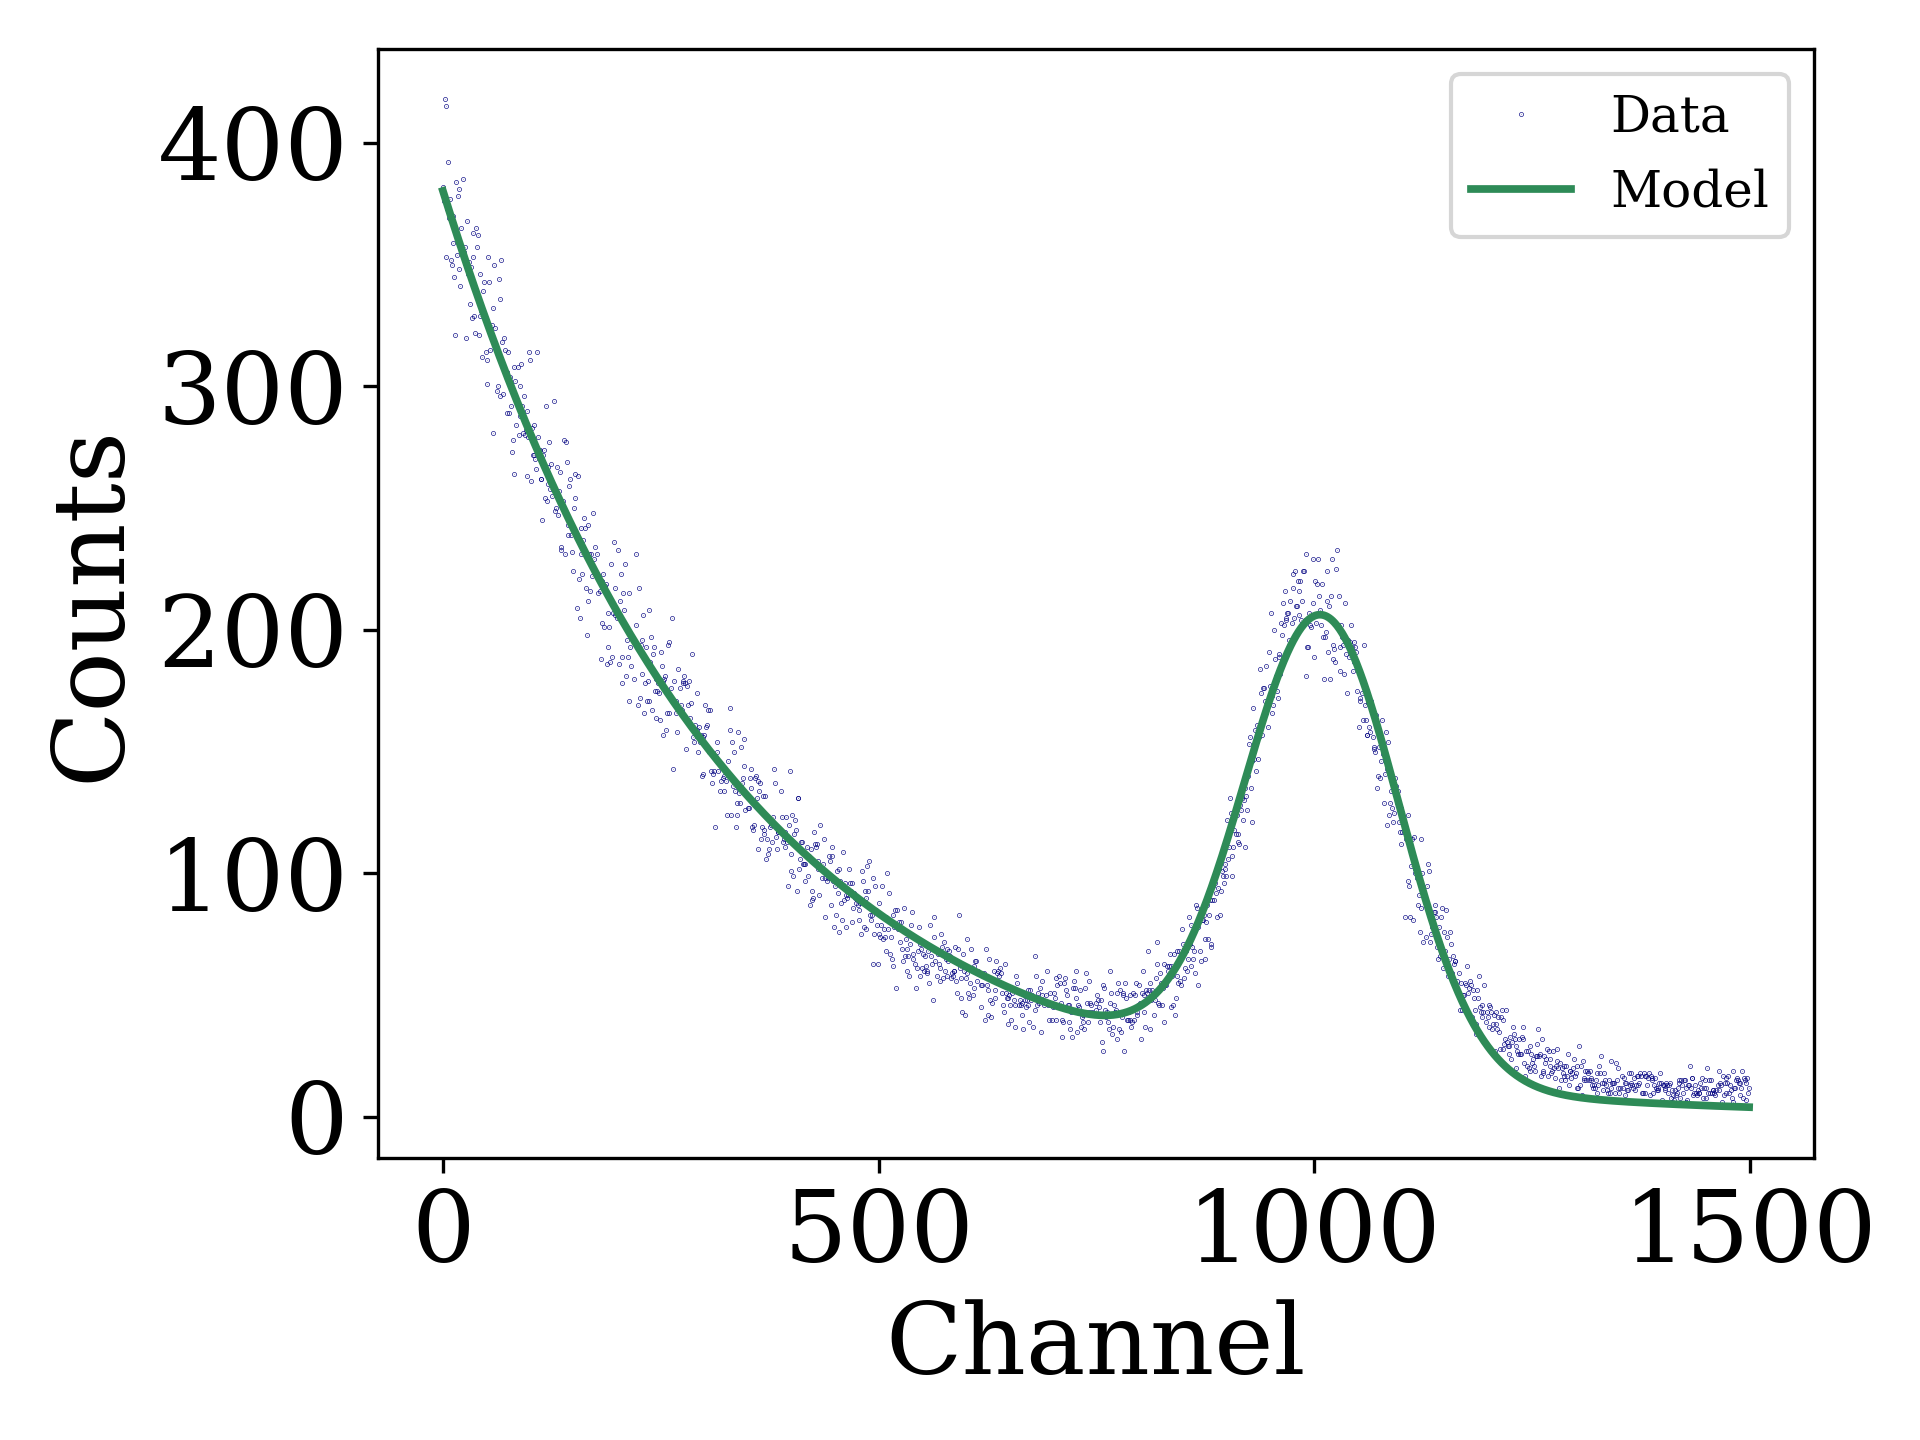
\includegraphics[height=3in]{tex/figures/bs4_spectrum.png}
\caption[8" BSS Spectrum]{The 8" sphere's gamma-ray spectrum and the model used to find the integral response.}
\label{fig:compare_countrates}
\end{figure}


% the bss count rates
\begin{table}[h]\centering
\label{tab:bss}
\caption{The BSS count rates from the experiment.}
\begin{tabular}{ r | r }
\toprule
Sphere (in.)  & Count Rate $s^{-1}$\\
Bare & 1626.76\\
2  & 1062.40\\
3 & 3891.13\\
5 & 417.24\\
8 & 139.72\\
10 & 70.75\\
12 & 37.43\\
\end{tabular}
\end{table}

% bss responses
\begin{figure}[htb]
\centering
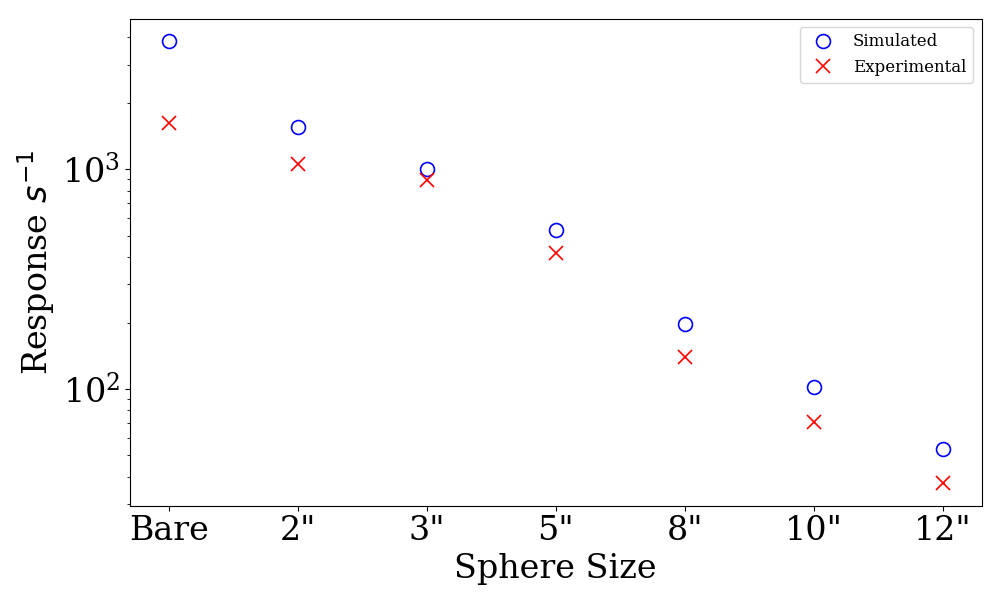
\includegraphics[height=3in]{tex/figures/compare_countrates.png}
\caption[BSS Responses]{A comparison of the simulated and experimentally obtained BSS responses.}
\label{fig:compare_countrates}
\end{figure}


% -------------------------------------------------------------------------------------------
\section{Spectral Unfolding}

\subsection{Methods and Parameters}

% the responses and response functions were used with the unfolding methods described in ch2 to obtain solution spectra
The detector responses and response functions were unfolded with the methods described in chapter two to obtain a set of solution spectra.
% the bss and ft_au results were first considered separately, then combined
The responses from the foil tube and the BSS were first considered separetely, then combined into a single vector to produce a third spectrum for each unfolding method.
% both the gravel and maxed unfolding algorithms were used with these data
The Gravel, Doroshenko, and MAXED unfolding algorithms were used.
% for gravel, 50 iterations were used
For both Gravel and Doroshenko, the termination criteria was set at 50 iterations.
% for maxed, the parameter omega was set using the number of detectors for each dataset, 9 for the foil tube, 7 for the bss, and 16 for the combined set
For MAXED, the parameter Omega was set using the number of detectors for each dataset, 9 for the foil tube, 7 for the BSS, and 16 for the combined case.
% then, the maxed portion was repeated, while first scaling the default spectrum
Then, the MAXED unfolding was repeated, but with a scaled default spectrum.
In this case, scaled means that the default spectrum was normalized so the average of the computed responses was equal to the average of the experimentally obtained responses before unfolding.

\subsection{Results and Discussion}


\begin{figure}[htb]
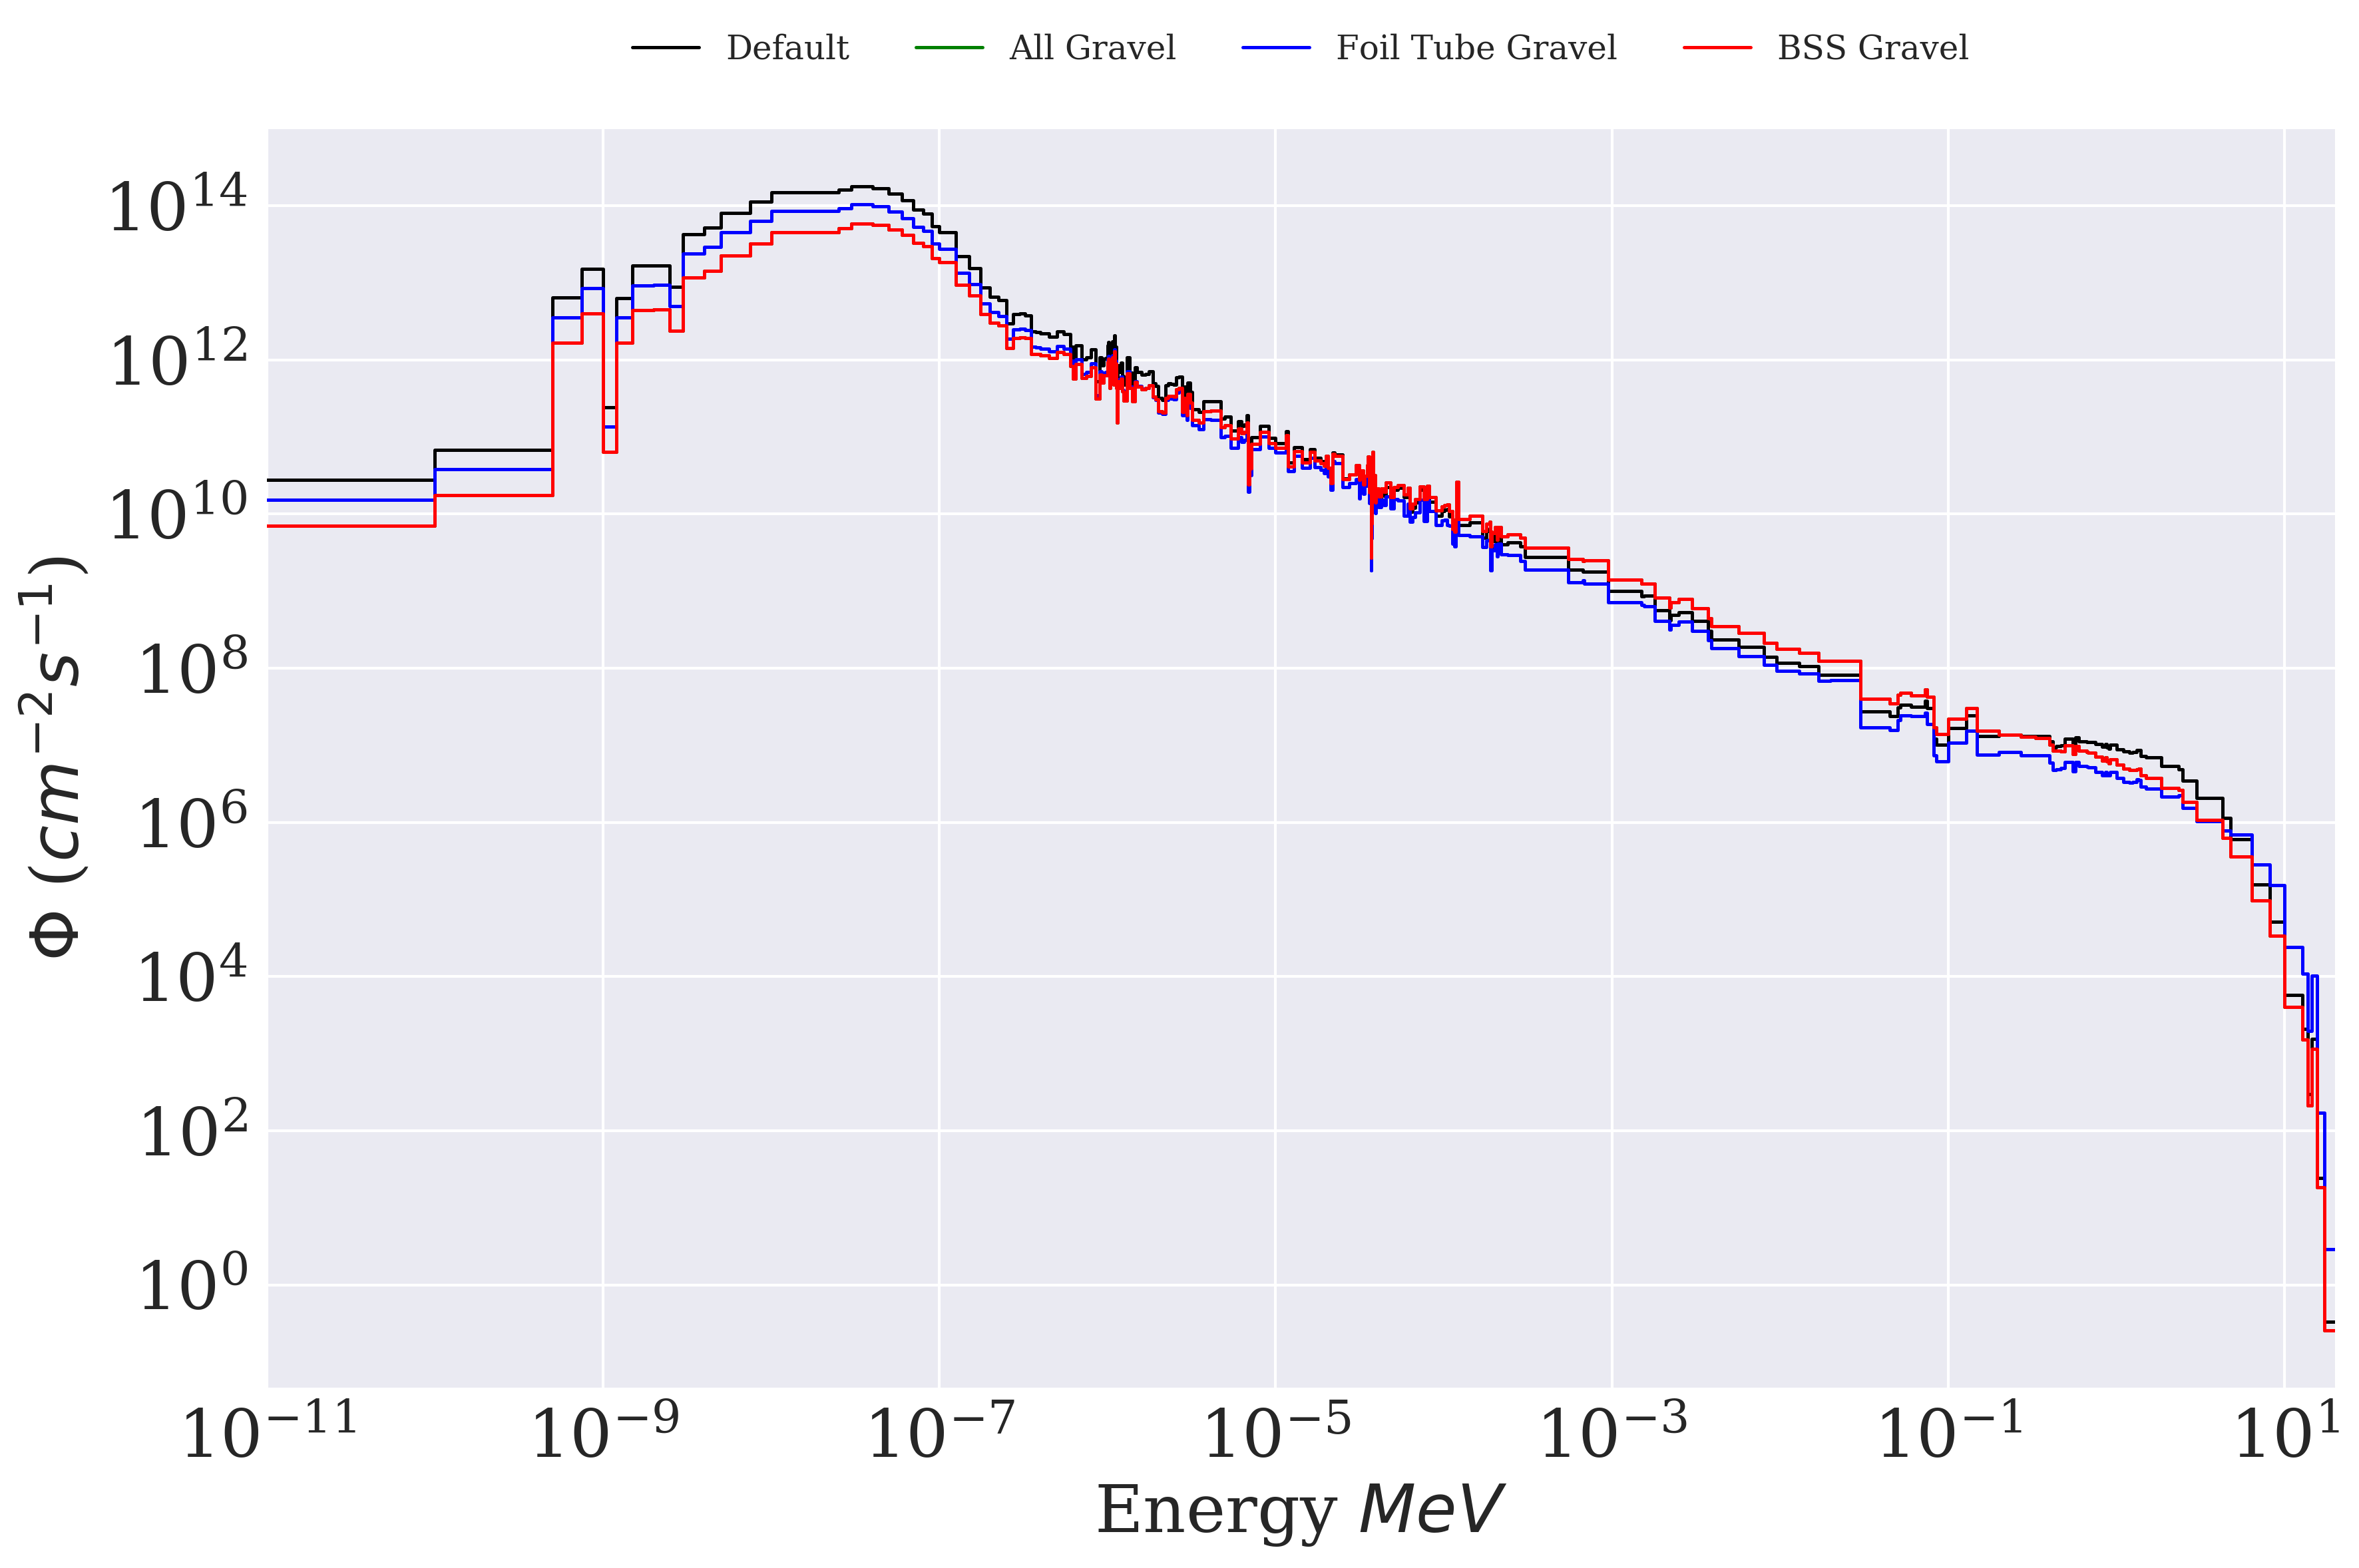
\includegraphics[height=3.8in]{tex/figures/unfolded_gr.png}
\caption[Gravel Unfolded Spectra]{The unfolded NEBP spectra obtained from using the Gravel method.}
\label{fig:unfolded_gr}
\end{figure}

% here gravel results are presented first
Here, the Gravel results are presented in \FIG{fig:unfolded_gr}
% as seen in the figure, the bss and ft_au results show good agreeance with one another
As seen in the figure, the foil tube and BSS results show good agreeace with one another.
% all of the major features from the default spectrum are preserved
All of the major features from the default spectrum are preserved.
% the ft_au results unfold to a slightly higher thermal flux than the bss where as the bss show slightly higher fast region
Some differences appear between the two datasets, where the foil tube shows a slightly higher thermal flux and the BSS is larger through a portion of the fast region.
% the combined results cannot be seen as they are covered by the ft_au
The combined results cannot be seen as they are covered by the foil tube data.
% this is because with gravel, smaller error responses are weighted heavier and the errors are much smaller for the gold foils than for the bss
This is due to the fact that the gravel algorithm will base its manipulation on relative error, meaning that smaller error (more well-known) responses will affect the final results more, and the errors from the foil tube are much smaller than the BSS results.

\begin{figure}[htb]
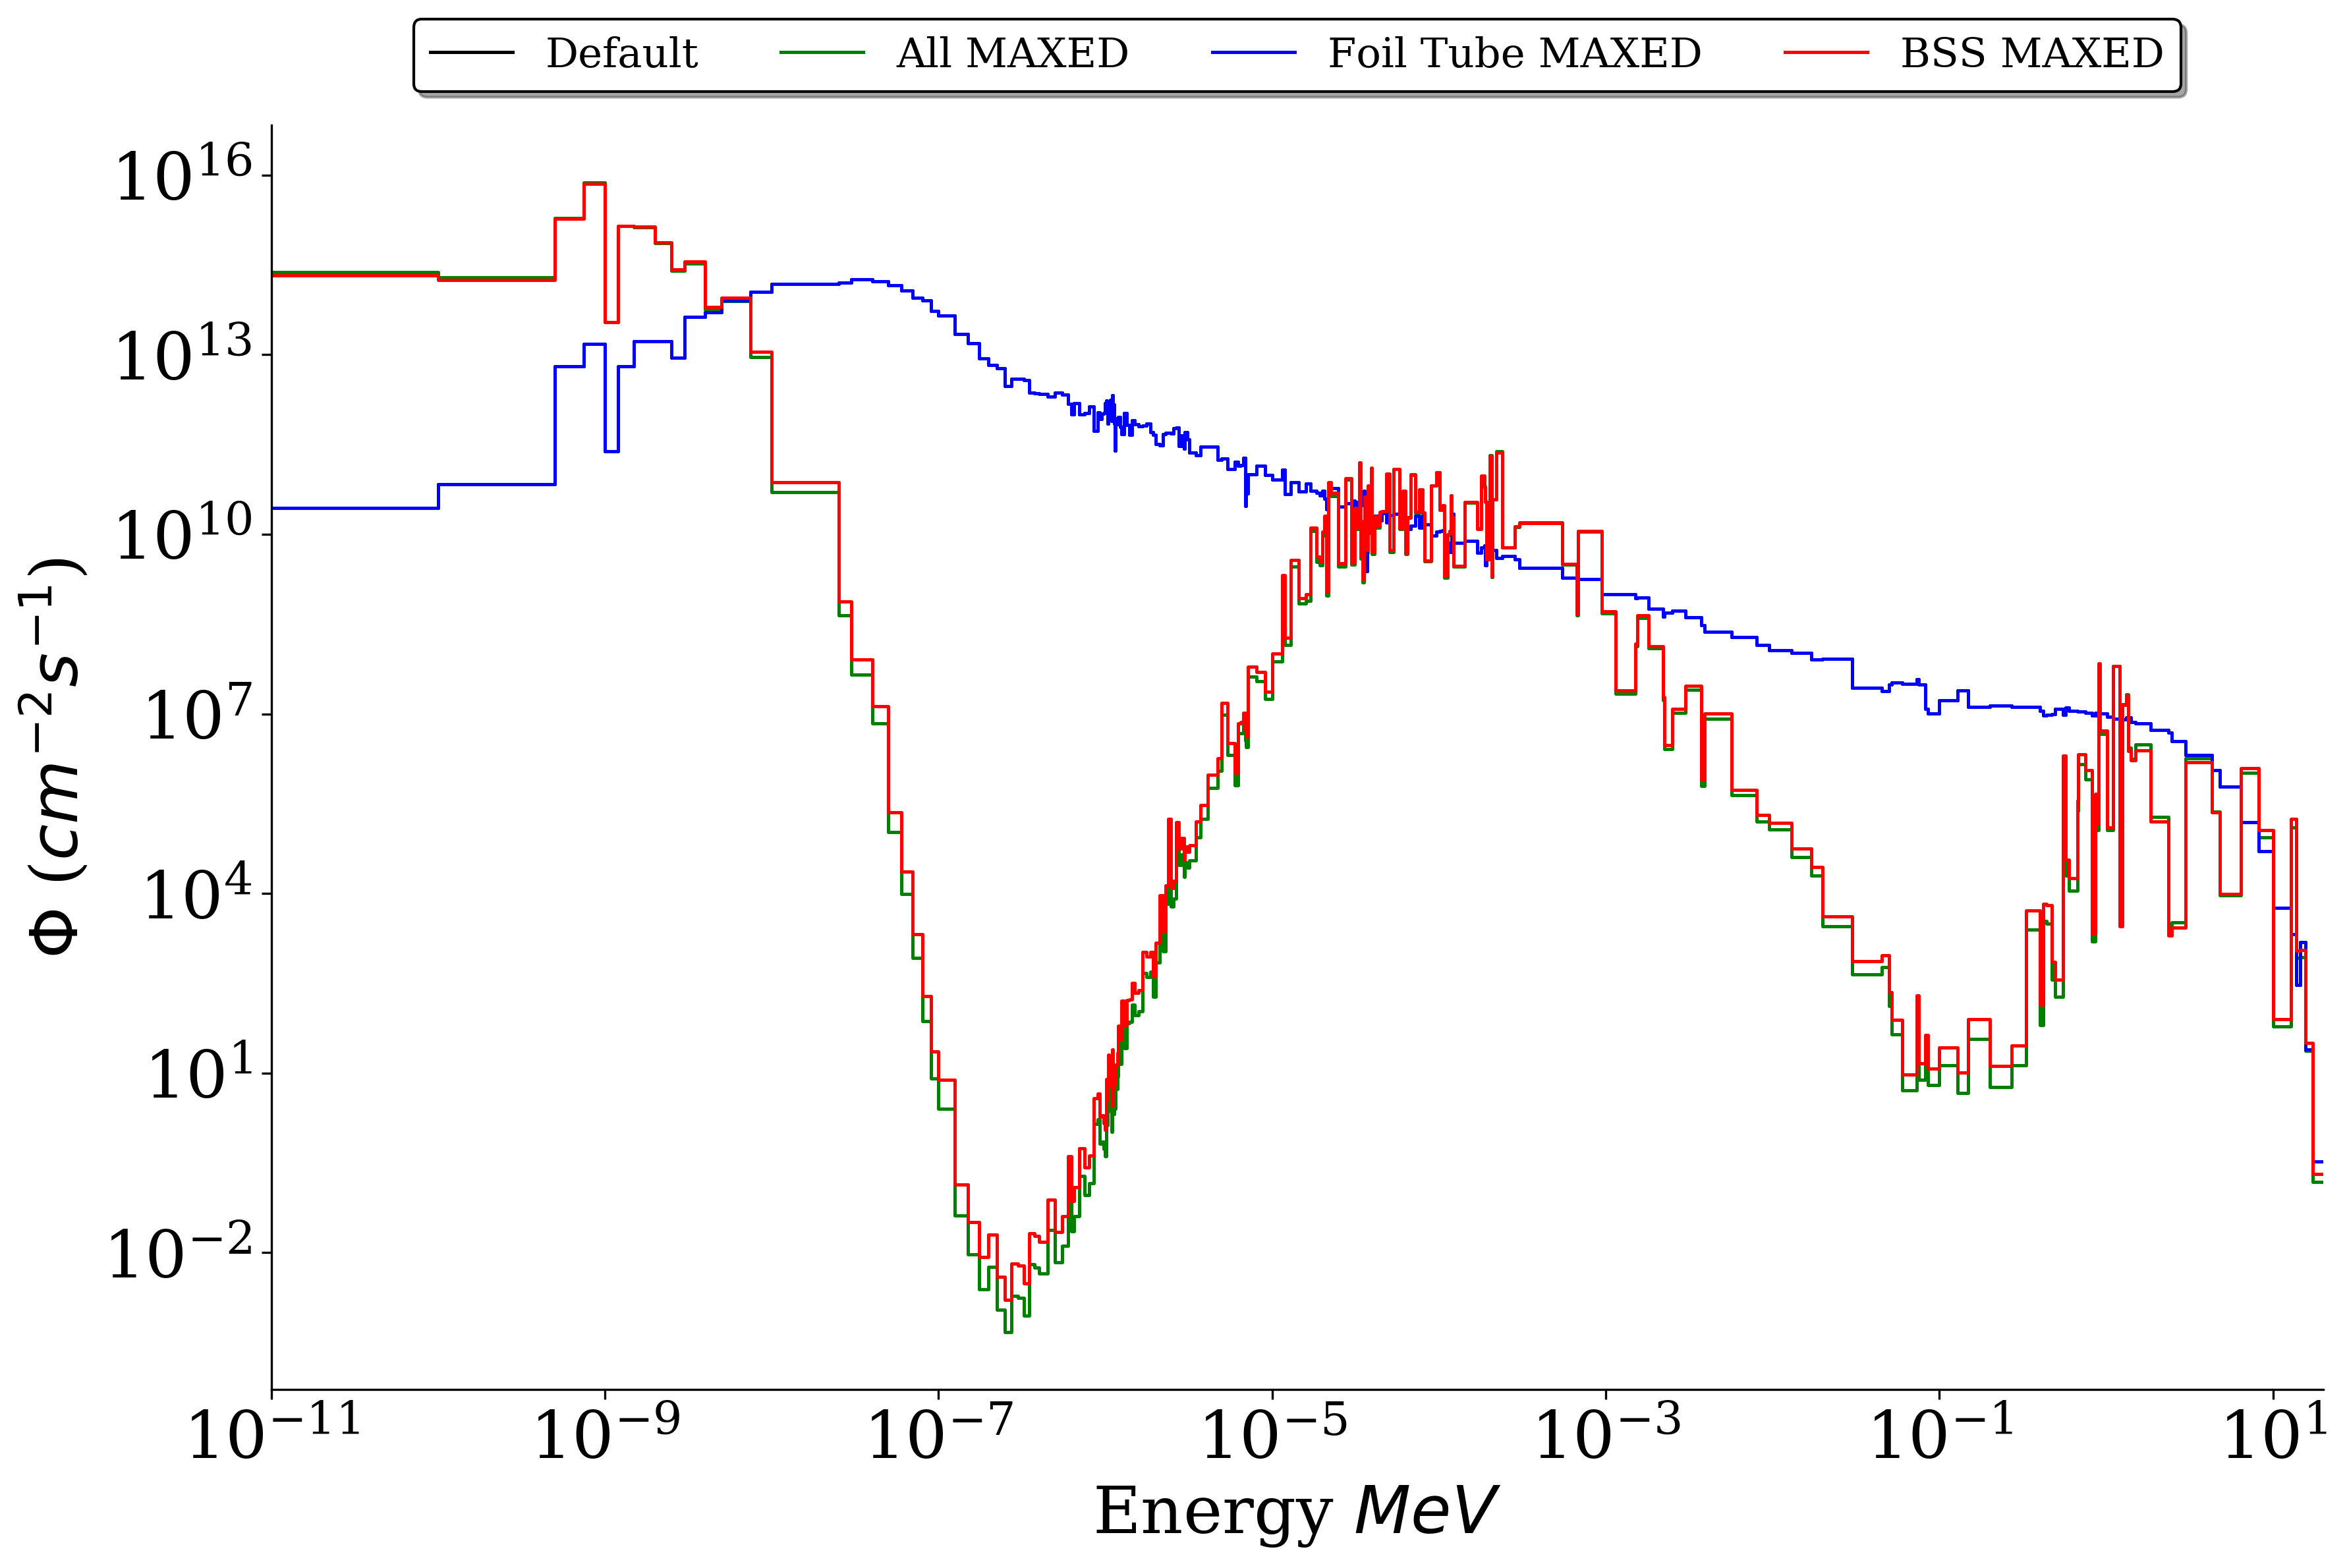
\includegraphics[height=3.8in]{tex/figures/unfolded_mx.png}
\caption[MAXED Unfolded Spectra]{The unfolded NEBP spectra obtained using the MAXED method.}
\label{fig:unfolded_mx}
\end{figure}

% these results shown in FIG are from the maxed unfolding.
Seen in \FIG{fig:unfolded_mx} are the results from the MAXED unfolding.
% in the case of the bss and combined case, the results produced are very unphysical
In the BSS and combined cases, the results produced appear very unphysical.
% this is likely due to the fact that the spectrum is trying to fit the data while staying close to the default spectrum
This is likely due to the fact that the algorithm is trying to fit the data while retaining some values close to the defaults spectrum to maximize the cross entropy between the two spectra.
% in the ft_au case, the default spectrum remains unchanged, indicating that the default spectrum actually represents a decent fit of the data
The default spectrum remains unchanged for the foil tube case, which indicates that the default spectrum actually represents a decent fit of the data, although it's still not as close as in the Gravel case.

\begin{figure}[htb]
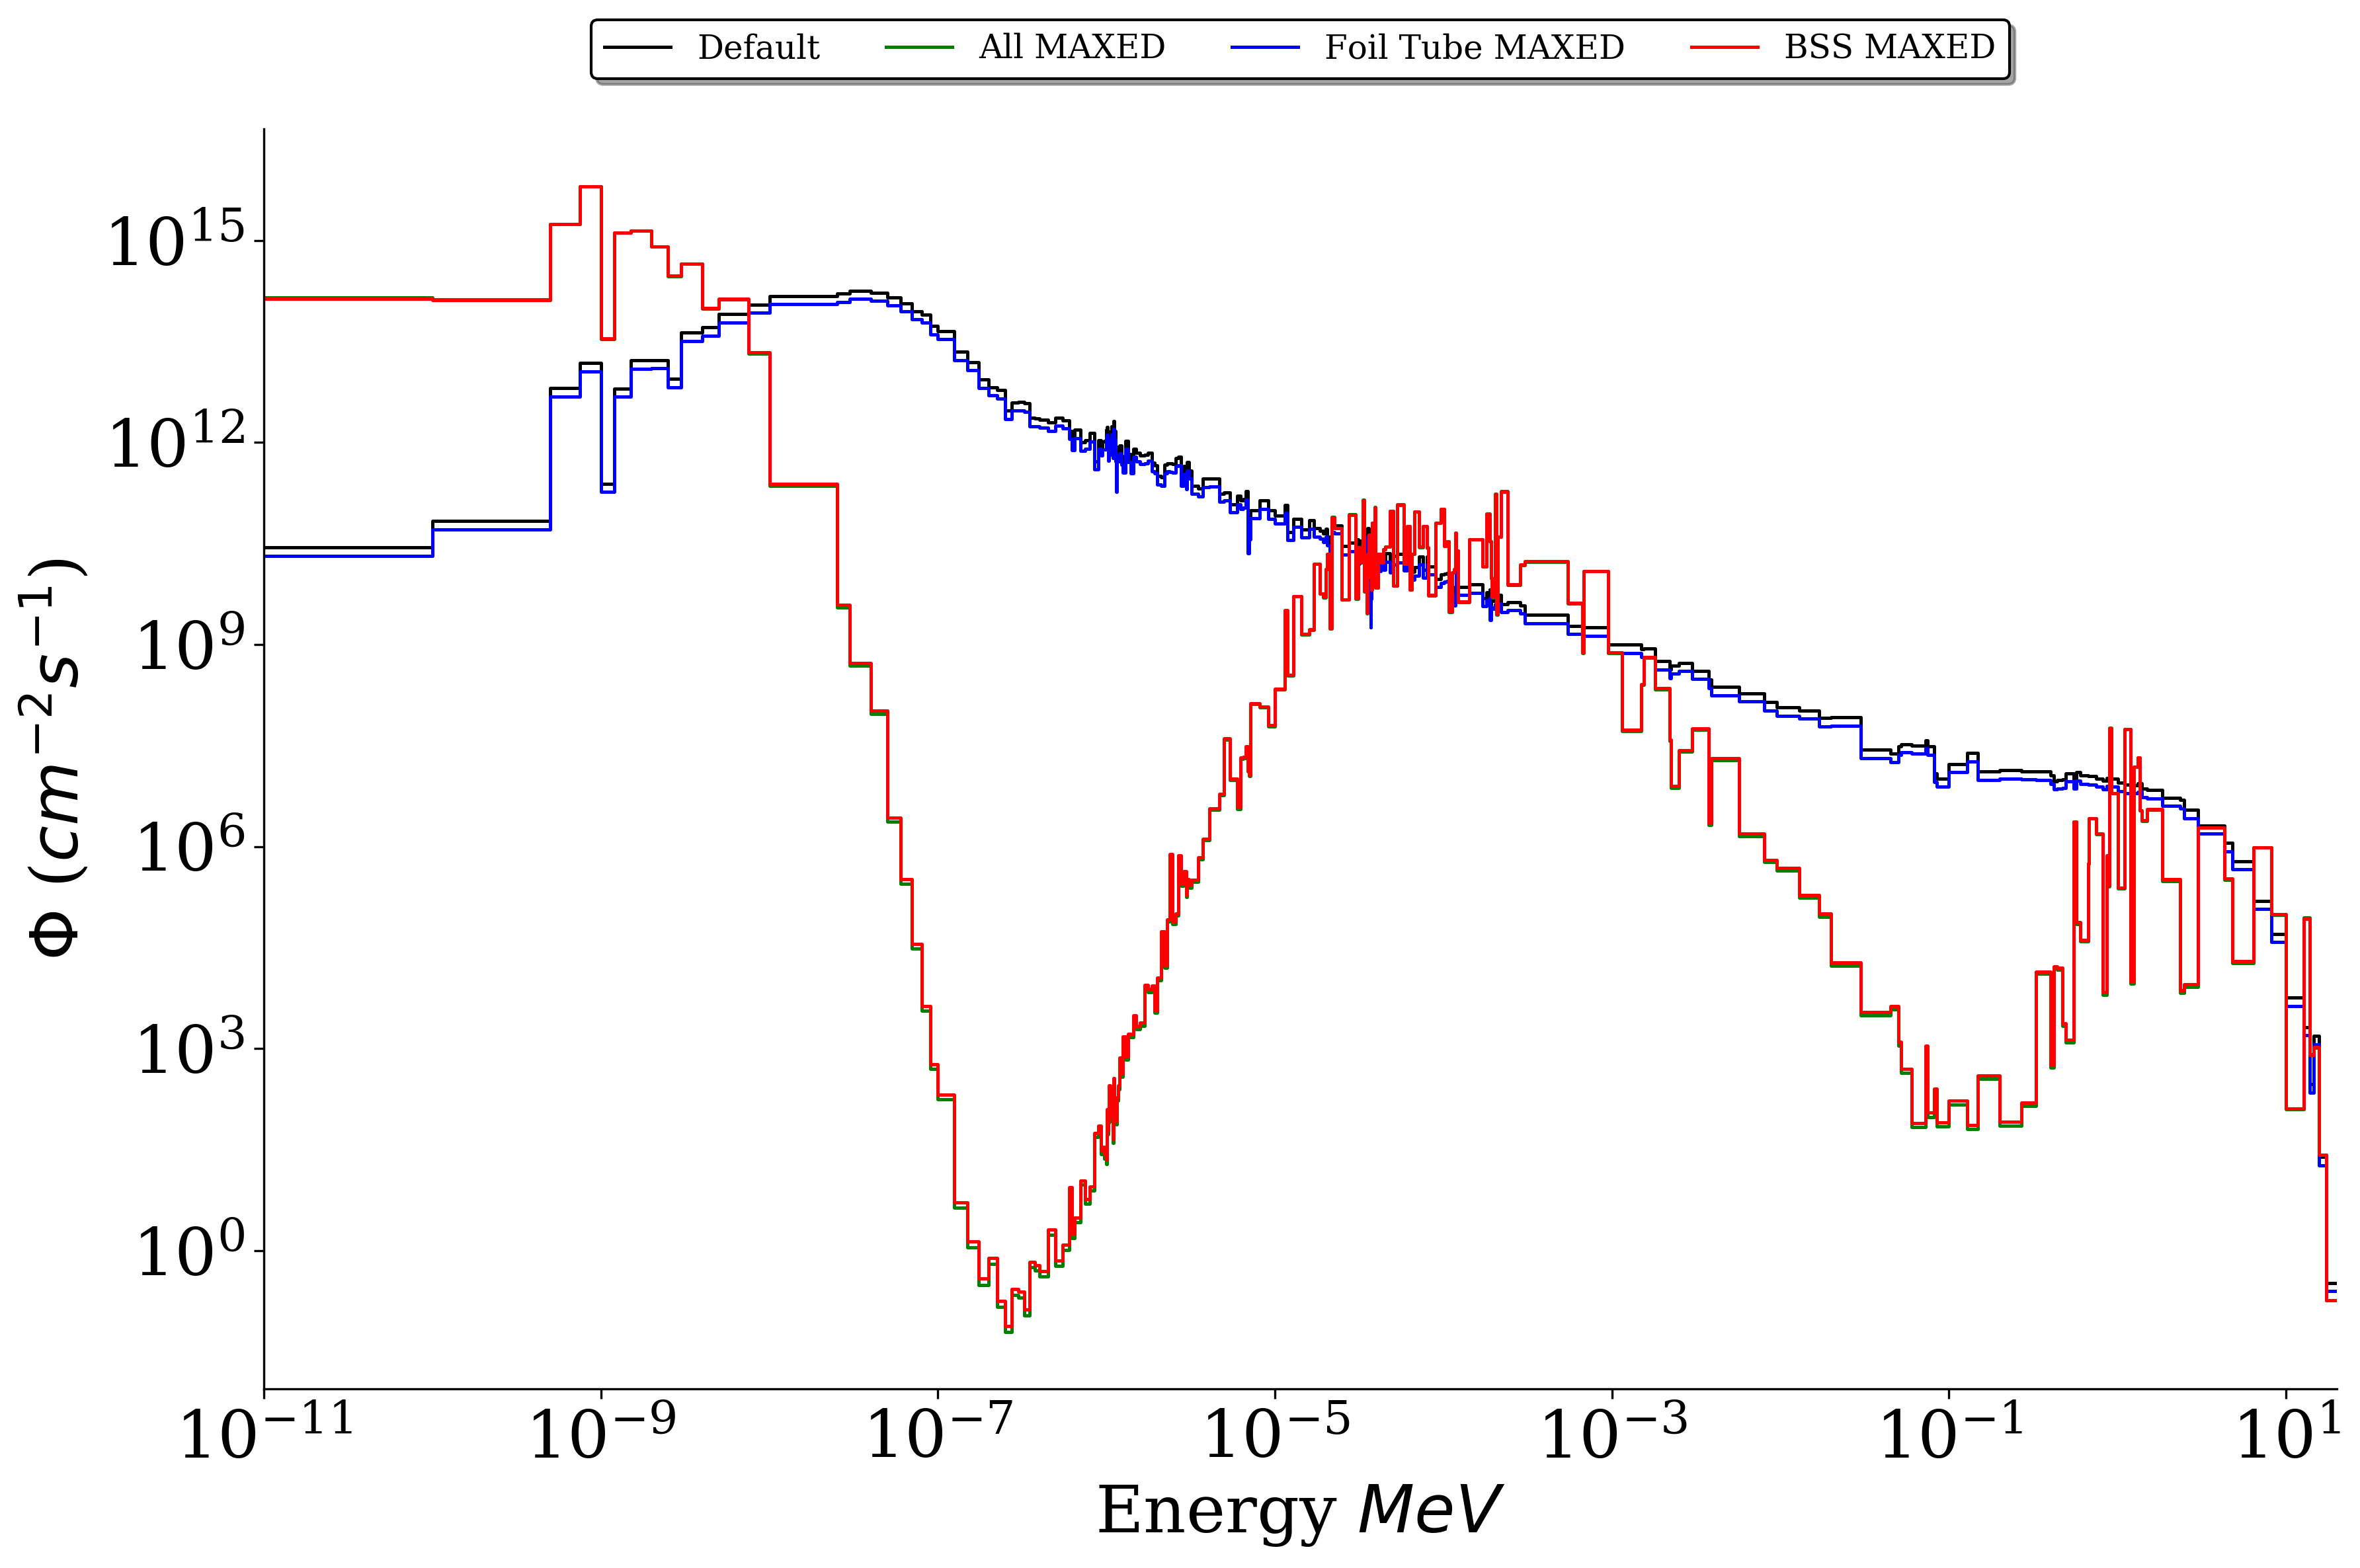
\includegraphics[height=3.8in]{tex/figures/unfolded_mx_sc.png}
\caption[MAXED Unfolded Spectra (Scaled)]{The unfolded NEBP spectra obtained from scaling the default spectrum then unfolding with the MAXED method.}
\label{fig:unfolded_mx_sc}
\end{figure}

% although it was hypothesized that scaling the spectrum would results in a less erratic answer, the results here are very similar in characteristics to the unscaled maxed results
It was hypothesized that scaling the defaults spectrum would remove some of the unphysicalities of the solution spectra; however, the results in \FIG{fig:unfolded_mx_sc} still appear erratic and are very similar in characteristics to the unscaled versions.
% the bss and combined cases are still unphysical, and the ft_au remaines unperturbed
The BSS and combined cases are still rather unphysical, and the foil tube solution remains unperturbed.

\begin{figure}[htb]
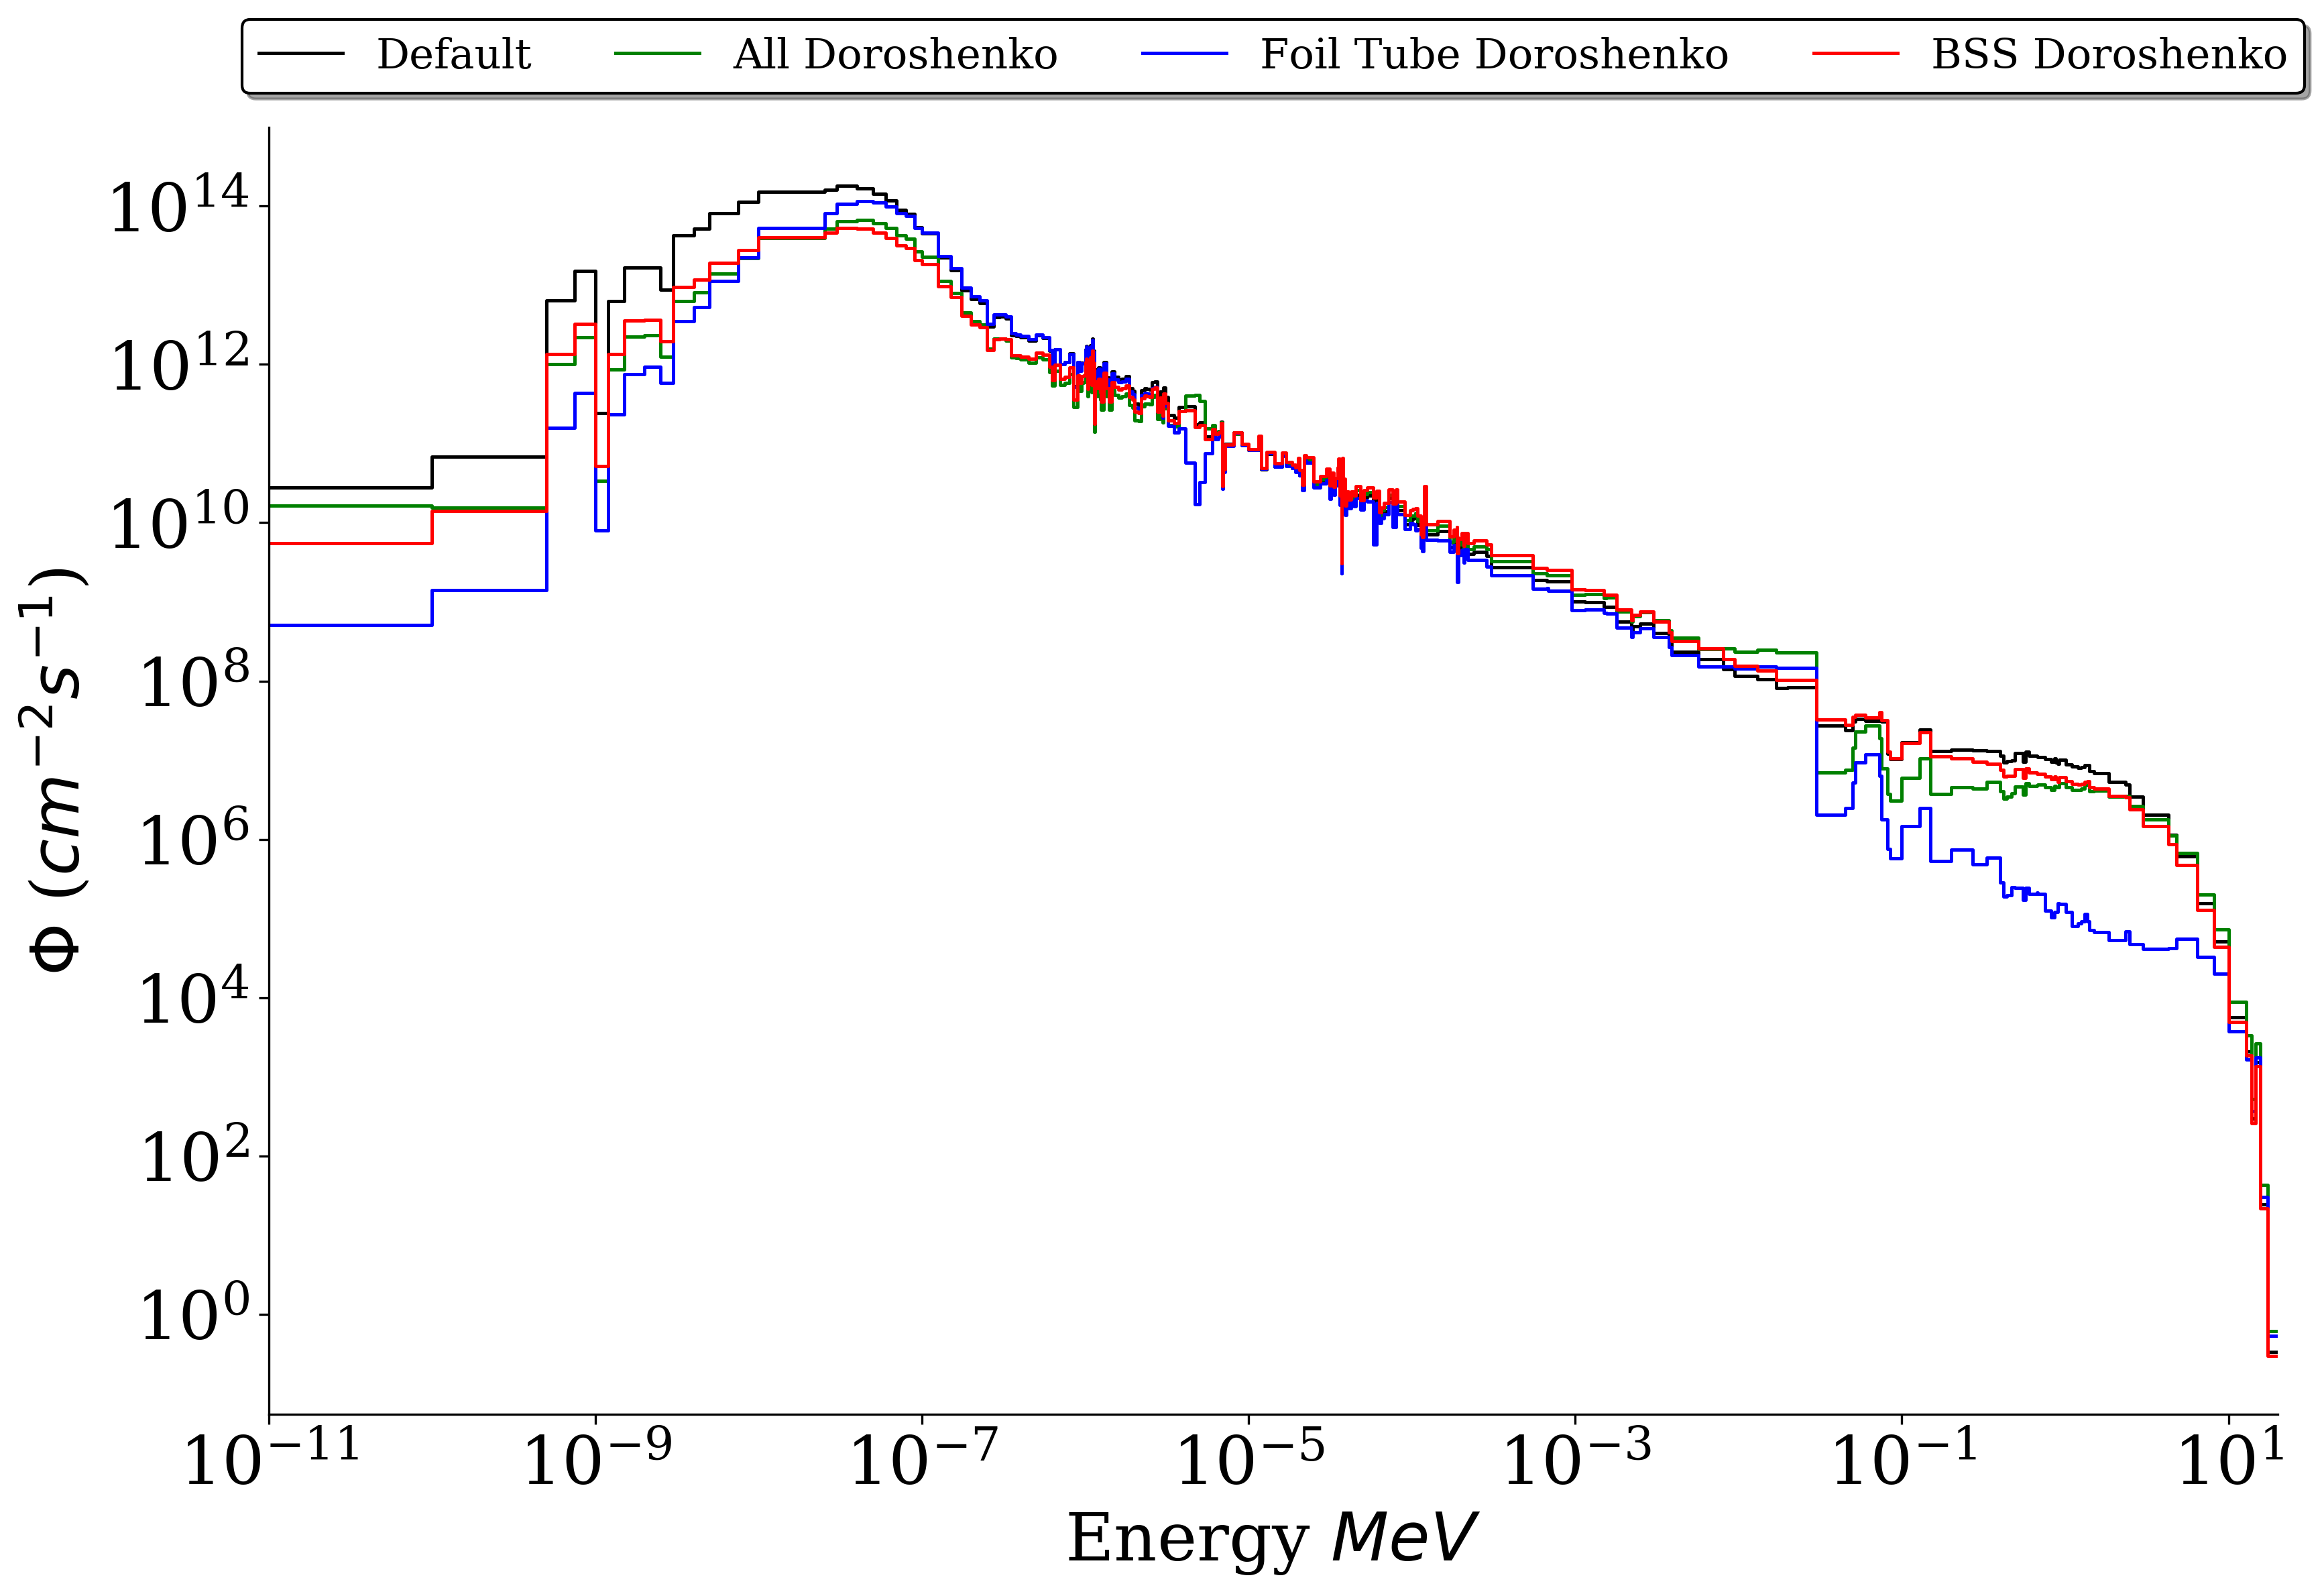
\includegraphics[height=3.8in]{tex/figures/unfolded_do.png}
\caption[Doroshenko Unfolded Spectra]{The unfolded NEBP spectra obtained from unfolding with the Doroshenko method.}
\label{fig:unfolded_do}
\end{figure}

% results in figure are from doroshenko
The results in \FIG{fig:unfolded_do} are from the Doroshenko unfolding.
% unlike maxed, they appear similar to the unfolding with gravel
Unlike MAXED, these results appear stable, like the Gravel data.
% here, though, the differences in the datasets are exemplified
Here, though, the differences between the datasets are more exemplefied.
This is most obvious in the foil tube dataset.
The fast end of the spectrum appears flattened as it tries to fit some of the foil data whose responses lie in that end.
Those responses have high error and likely this feature is due to a bias in the measurement, and not an actual spectral feature.
The other two datasets unfolded into reasonable-appearing spectra, with some slight variation in both the center of the maxwellian distribution, as well as in the flatness of the fast region.



%
\cleardoublepage


\chapter{Conclusions and Future Work}

\section{Conclusions}
%% concise statements about your main findings, related to your aims/objectives/hypothesis.
% it's possible to simulate the beam w/ advantg
First, through the assistance of the VR methods described, it is possible to find the neutron spectrum for a collimated reactor beam port.
% a high resolution flux was obtained via simulation
A high resolution flux spectrum was obtained via Monte Carlo simulation for the KSU TRIGA Mark II's Northeast Beam Port featuring dimensional data in energy, angle, and the radial direction.
% two separate experiments showed data that agreed with the shape of the simulation work and showed similar magnitude differences
Two separate experiments were conducted which collected data that demonstrated decent shape-agreeance with the simulated spectrum and differed in magnitude from the simulated work by similar values.
% the foil tube was novel
Of the two experiments, one involved the creation of a novel type of neutron spectrometer which solved issues like beam alignment and allowed for several different responses to be obtained using only one irradiation and one type of foil (gold).
% successful tuning of spectrum led to a set of solution spectra that is consistent with experimental data
Successful deconvolution using the experimental data led to a set of solution spectra that is consistent with a typical reactor spectrum shape, the original simulated spectrum shape, and the experimental data.
% the shape looks softer than originally hypothesized, resembling an in-core neutron flux
The final shape of the spectrum doesn't match the original hypothesis of being predominately fast, but rather resembles an in-core neutron flux.
% the beam is functionally monodirectional
The final flux is approximately monodirectional.
% a significant majority of the flux is departing from inside the collimator
Also, a significant majority of the flux departing from the beam port lives with the void of the collimator.



\section{Contribution to the field of research}
%% stating/restating the significance of what you have discovered. Can include limitations
% through this analysis we know a lot more about the beam port
Through this analysis, a much more complete picture of the NEBP has been obtained.
% this analysis replaces the old data allowing experimentalists a better understanding of the environment
This replaces the sparse existing data, which allows experimentalists to better understand the environment that their devices will be tested in.
% the set of experiments provides a benchmark for future simulation
The set of experiments conducted provides a set of benchmarks for future simulations of the NEBP.
% this effort led to additions to the ksu reactor model making it more complete
This effort led to several additions to the KSU reactor model, making it more complete.
% steps in this analysis could easily be extended to any reactor beam problem
Many of the steps taken in this analysis could be easily extended to other reactor beam problems, and the success found here allows other analysts the confidence to invest time attempting to simulate their beam in this way.
% the foil tube design is a easy to manufacture device that can be used as a new way to characterize any neutron beam
The foil tube design used here is an easy to manufacture device that can be adapted and used as a new way to characterize a neutron beam.



\section{Future Research}
%% where to go from here (can include where NOT to go, if your research demonstrated that a particular approach or avenue was not useful).
% the other three beam ports should be simulated
Following this work, the other three beam ports at KSU can be characterized in a similar way.
% the framework provided here will extend easily to the other beam ports
The framework provided here will easily extend to those other beam ports and allow the analyses to be done much quicker.
% this includes the experimental methods
This includes the experimental methods utilized.
% work could also be done to study the difference in power/temperature effects as well as the effect control rods may have on the beam port spectrum
Work can also be done to study the difference made on the spectrum by operating the reactor a different powers/temperatures, as well as the effect that different control rod positionings could have on the spectrum.
% the experiments done here should be redone regularly, to consistently benchmark the spectrum
The experiments conducted in this research should be redone regularly to provide a continually evolving understanding of the NEBP spectrum.

% the foil tube alone provides a framework for more research
The foil tube desing alone also provides a framework for more research to be conducted.
% the design could be done with different kinds of foils, and become an optimization problem for spacers, foil types, the inclusion of cadmium
There are many different parameters the device could be optimized for.
This includes the spacer widths and materials, different or multiple foil types, the inclusion of cadmium or some other covering material in the design, and different overall geometric concepts.





% +--------------------------------------------------------------------+
% | References
% +--------------------------------------------------------------------+

% +--------------------------------------------------------------------+
% | Included for Gather Purpose only.  Do NOT uncomment the next line.
%input "tex/refs/references.bib"
% | In order for the WinEDT editor to index references correctly, it
% | has to know where the "references.bib" file resides.  This
% | command will be ignored completely by LaTeX
% |
% | WinEDT can read file path names with either "\" or "/". LaTeX,
% | however,doesn't like "\", so it's easier to store a path name
% | using forward slashes "/".
% +--------------------------------------------------------------------+

\cleardoublepage
\phantomsection

% +--------------------------------------------------------------------+
% | This template uses the BibTeX program to format references.  The
% | lines below create a separate Bibliography section and add
% | an entry for "Bibliography" to the Table of Contents.  The actual
% | data for your references (author, title, journal, date, etc.) are
% | entered in the references.bib file.  See "Citations and Bibliography"
% | for details on to creating citations and formatting references.
% +--------------------------------------------------------------------+

\addcontentsline{toc}{chapter}{Bibliography}
\bibdata{tex/refs/references}
\bibliography{tex/refs/references}

% +--------------------------------------------------------------------+
% | The following commands add the appendices  To add or delete
% | appendices, add or remove the line
% |
% |     \input{appendixX.tex}
% |
% | where "X" is the letter designation of the appendix (A, B, C,
% | etc.) You should have one \input{appendixX.tex} line and a
% | corresponding file appendixX.tex for each appendix.
% |
% |If you do not have any appendices, comment out or delete the three
% |lines below.
% +--------------------------------------------------------------------+

%\appendix
%% +--------------------------------------------------------------------+
% | Appendix A Page (Optional)                                         
% +--------------------------------------------------------------------+

\cleardoublepage

\chapter{Title for This Appendix}

\label{Appendix:Key1}

Enter the content for Appendix A in the appendixA.tex file.  If you
do not have an Appendix A, see comments in the etdrtemplate.tex file
for instructions on how to remove this page.

%% +--------------------------------------------------------------------+
% | Appendix B Page (Optional)                                         
% +--------------------------------------------------------------------+

\cleardoublepage

\chapter{Title for This Appendix}
\label{Appendix:Key2}

Enter the content for Appendix B in the appendixB.tex file. If you
do not have an Appendix B, see comments in the etdrtemplate.tex file
for instructions on how to remove this page.


\end{document}

% +--------------------------------------------------------------------+
% | Template Revisions
% |
% | 9/14/06: Removed typos
% | 3/29/13: Removed hypernat package
% | 4/5/13: Changed to plain bib style
% | 5/17/13: added /cleardoublepage and /phantomsection to
% |          /bibliography to correct TOC page problem
% | 5/17/13: Fixed TOC problem with Dedication, Preface, etc.
% | 12/16/15: Added tocloft package to produce leader dots for all
% |           entries in the table of contents.
% |           Added geometry package to specify 1 inch margins.
% |           Removed unnecessary color specifications.
% |           Changed to \citep for citations.
% | 2/9/2016: Replaced \bibpunct with \setcitestyle.
% |           Changed to unsrtnat style
% |           Added natbib.pdf and Citations and Bibliography.pdf files
% | 8/3/2018: Fixed problem with incorrect page numbers for
% |           Acknowledgements, Dedication, and Preface in TOC.
% |           Removed limit on number of words in Abstract.
% +--------------------------------------------------------------------+
